\documentclass{article}
\usepackage[utf8]{inputenc}
\usepackage{amsmath}
\usepackage{afterpage}
\usepackage{amssymb}
\usepackage{svg}
\usepackage{listings}
\usepackage{physics}
\usepackage{tikz}
\usepackage{pgfplots}
\usepackage{float}
\usepackage{graphicx,wrapfig,lipsum}
\usepackage[makeroom]{cancel}
\usepackage{blindtext}
\usepackage{multicol}
\usepackage[hidelinks]{hyperref}
\usepackage{lipsum}
\usepackage{siunitx}
\usepackage{imakeidx}
\usepackage{cleveref}
\usepackage{subfig}
\usepackage{polynom}
\makeindex[columns=2, title=Indice Alfabetico, intoc]
\pgfplotsset{compat=1.18}
\hypersetup{
    colorlinks=true,
    linkcolor=black,
    urlcolor=magenta
    } 
\AtBeginEnvironment{align}{\setcounter{equation}{0}}
\urlstyle{same}
\usepgfplotslibrary{external,fillbetween}
\usetikzlibrary{arrows.meta}
\restylefloat{table}
\tikzexternalize[prefix=media/cache/]
%Funzioni standard
\pgfmathdeclarefunction{gauss}{2}{\pgfmathparse{1/(#2*sqrt(2*pi))*exp(-((x-#1)^2)/(2*#2^2))}%
}
\begin{document}
    \title{\bf Appunti Comunicazioni Numeriche \par}
\author{Francesco Mignone}
\date{}
\begin{titlepage}

    \maketitle    

    \begin{center}
        Professori:


        Luca Sanguinetti - Marco Moretti

        \vfill
        \begin{figure}[htp]
            \centering
            \includegraphics[width=4cm]{media/uwu.png}
            \caption{uwu}
            \label{fig:uwu}
        \end{figure}
        AA 2022 - 2023
    \end{center}

\end{titlepage}

    \include{1_indice.tex}
    \section{Introduzione}
I seguenti appunti sono presi seguendo le lezioni del corso di Comunicazioni Numeriche 
di Ingegneria Informatica dell'Univertistá di Pisa. Questi appunti non 
vanno a sostituire il materiale e le lezioni dei professori.\\
I testi consigliati sono:

S.Hawking Digital Communication System Wiley


Leon Digital Analog Communication System Pearson


    \section{Richiamo Sui Numeri Complessi}
\subsection{Struttura di un numero complesso}

    \subsubsection{Forma Cartesiana}
            \begin{center}
                \[
                  z \in \mathbb{C} : z = a + jb
                \]
                Parte reale: $a=Re\{z\}$


                \vspace{0.1cm}
                Parte Immaginaria: $b=Img\{z\}$

                \vspace{0.1cm}
                {\em j} o {\em i} é la $\sqrt{-1}$  
            \end{center}
            
    \subsubsection{Forma Polare}
        \begin{center}
            \[
                z \in \mathbb{C} : z = \rho \ e^{j\theta}
            \]
            Modulo: $\rho = |z|$


            \vspace{0.1cm}
            Fase: $\theta = \arg(z)$
        \end{center}    
        grafico forma polare-cartesiana
        
    \subsubsection{Complesso Coniugato}
        \begin{itemize}
            \item {Forma Cartesiana   
                    \[
                        z^* = a - jb
                    \]
            }
            \item {Forma Polare
                    \[
                        z^* = \rho \ e^{-j\theta}
                    \]
            }           
        \end{itemize}


\subsection{Relazione Tra Forma Polare e Cartesiana}
    \begin{itemize}
        \item {Parte Reale e parte Immaginaria
            \[
                a = \rho \cos(\theta)  \ \ b = \rho \sin(\theta)   
            \]
        }
        \item {Modulo
            \[
                \rho = |z| = \sqrt{a^2+b^2}
            \]
        }
        \item {Fase
            \[
                 a \\> 0 \Rightarrow \theta = \arg(z) = \arctan\left(\frac{b}{a}\right)
            \]
            \[
                a \\< 0 \Rightarrow \theta = \arg(z) =\pi + \arctan\left(\frac{b}{a}\right) 
            \]

        }
    \end{itemize}


\subsection{Operazioni}
    Dati: $z_1 = a_1 + jb_1 = \rho_1 \ e^{j\theta_1},\hspace{0.1cm} z_2 = a_2 + jb_2 = \rho_2 \ e^{j\theta_2} $
    \begin{itemize}
        \item {Somma
            \[
                z = z_1 + z_2 = (a_1 + a_2) + j(b_1 + b_2)
            \]
        }
        \item {Sottrazione
            \[
                z = z_1 - z_2 = (a_1 - a_2) + j(b_1 - b_2)
            \]
        }
        \item {Moltiplicazione
            \[
                z = z_1 z_2 = \rho_1\rho_2 \ e^{j(\theta_1+\theta_2)}
            \]
        }
        \item {Divisione
            \[
                z = \frac{z_1}{z_2} = \frac{\rho_1}{\rho_2} \ e^{j(\theta_1-\theta_2)}
            \]
        }
        \item {Modulo
            \[
                |z| = \sqrt{zz^*} = \sqrt{a^2+b^2}  
            \]
            \[
                |z|^2 = zz^* = a^2+b^2  
            \]
        }
    \end{itemize}

    \subsection{Funzioni Complesse a Variabile Reale}
        \[
           z \in \mathbb{C} \hspace{0.2cm} t \in \mathbb{R} \rightarrow z_{(t)} = a_{(t)} + jb_{(t)} = \rho_{(t)} e^{j\theta_{(t)}}
        \]
        \begin{itemize}
            \item {Integrale
            \[
                \int_{a}^{b} z_{(t)} \ dt = \int_{a}^{b} a_{(t)} + jb_{(t)} \ dt =\int_{a}^{b} a_{(t)} \ dt+\int_{a}^{b} jb_{(t)} \ dt  
            \]

            }
            \item {Derivata
            \[
                \frac{d}{dt} z_{(t)}= \frac{d}{dt} a_{(t)} + jb_{(t)} =\frac{d}{dt} a_{(t)} +\frac{d}{dt} jb_{(t)}   
            \]

            }
        \end{itemize}

    \section{Introduzione Ai Segnali}
Segnale
    \subsection{Tipologie di Segnali}
    \section{Segnali Analogici}
    \subsection{Grandezze dei segnali Analogici}
    
        \subsubsection{Potenza istantanea}
            \[
                P_{x} \triangleq |x_{(t)}|^2   
            \]
        \subsubsection{Energia}
            \[
                E_{x} \triangleq \int_{-\infty}^{\infty} P_{x}(t) \,dt = \int_{-\infty}^{\infty} |x_{(t)}|^2 \,dt    
            \]
        \subsubsection{Potenza Media}
            Definiamo il \index{Segnale Troncato}{\bf Segnale Troncato}:
                \[
                    x_{(t)} = X_{(t)} \triangleq 
                    \begin{cases}
                        x_{(t)} \hspace{1cm} -\frac{T}{2} \leq t \leq \frac{T}{2} \\
                        0 \hspace{2cm}altrove
                    \end{cases}
                    \]  
                    \begin{center}
                        \em T = Periodo di osservazione
                    \end{center}
                \begin{figure}[h]
                    \centering
                    \includegraphics[width=4cm]{media/uwu.png}
                    \caption{Segnale troncato}
                    \label{fig:troncato}
                \end{figure}
            

            % NON CAPISCO COSA É POTENZA MEDIA E COSA SIA POTENZA ISTANTANEA CHE CAVOLO DI RELAZIONE
            % USO PER PASSARE DA PxT A Px  
            La potenza media é:
            \[
                P_{x_{T}} \triangleq E_{x_{T}}   
            \]
            dalla quale possiamo ricavare la potenza istantanea se $T \rightarrow \infty \Rightarrow P_{x_{T}} = P_{x}$:
            \[
                P_{x} \triangleq \lim_{T\rightarrow\infty} \frac{E_{x_{T}}}{T} =\lim_{T\rightarrow\infty} \frac{1}{T} \int_{-\frac{T}{2}}^{\frac{T}{2}}  |x_{(t)}|^2 \,dt    
            \]  
        \subsubsection{Valore Efficace}
        
        \subsubsection{Valore Medio}

    \subsection{Analisi energetiche su segnali comuni}
        \subsubsection{Costante}

        \subsubsection{Sinusoide}
        
        \subsubsection{Gradino}
        
        \subsubsection{Rettangolo}
        
        \subsubsection{Esponenziale unilatera}
        
        \subsubsection{Esponenziale bilatera}
        
        \subsubsection{segno $\mathbf{sgn(x_{(t)})}$}
    \section{Trasformata Serie Di Fourier}
    \subsection{Segnale Periodico}
        Si definisce segnale periodico un segnale tale che:
        \[
            x_{(t)} = x_{(t-kT_0)}    
        \]
        \[
            T_0=Periodo\ \ \ f_0\triangleq \frac{1}{T_0} =Frequenza
        \]
    \subsection{Trasformata Serie Di Fourier}
        Ogni segnale periodico di periodo $T_0$ che soddifa le condizioni di Dirichlet e la sua $E_x < \infty (C.S.)$ puó essere scritto come la somma di 
        infinite sinusoidi di frequenze multiple di $f_0 = \frac{1}{T_0}$
        \begin{itemize}
            \item{Equazione di Sintesi - Antitrasformata(ATSF)\label{ATSF}
                \[
                    x_{(t)} = \sum_{k = -\infty}^{\infty} X_{k} e^{j2\pi kf_0t} \hspace{1cm} X_{k}\in \mathbb{C},\ f_0 = \frac{1}{T_0} 
                \]
                Se lo sviluppassimo sarebbe composto da:
                \[
                   x_{(t)} =\ldots  + X_{-1} e^{j2\pi (-1)f_0t} + X_{0} + X_{1} e^{j2\pi (1) f_0t} + \ldots 
                \]
                $X_0$ corrisponde al Valore medio \ref{Valore medio} del segnale, inoltre le componenti $X_k$ prendono il nome di armoniche alla frequenza $f$ corrispondente
            }
            \item{Equazione di Analisi - Trasformata(TSF)\label{TSF}
                \[
                    X_k =\frac{1}{T_0}\int_{-\frac{T_0}{2}}^{\frac{T_0}{2}} x_{(t)} e^{-j2\pi kf_0t} dt
                \]
            } 
        \end{itemize}
        La TSF gode della biunivocitá: $\forall x_{(t)} \exists! X_k$:
        \begin{align}
            x_{(t)} & \overunderset{TSF}{ATSF}{\rightleftharpoons} X_k  \nonumber\\
            Segnale\ Analogico\ Periodico &\overunderset{TSF}{ATSF}{\rightleftharpoons} Sequenza\ Complessa \nonumber
        \end{align}
        \subsubsection{Rappresentazione di $X_k$}
            Essendo $X_k$ un numero complesso puó essere rappresentato in forma polare: 
            \[
                X_k = |X_k|e^{\angle X_k}  
            \]
            Si possono rappresentare il modulo (Ampiezza) e la fase tramite grafici che prendono il nome di spettri:
            \begin{figure}[H]
                \centering
                \subfloat[Spettro di Ampiezza]{
                    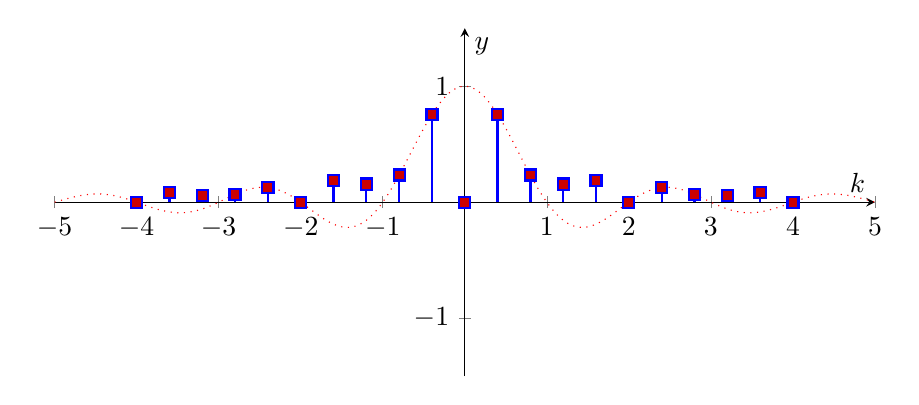
\begin{tikzpicture}
                        \begin{axis}[
                            domain=-5:5,
                            samples=200,
                            axis lines=middle,
                            xlabel=$k$,
                            ylabel=$y$,
                            ymin=-1.5,
                            ymax=1.5,
                            xtick={-5,-4,-3,-2,-1,0,1,2,3,4,5},
                            xticklabels={$-5$,$-4$,$-3$,$-2$,$-1$,$0$,$1$,$2$,$3$,$4$,$5$},
                            ytick={-1, 1},
                            yticklabels={$-1$, $1$},
                            width=12cm,
                            height=6cm
                        ]
                        \addplot [red,dotted, samples = 300] {sin(deg(x*pi))/(x*pi)};
                        \addplot+ [blue, thick, ycomb, samples at={-4,-3.6,-3.2,-2.8,-2.4,-2,-1.6,-1.2,-0.8,-0.4,0,0.4,0.8,1.2,1.6,2,2.4,2.8,3.2,3.6,4}] {abs(sin(deg(x*pi))/(x*pi))};
                        \end{axis}
                    \end{tikzpicture}
                }
                \hfill
                \subfloat[Spettro di Fase]{
                    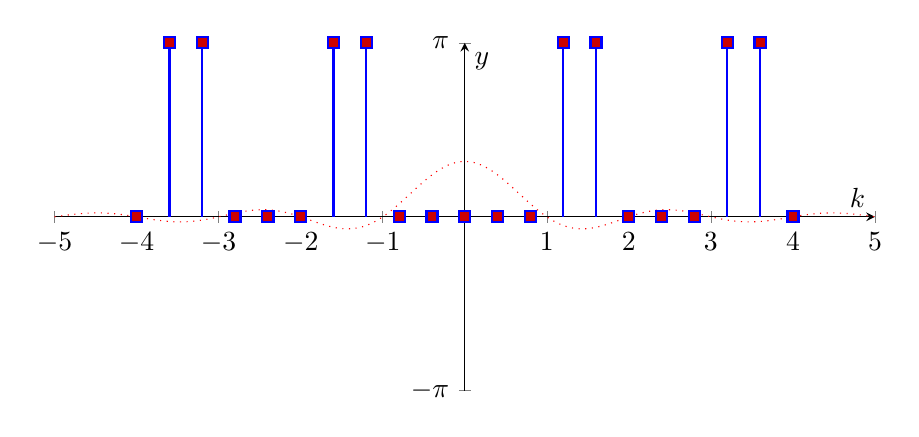
\begin{tikzpicture}
                        \begin{axis}[
                            domain=-5:5,
                            samples=200,
                            axis lines=middle,
                            xlabel=$k$,
                            ylabel=$y$,
                            ymin=-pi,
                            ymax=pi,
                            xtick={-5,-4,-3,-2,-1,0,1,2,3,4,5},
                            xticklabels={$-5$,$-4$,$-3$,$-2$,$-1$,$0$,$1$,$2$,$3$,$4$,$5$},
                            ytick={-pi, pi},
                            yticklabels={$-\pi$, $\pi$},
                            width=12cm,
                            height=6cm
                        ]
                        \addplot [red,dotted, samples = 300] {sin(deg(x*pi))/(x*pi)};
                        \addplot+ [blue, thick, ycomb, samples at={-4,-3.6,-3.2,-2.8,-2.4,-2,-1.6,-1.2,-0.8,-0.4,0,0.4,0.8,1.2,1.6,2,2.4,2.8,3.2,3.6,4}] {rad(atan2(0,sin(deg(x*pi))/(x*pi)))};
                        \end{axis}
                    \end{tikzpicture}
                }
                \caption{Spettro di un treno di rect}
            \end{figure}
            lo spettro di Ampiezza gode della \textbf{simmetria pari} rispetto alle ascisse quindi é \textbf{sempre positivo}, mentre lo spettro di fase della \textbf{simmetria dispari}.
        \subsection{Propietá della TSF}
            \subsection{Linearitá}
            \subsection{Simmetria Hermitiana}
        
        \subsection{Calcolo dei coefficienti $X_k$ per segnali noti}
            \subsubsection{$A\cos(2\pi f_0 t)$}
                $x_{(t)}=A\cos(2\pi f_0 t), \hspace{0.3cm} A>0$
                \begin{align}
                    ATSF[x_{(t)}] & = ATSF[A\cos(2\pi f_0 t)] \nonumber \\
                        & = ATSF[\frac{A}{2} (e^{j2\pi kf_0t} + e^{-j2\pi kf_0t})] \nonumber 
                \end{align}
                Utilizzando la composizione dei coefficienti $X_k$:
                \begin{align}
                    x_{(t)} & =\ldots  + X_{-1} e^{j2\pi (-1)f_0t} + X_{0} + X_{1} e^{-j2\pi (1) f_0t} + \ldots \nonumber\\
                    Abbiamo:& \nonumber 
                \end{align}
                        \[X_{-1} = \frac{A}{2}\hspace{.3cm} X_{0} = 0\hspace{.3cm} X_{1} = \frac{A}{2}\] 
                Possiamo tracciare lo spettro del segnale:
                \begin{figure}[H]
                    \centering
                    \subfloat[Spettro di Ampiezza]{
                    \begin{tikzpicture}
                        \begin{axis}[
                            domain=-4:4,
                            samples=200,
                            axis lines=middle,
                            xlabel=$t$,
                            ylabel=$y$,
                            ymin=-1.5,
                            ymax=1.5,
                            xtick={-5,-4,-3,-2,-1,0,1,2,3,4,5},
                            xticklabels={$-5$,$-4$,$-3$,$-2$,$-1$,$0$,$1$,$2$,$3$,$4$,$5$},
                            ytick={1},
                            yticklabels={$\frac{A}{2}$},
                            width=6.5cm,
                            height=5cm
                            ]
                            \addplot [const plot,black,dotted] coordinates{(-4,1)(4,1)};
                            \addplot+ [blue, thick, ycomb, samples at = {-1,1}] {1};
                            \end{axis}
                        \end{tikzpicture}
                    }
                    \hfill
                    \subfloat[Spettro di Fase]{
                        \begin{tikzpicture}
                            \begin{axis}[
                                domain=-4:4,
                                samples=200,
                                axis lines=middle,
                                xlabel=$t$,
                                ylabel=$y$,
                                ymin=-pi,
                                ymax=pi,
                                xtick={-5,-4,-3,-2,-1,0,1,2,3,4,5},
                                xticklabels={$-5$,$-4$,$-3$,$-2$,$-1$,$0$,$1$,$2$,$3$,$4$,$5$},
                                ytick={-pi, pi},
                                yticklabels={$-\pi$, $\pi$},
                                width=6.5cm,
                                height=5cm
                            ]
                            \addplot+ [blue, thick, ycomb, samples at = {-4,-3,-2,-1,0,1,2,3,4}] {0};
                            \end{axis}
                        \end{tikzpicture}
                    }
                    \caption{Spettro TSF del coseno $A>0$}
                \end{figure}
            \subsubsection{$A\sin(2\pi f_0 t)$}
                $x_{(t)}=A\sin(2\pi f_0 t), \hspace{0.3cm} A>0$
                \begin{align}
                    ATSF[x_{(t)}] & = ATSF[A\sin(2\pi f_0 t)] \nonumber \\
                        & = ATSF[\frac{A}{2} (e^{j2\pi kf_0t} - e^{-j2\pi kf_0t})] \nonumber 
                \end{align}
                Utilizzando la composizione dei coefficienti $X_k$:
                \begin{align}
                    x_{(t)} & =\ldots  + X_{-1} e^{j2\pi (-1)f_0t} - X_{0} + X_{1} e^{-j2\pi (1) f_0t} + \ldots \nonumber\\
                    Abbiamo:& \nonumber 
                \end{align}
                        \[X_{-1} = -\frac{A}{2j}\hspace{.3cm} X_{0} = 0\hspace{.3cm} X_{1} = \frac{A}{2j}\] 
                \[
                    |X_k|= 
                    \begin{cases}
                            |\frac{A}{2j}| = \frac{A}{2} \hspace{0.5cm} & k= 1\\
                            |-\frac{A}{2j}| = \frac{A}{2} \hspace{0.5cm} & k= -1\\
                            0 \hspace{0.5cm} & altrove  \\
                    \end{cases}
                    \hspace{0.5cm}
                    \angle X_k= 
                    \begin{cases}
                        \angle \frac{A}{2j} = -\frac{\pi}{2} \hspace{0.5cm} & k= 1\\
                        \angle |-\frac{A}{2j}| = \frac{\pi}{2} \hspace{0.5cm} & k= -1\\
                        0 \hspace{0.5cm} & altrove  \\
                    \end{cases}
                    \]
                Possiamo tracciare lo spettro del segnale:
                \begin{figure}[H]
                    \centering
                    \subfloat[Spettro di Ampiezza]{
                        \begin{tikzpicture}
                            \begin{axis}[
                                domain=-4:4,
                                samples=200,
                                axis lines=middle,
                                xlabel=$t$,
                                ylabel=$y$,
                                ymin=-1.5,
                                ymax=1.5,
                                xtick={-5,-4,-3,-2,-1,0,1,2,3,4,5},
                                xticklabels={$-5$,$-4$,$-3$,$-2$,$-1$,$0$,$1$,$2$,$3$,$4$,$5$},
                                ytick={1},
                                yticklabels={$\frac{A}{2}$},
                                width=6.5cm,
                                height=5cm
                                ]
                                \addplot [const plot,black,dotted] coordinates{(-4,1)(4,1)};
                                \addplot+ [blue, thick,mark = triangle*, ycomb, samples at = {-1,1}] {1};
                                \end{axis}
                            \end{tikzpicture}
                        }
                    \hfill
                    \subfloat[Spettro di Fase]{
                            \begin{tikzpicture}
                                \begin{axis}[
                                    domain=-4:4,
                                    samples=200,
                                    axis lines=middle,
                                    xlabel=$t$,
                                    ylabel=$y$,
                                    ymin=-pi,
                                    ymax=pi,
                                    xtick={-5,-4,-3,-2,-1,0,1,2,3,4,5},
                                    xticklabels={$-5$,$-4$,$-3$,$-2$,$-1$,$0$,$1$,$2$,$3$,$4$,$5$},
                                    ytick={-pi,-1/2*pi,1/2*pi, pi},
                                    yticklabels={$-\pi$,$-\frac{\pi}{2}$,$\frac{\pi}{2}$ $\pi$},
                                    yticklabel style = {xshift=3pt}, 
                                    width=6.5cm,
                                    height=5cm
                                ]
                                \addplot+ [blue, thick,mark = square*,const plot] coordinates{(-1,1/2*pi)(-1,0)};
                                \addplot+ [blue, thick,mark = square*,const plot] coordinates{(1,-1/2*pi)(1,0)};

                                \addplot [black, dotted,const plot] coordinates{(-3,-1/2*pi)(3,-1/2*pi)};
                                \addplot [black, dotted,const plot] coordinates{(-3,1/2*pi)(3,1/2*pi)};
                                \end{axis}
                            \end{tikzpicture}
                        }
                    \caption{Spettro TSF del seno $A>0$}
                \end{figure}
            \subsubsection{Treno di rect}
                $x_R=A\hspace{0.1cm}rect\left(\frac{t}{T}\right)\rightarrow$ Segnale periodico $\rightarrow x_{(t)} = \sum_{-\infty}^{\infty} x_R (t-nT_0)$\\
                $T_0 = periodo$, $T = durata \rightarrow T < T_0$, se cosi non fosse avremmo una costante
                \begin{figure}[H]
                    \centering
                    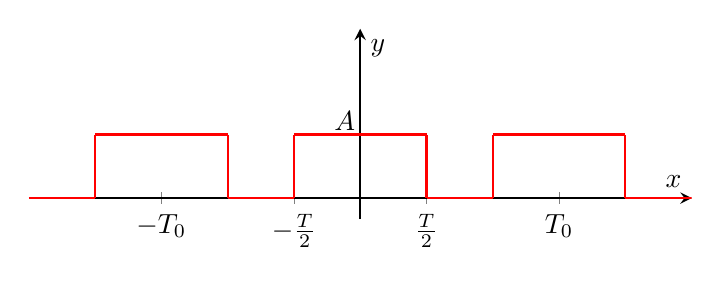
\begin{tikzpicture}
                        \begin{axis}[
                            xlabel=$x$,
                            ylabel=$y$,
                            xmin=-5,
                            xmax=5,
                            ymin=-0.5,
                            ymax=4,
                            ytick = {1.5},
                            xtick={-3,-1, 0, 1,3},
                            xticklabels={$-T_0$,$-\frac{T}{2}$, $0$, $\frac{T}{2}$,$T_0$},
                            yticklabels = {$A$},
                            yticklabel style = {yshift=5pt,xshift=4pt}, 
                            axis lines=middle,
                            thick,
                            domain=-5:5,
                            samples=100,
                            width=10cm,
                            height=4cm
                        ]
                        \addplot [const plot,red, thick] coordinates{(-1,1.5)(1,1.5)};
                        \addplot [const plot,red, thick] coordinates{(-1,0)(-1,1.5)};
                        \addplot [const plot,red, thick] coordinates{(1,0)(1,1.5)};
                        
                        \addplot [const plot,red, thick] coordinates{(-2,1.5)(-4,1.5)};
                        \addplot [const plot,red, thick] coordinates{(-2,0)(-2,1.5)};
                        \addplot [const plot,red, thick] coordinates{(-4,0)(-4,1.5)};
                        
                        \addplot [const plot,red, thick] coordinates{(2,1.5)(4,1.5)};
                        \addplot [const plot,red, thick] coordinates{(2,0)(2,1.5)};
                        \addplot [const plot,red, thick] coordinates{(4,0)(4,1.5)};
                        
                        \addplot [const plot,red, thick] coordinates{(2,0)(1,0)};
                        \addplot [const plot,red, thick] coordinates{(-2,0)(-1,0)};
                        \addplot [const plot,red, thick] coordinates{(-4,0)(-5,0)};
                        \addplot [const plot,red, thick] coordinates{(4,0)(5,0)};
                    
                        \end{axis}
                    \end{tikzpicture}
                    \caption{Treno di $A\hspace{0.1cm}rect\left(\frac{t}{T}\right)$}
                    \label{fig:treno di rect}
                \end{figure}                
                $\rightarrow$ Si nota come cambiare il periodi delle funzioni possiamo renderle da aperiodiche a periodiche e viceversa
                \begin{align}
                    ATSF[x_{(t)}] & = ATSF[\sum_{-\infty}^{\infty} x_R (t-nT_0)] \nonumber \\
                        & = \frac{1}{T_0} \int_{-\frac{T_0}{2}}^{\frac{T_0}{2}} x_{(t)} e^{-j2\pi kf_0t} dt = \frac{1}{T_0} \int_{-\frac{T}{2}}^{\frac{T}{2}} x_{(t)} e^{-j2\pi kf_0t} dt \nonumber \\
                        & = \frac{A}{T_0} \int_{-\frac{T}{2}}^{\frac{T}{2}} e^{-j2\pi kf_0t} dt = \eval{\frac{A}{T_0} \frac{1}{j2\pi kf_0} e^{-j2\pi kf_0t}}_{-\frac{T}{2}}^{\frac{T}{2}} \nonumber \\
                        & = \frac{A}{T_0} \frac{e^{-j\pi kf_0T} - e^{j\pi kf_0T}}{j2\pi kf_0} = \frac{A}{T_0} \frac{e^{j\pi kf_0T}-e^{-j\pi kf_0T}}{-j2\pi kf_0} \nonumber \\
                        & = \frac{A\color{purple}{T}}{T_0} \frac{e^{j\pi kf_0T}-e^{-j\pi kf_0T}}{-j2\pi kf_0\color{purple}{T}} = Af_0T sinc(kf_0T) \nonumber 
                \end{align}
                Tracciamo lo spettro per $f_0T<1$:
                \begin{figure}[H]
                    \centering
                    \subfloat[Spettro di Ampiezza]{
                        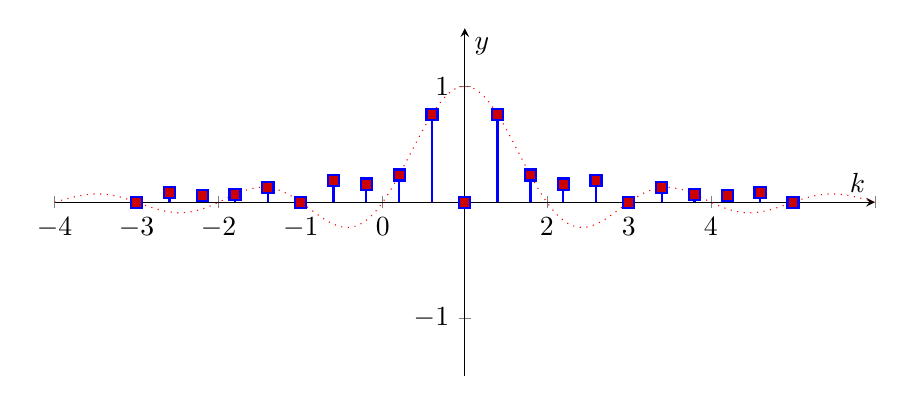
\begin{tikzpicture}
                            \begin{axis}[
                                domain=-5:5,
                                samples=200,
                                axis lines=middle,
                                xlabel=$k$,
                                ylabel=$y$,
                                ymin=-1.5,
                                ymax=1.5,
                                xtick={-5,-4,-3,-2,-1,0,1,2,3,4,5},
                                xticklabels={$-4$,$-3$,$-2$,$-1$,$0$,$1$,$2$,$3$,$4$},
                                ytick={-1, 1},
                                yticklabels={$-1$, $1$},
                                width=12cm,
                                height=6cm
                            ]
                            \addplot [red,dotted, samples = 300] {sin(deg(x*pi))/(x*pi)};
                            \addplot+ [blue, thick, ycomb, samples at={-4,-3.6,-3.2,-2.8,-2.4,-2,-1.6,-1.2,-0.8,-0.4,0,0.4,0.8,1.2,1.6,2,2.4,2.8,3.2,3.6,4}] {abs(sin(deg(x*pi))/(x*pi))};
                            \end{axis}
                        \end{tikzpicture}
                    }
                    \hfill
                    \subfloat[Spettro di Fase]{
                        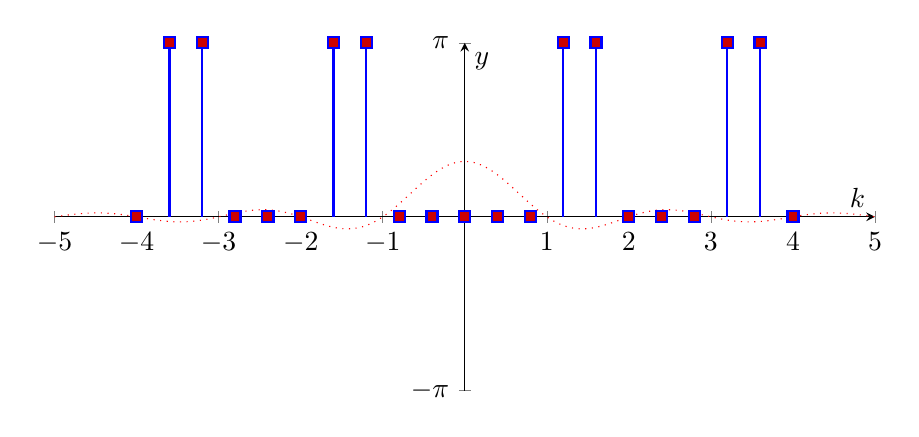
\begin{tikzpicture}
                            \begin{axis}[
                                domain=-5:5,
                                samples=200,
                                axis lines=middle,
                                xlabel=$k$,
                                ylabel=$y$,
                                ymin=-pi,
                                ymax=pi,
                                xtick={-5,-4,-3,-2,-1,0,1,2,3,4,5},
                                xticklabels={$-5$,$-4$,$-3$,$-2$,$-1$,$0$,$1$,$2$,$3$,$4$,$5$},
                                ytick={-pi, pi},
                                yticklabels={$-\pi$, $\pi$},
                                width=12cm,
                                height=6cm
                            ]
                            \addplot [red,dotted, samples = 300] {sin(deg(x*pi))/(x*pi)};
                            \addplot+ [blue, thick, ycomb, samples at={-4,-3.6,-3.2,-2.8,-2.4,-2,-1.6,-1.2,-0.8,-0.4,0,0.4,0.8,1.2,1.6,2,2.4,2.8,3.2,3.6,4}] {rad(atan2(0,sin(deg(x*pi))/(x*pi)))};
                            \end{axis}
                        \end{tikzpicture}
                    }
                    \caption{Spettro TSF del treno di rect con $f_0T<1$}
                \end{figure}
                Si possono anche unire i due spettri per ottenere: 
                \begin{figure}[H]
                    \centering
                    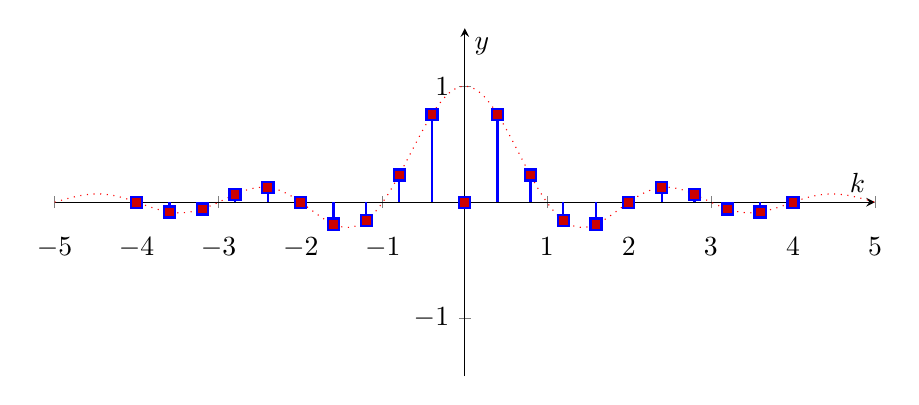
\begin{tikzpicture}
                        \begin{axis}[
                            domain=-5:5,
                            samples=200,
                            axis lines=middle,
                            xlabel=$k$,
                            ylabel=$y$,
                            ymin=-1.5,
                            ymax=1.5,
                            xtick={-5,-4,-3,-2,-1,0,1,2,3,4,5},
                            xticklabels={$-5$,$-4$,$-3$,$-2$,$-1$,$0$,$1$,$2$,$3$,$4$,$5$},
                            ytick={-1, 1},
                            yticklabels={$-1$, $1$},
                            xticklabel style = {yshift=-7pt}, 
                            width=12cm,
                            height=6cm
                        ]
                        \addplot [red,dotted, samples = 300] {sin(deg(x*pi))/(x*pi)};
                        \addplot+ [blue, thick, ycomb, samples at={-4,-3.6,-3.2,-2.8,-2.4,-2,-1.6,-1.2,-0.8,-0.4,0,0.4,0.8,1.2,1.6,2,2.4,2.8,3.2,3.6,4}] {sin(deg(x*pi))/(x*pi)};
                        \end{axis}
                    \end{tikzpicture}
                    \caption{Spettro treno di $A\hspace{0.1cm}rect\left(\frac{t}{T}\right)$}
                    \label{fig:Spettro treno di rect}
                \end{figure}  
            Ora appizza matlab e fa esempi di un segnale e uno di ricostruzione dello stesso(script di matlab presenti nel teams):
            \begin{itemize}
                \item Se un segnale varia molto rapidamente nel tempo ha componenti frequenziali piú alte $\rightarrow$ copre piú spettro(espansione spettrale) $T_0 \Downarrow$
                \item Se un segnale varia molto lentamente copre le basse fraquenze $ T_0 \Uparrow$
            \end{itemize}
            Se non ho abbastanza passi K non posso campionare le alte frequenze e quindi non faccio ne un analisi completa del segnale né riesco a ricostruire perfettamente il segnale  
            Inoltre in $0$ dello spettro ho il Valor medio \ref{Valore medio} del segnale.
    \section{Trasformata Continua Di Fourier}
    \section{Sistemi Monodimensionali}
    Definiamo il Sistema Monodimensionale: 
    \begin{figure}[H]
        \centering 
        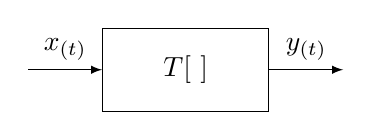
\begin{tikzpicture}[
            node distance=2cm,
            >=latex
            ]

            \node [coordinate] (input) {};
            \node [draw, rectangle,right of = input, minimum height=3em, minimum width=6em] (block) {$T[\ ]$};
            \node [coordinate, right of = block] (output) {};
            
            \draw[draw,->] (input) -- node[above]{$x_{(t)}$} (block);
            \draw[->] (block) -- node[above]{$y_{(t)}$} (output);
        \end{tikzpicture}    
    \label{Def sistema monodimensionale}
    \end{figure}
    Il sistema applica la trasformazione $T[\ ]: y_{(t)} = T[x_{(t)}]$ in gemerale \\ $y_{(t)} = T[x_{(\alpha)},t]$. 
    \subsection{Propietá dei Sistemi Lineari Tempo Invarianti (LTI)}
        \begin{itemize}
            \item {Linearitá:
                \[
                    x_{(t)} = ax_{1(t)}+bx_{2(t)} \overset{T[\ ]}{\Rightarrow} y_{(t)} = aT[x_{1(t)}]+b T[x_{2(t)}]
                \]
                Oppure separando la variabile del tempo:
                \[
                    x_{(t)} = ax_{1(t)}+bx_{2(t)} \overset{T[\ ]}{\Rightarrow} y_{(t)} = aT[x_{1(\alpha)},t]+b T[x_{2(\alpha)},t]
                \]
                É il principio di linearitá o sovrapposizione degli effetti visto a elettrotecnica.
            }\label{SM Linearita}
            \item {Stazionarietá:
                \[
                    y_{(t)} = T[x_{(t)}] \rightarrow y_{(t-t_0)} = T[x_{(t-t_0)}]  
                \]
            }\label{SM Stazionarieta}
            \item {Causalitá:
                \[
                    y_{(t)} = T[x_{(\alpha)},\alpha\leq t]
                \]
                L'uscita all'istante $t$ dipende dall'ingresso ad instanti precedenti o al piú uguali a $t$, si basa su valori precendenti a 
                $t$ non puó prevedere il futuro. Ne derivano 2 distinzioni di trasformazioni:
                \begin{itemize}
                    \item Real Time: necessariamente causale (é nel presente)
                    \item Virtual time: Causale o Non Causale (es. ho tutto un file al quale posso prevedere i bit o frame successivi per applicarne un post-processing)
                \end{itemize}
            }\label{SM Causalita}
            \item {Stabilitá BIBO:
                Se il segnale $x_{(t)}$ ha ampiezza limitata $\rightarrow$ l'uscita ha ampiezza limitata:
                    \[
                        |x_{(t)}|\leq M \rightarrow |y_{(t)}|\leq K 
                    \]
            }\label{SM Stabilita BIBO}
            \item {Invertibilitá:
                \[
                    y_{(t)} = T[x_{(\alpha)},t] \overset{\text{Se} \exists}{\Rightarrow} x_{(t)} = T^{-1}[y_{(\alpha)},t]
                \]
            }\label{SM Invertibilita}
            \item {Memoria:
                Un sistema é:
                \begin{itemize}
                    \item {Senza memoria: se $y_{(t)} = T[x_{(\alpha)},\alpha=t]$}
                    \item {Con Memoria: $y_{(t)} =\int_{-\infty}^{t}x_{(\alpha)} d\alpha$ l'uscita all'istante $t$ dipende anche da valori dell'ingresso 
                          ad istanti diversi da $t$. Nota bene é l'integrale di convoluzione di $x_{(t)} \otimes u_{(t)}$ 
                    }
                \end{itemize}
            }\label{SM Memoria}
        \end{itemize}
    \subsection{Propietá dei Sistemi Lineari Stazionari (SLS)}
        Sono sistemi che godono delle propietá di Linearitá \ref{SM Linearita} e di Stazionarietá \ref*{SM Stazionarieta}:
        \begin{figure}[H]
            \centering 
            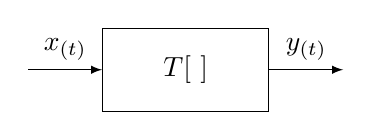
\begin{tikzpicture}[
                node distance=2cm,
                >=latex
                ]

                \node [coordinate] (input) {};
                \node [draw, rectangle,right of = input, minimum height=3em, minimum width=6em] (block) {$T[\ ]$};
                \node [coordinate, right of = block] (output) {};
                
                \draw[draw,->] (input) -- node[above]{$x_{(t)}$} (block);
                \draw[->] (block) -- node[above]{$y_{(t)}$} (output);
            \end{tikzpicture}    
        \label{Def SLS}
        \end{figure}  
        Troviamo la relazione tra ingresso e uscita:
        \begin{align}
            y_{(t)} &= T[x_{(\alpha)},t] =T[x_{(t)}] = T[x_{(t)} \otimes \delta_{(t)}] = T[\int_{-\infty}^{\infty}x_{(\alpha)}\delta_{(t-\alpha)}d\alpha]\nonumber \\        
                    &\overset{\ref*{SM Linearita}}{\Rightarrow} \underset{(\alpha)}{\int_{-\infty}^{\infty}}\underset{(t)}{T}[x_{(\alpha)}\delta_{(t-\alpha)}]d\alpha =\underset{(\alpha)}{\int_{-\infty}^{\infty}}x_{(\alpha)}\underset{(t)}{T}[\delta_{(t-\alpha)}]d\alpha\nonumber         
        \end{align}  
        Definiamo la trasformata nota del $\delta_{(t)}$:
        \begin{figure}[H]
            \centering 
            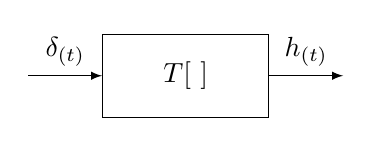
\begin{tikzpicture}[
                node distance=2cm,
                >=latex
                ]

                \node [coordinate] (input) {};
                \node [draw, rectangle,right of = input, minimum height=3em, minimum width=6em] (block) {$T[\ ]$};
                \node [coordinate, right of = block] (output) {};
                
                \draw[draw,->] (input) -- node[above]{$\delta_{(t)}$} (block);
                \draw[->] (block) -- node[above]{$h_{(t)}$} (output);
            \end{tikzpicture}    
        \label{Def impulso}
        \end{figure}
        Sollecitando il sistema con una Delta di Dirac ho la sua risposta impulsiva\index{Risposta Impulsiva}. Nel caso dei sistemi $SLS$ l'impulso
        in uscita caratterizza completamente il sistema. Nel nostro caso $T[\delta_{(t-\alpha)}]$ non é altro che una traslazione della $T[\delta_{(t)}]$ per la 
        Stazionarietá \ref*{SM Stazionarieta}: 
        \[
            y_{(t)} =\int_{-\infty}^{\infty}x_{(\alpha)}h_{(t-\alpha)}d\alpha = x_{(t)}\otimes h_{(t)} 
        \]
        La trasformata del sistema dipende solo dalla $h_{(t)}$. Passando al dominio della frequenza per la propietá della convoluzione \ref{Convoluzione}:
        \[
            y_{(t)} =X_{(f)}\otimes H_{(f)} 
        \]
        Dove$H_{(f)} = TCF[h_{(t)}] = \int_{-\infty}^{\infty} h_{(t)}e^{-j2\pi ft}$ é la risposta in frequenza del sistema $SLS$. Esistono vari modi
        per calcolare $h_{(t)}$:
        \begin{itemize}
            \item {
                
            }
        \end{itemize}
    \subsection{Risposta di un sistema causale e risposta impulsiva}
    
    \section{Trasformata Discreta di Fourier}
    Si definisce Trasformata Discreta di Fourier:
    \begin{gather}
        x_{[nT]} \overunderset{TDF}{ATDF}{\rightleftharpoons} \overline{X}_{(f)} \nonumber \\
        \overline{X}_{(f)} \in \mathbb{C}: \begin{cases}
            \left| \overline{X}_{(f)} \right| \nonumber \\
            \angle \overline{X}_{(f)} \nonumber
        \end{cases} \text{é una funzione periodica di periodo }\frac{1}{T}\nonumber  
    \end{gather}
    \subsubsection{Equazione di Analisi - $TDF$} \label{TDF}
        \[
            \overline{X}_{(f)} = \sum_{n=-\infty}^{\infty} x_{[nT]}e^{-j2\pi fnT}
        \]
    \subsubsection{Equazione di Sintesi - $ATDF$} \label{ATDF}
        \[
            x_{[nT]} = \frac{1}{2\pi} \int_{2\pi} \overline{X}_{(f)}e^{-j2\pi fnT} df
        \]
    \subsubsection{Trasformata di $\delta_{[n]}$}\label{tdf sequenza di delta}
        \begin{gather}
            \sum_{n=-\infty}^{\infty}\delta_{(t-nT)} \overset{\ref{prima formula di poisson}}{=} \frac{1}{T} \sum_{k=-\infty}^{\infty} \Delta_{(\frac{k}{T})}e^{-j2\pi \frac{k}{T}t} \overset{\Delta \text{ costante}}{=} \frac{1}{T} \sum_{k=-\infty}^{\infty} e^{-j2\pi \frac{k}{T}t} \nonumber \\
            \Downarrow TCF\nonumber \\
            \sum_{n=-\infty}^{\infty}e^{-j2\pi fnT} = \frac{1}{T} \sum_{k=-\infty}^{\infty} \delta_{(f-\frac{k}{T})}\nonumber
        \end{gather}
        Applicando il ritardo:
        \[
            \sum_{n=-\infty}^{\infty}e^{-j2\pi (f-\nu)nT} = \frac{1}{T} \sum_{k=-\infty}^{\infty} \delta_{((f-\nu)-\frac{k}{T})}
        \]
    \subsubsection{Relazione tra $TCF$ e $TDF$}\label{Relazione tra $TCF$ e $TDF$}
        \begin{align}
            \overline{X}_{(f)} &= \sum_{n=-\infty}^{\infty} x_{[nT]}e^{-j2\pi fnT} = \sum_{n=-\infty}^{\infty} \underset{(\nu)}{\int_{-\infty}^{\infty}} X_{(\nu)} e^{-j2\pi \nu nT} d\nu e^{-j2\pi fnT} \nonumber \\
                               &= \underset{(\nu)}{\int_{-\infty}^{\infty}} X_{(\nu)} \sum_{n=-\infty}^{\infty} e^{-j2\pi \nu nT} e^{-j2\pi fnT} d\nu \overset{\ref{tdf sequenza di delta}}{=} \underset{(\nu)}{\int_{-\infty}^{\infty}} X_{(\nu)} \sum_{n=-\infty}^{\infty} \frac{1}{T} \delta_{((f-\nu)-\frac{k}{T})} d\nu  \nonumber \\
                               &\overset{\ref{Propietá del Delta di Dirac}:\text{paritá}}{=} \underset{(\nu)}{\int_{-\infty}^{\infty}} X_{(\nu)} \frac{1}{T} \sum_{n=-\infty}^{\infty}  \delta_{(\nu-(f-\frac{k}{T}))} d\nu = \frac{1}{T} \sum_{n=-\infty}^{\infty} \underset{(\nu)}{\int_{-\infty}^{\infty}} X_{(\nu)} \delta_{(\nu-(f-\frac{k}{T}))} d\nu  \nonumber \\
                               &\overset{\ref{Propietá del Delta di Dirac}:\text{campionatrice}}{=}  \frac{1}{T} \sum_{n=-\infty}^{\infty} X_{(f-\frac{k}{T})} \nonumber
        \end{align}
        quindi la $TDF$ si ottiene periodicizzando la $TCF$ con periodo $\frac{1}{T}$:
        \[
            \overline{X}_{(f)} = \frac{1}{T} \sum_{n=-\infty}^{\infty} X_{(f-\frac{k}{T})} 
        \] 
        \begin{figure}[H]
            \centering
            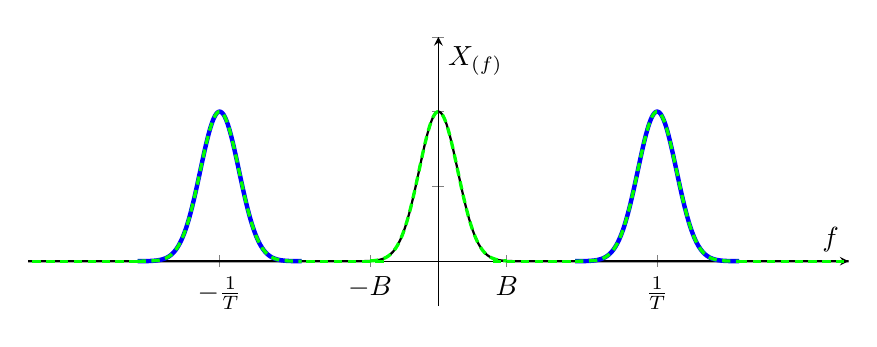
\begin{tikzpicture}
                \begin{axis}[
                    domain=-15:15,
                    samples=200,
                    axis lines=middle,
                    xlabel=$f$,
                    ylabel=$X_{(f)}$,
                    ymin=-0.3,
                    ymax=1.5,
                    xtick={-8,-2.5,2.5,8},
                    xticklabels={$-\frac{1}{T}$,$-B$,$B$,$\frac{1}{T}$},
                    ytick={},
                    yticklabels={},
                    width=12cm,
                    height=5cm
                ]

                \addplot [thick,black, samples = 800] {exp(-x^2)};
                \addplot [ultra thick,blue, domain = -11:-5, samples = 800] {exp(-(x+8)^2)};
                \addplot [ultra thick,blue, domain = 5:11, samples = 800] {exp(-(x-8)^2)};

                \addplot [densely dashed,very thick,green, domain = -2.5:2.5, samples = 900] {exp(-x^2)};
                \addplot [densely dashed,very thick,green, domain = -11:-5, samples = 800] {exp(-(x+8)^2)};
                \addplot [densely dashed,very thick,green, domain = 5:11, samples = 800] {exp(-(x-8)^2)};
                \addplot [densely dashed,very thick,green] coordinates{(-11,0)(-15,0)};
                \addplot [densely dashed,very thick,green] coordinates{(11,0)(15,0)};
                \addplot [densely dashed,very thick,green] coordinates{(-2,0)(-5,0)};
                \addplot [densely dashed,very thick,green] coordinates{(2,0)(5,0)};

                \end{axis}
            \end{tikzpicture}
            \caption{${\color{black} X_{(f)}}$,${\color{blue} X_{(f-\frac{k}{T})}}$,${\color{green} \overline{X}_{(f)}}$}
            \label{fig:relazione tdf tcf}
        \end{figure}
    \subsection{Teorema del Campionamento - Nyquist Shannon}\label{Teorema del Campionamento - Nyquist Shannon}
        \begin{figure}[H]
            \centering
                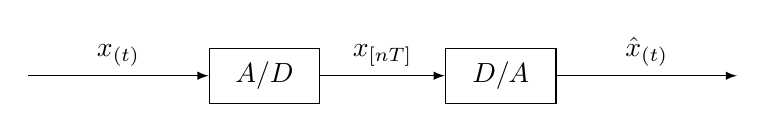
\begin{tikzpicture}[
                        node distance=3cm,
                        >=latex
                    ]
                    % Blocks
                    \node [coordinate] (input) {};
                    \node [rectangle, draw,minimum height=2em, minimum width=4em,right of=input] (AD) {$A/D$};
                    \node [rectangle, draw,minimum height=2em, minimum width=4em,right of=AD] (DA) {$D/A$};
                    \node [coordinate,right of=DA] (output) {};
                
                    % Connections
                    \draw [->] (input) --node[above]{$x_{(t)}$} (AD);
                    \draw [->] (AD) --node[above]{$x_{[nT]}$} (DA);
                    \draw [->] (DA) --node[above]{$\hat{x}_{(t)}$} (output);
                \end{tikzpicture}    
            \label{fig:Sistema di campionamento e ricostruzione}
            \caption{Esempio sistema campionamento e ricostruzione}
        \end{figure}
        \begin{itemize}
            \item {
                A/D: Campionatore, converte da analogico a discreto.
            }
            \item {
                A/D: interpolatore o filtro $p$, converte da discreto a analogico.
            }
        \end{itemize}
        Il nostro obbiettivo é dimensionare T e l'interpolatore in modo tale da poter ricostruire il segnale $\hat{x}:\ \hat{x} =x$.
        \paragraph{Dimensioniamo l'$A/D$:} Riprendiamo la relazione tra $TDF$ e $TCF$:
        \begin{figure}[H]
            \centering
            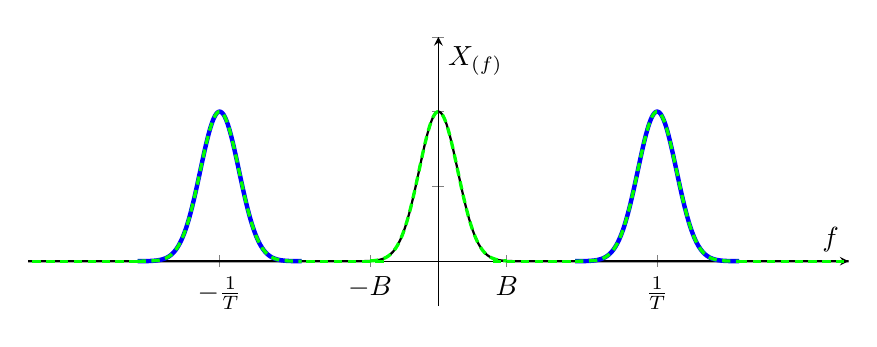
\begin{tikzpicture}
                \begin{axis}[
                    domain=-15:15,
                    samples=200,
                    axis lines=middle,
                    xlabel=$f$,
                    ylabel=$X_{(f)}$,
                    ymin=-0.3,
                    ymax=1.5,
                    xtick={-8,-2.5,2.5,8},
                    xticklabels={$-\frac{1}{T}$,$-B$,$B$,$\frac{1}{T}$},
                    ytick={},
                    yticklabels={},
                    width=12cm,
                    height=5cm
                ]
                
                \addplot [thick,black, samples = 800] {exp(-x^2)};
                \addplot [ultra thick,blue, domain = -11:-5, samples = 800] {exp(-(x+8)^2)};
                \addplot [ultra thick,blue, domain = 5:11, samples = 800] {exp(-(x-8)^2)};

                \addplot [densely dashed,very thick,green, domain = -2.5:2.5, samples = 900] {exp(-x^2)};
                \addplot [densely dashed,very thick,green, domain = -11:-5, samples = 800] {exp(-(x+8)^2)};
                \addplot [densely dashed,very thick,green, domain = 5:11, samples = 800] {exp(-(x-8)^2)};
                \addplot [densely dashed,very thick,green] coordinates{(-11,0)(-15,0)};
                \addplot [densely dashed,very thick,green] coordinates{(11,0)(15,0)};
                \addplot [densely dashed,very thick,green] coordinates{(-2,0)(-5,0)};
                \addplot [densely dashed,very thick,green] coordinates{(2,0)(5,0)};

                \end{axis}
            \end{tikzpicture}
            \caption{${\color{black} X_{(f)}}$,${\color{blue} X_{(f-\frac{k}{T})}}$,${\color{green} \overline{X}_{(f)} = \frac{1}{T}\sum_{k=-\infty}^{\infty}X_{(f-\frac{k}{T})}}$}
            \label{fig:relazione tdf tcf campionamento f 2B}
        \end{figure}

        abbiamo trovato che la $TDF$  non é altro che la periodicizzazione della $TCF$ con periodo $\frac{1}{T}$: se $\frac{1}{T}\geq 2B$
        il grafico ${\color{blue} X_{(f-\frac{k}{T})}}$ sono copie distinte non distorte e periodicizzate di $X_{(f)}$ da cui con un Filtro Passa-Basso \ref{Filtro Passa Basso di banda B - Low Pass Filter (LP)} 
        possiamo ricostruire il segnale. Se scegliessi $\frac{1}{T}<2B$:
        \begin{figure}[H]
            \centering
            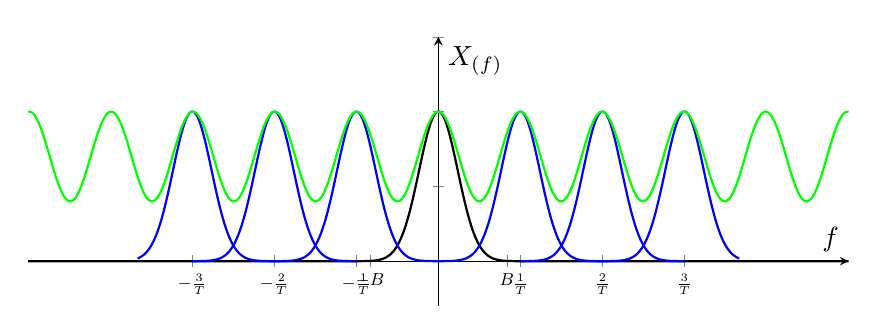
\begin{tikzpicture}
                \begin{axis}[
                    domain=-15:15,
                    samples=200,
                    axis lines=middle,
                    xlabel=$f$,
                    ylabel=$X_{(f)}$,
                    ymin=-0.3,
                    ymax=1.5,
                    xtick={-9,-6,-3,-2.5,2.5,3,9,6},
                    xticklabels={$-\frac{3}{T}$,$-\frac{2}{T}$,$-\frac{1}{T}$,$-B$,$B$,$\frac{1}{T}$,$\frac{3}{T}$,$\frac{2}{T}$,},
                    xticklabel style={font = \small,scale = 0.7},
                    ytick={},
                    yticklabels={},
                    width=12cm,
                    height=5cm
                ]
                
                \addplot [thick,black, samples = 800] {exp(-x^2)};
                \addplot [thick,blue, domain = -6:0, samples = 800] {exp(-(x+3)^2)};
                \addplot [thick,blue, domain = 0:6, samples = 800] {exp(-(x-3)^2)};

                \addplot [thick,blue, domain = -9:-3, samples = 800] {exp(-(x+6)^2)};
                \addplot [thick,blue, domain = 3:9, samples = 800] {exp(-(x-6)^2)};

                \addplot [thick,blue, domain = -11:-6, samples = 800] {exp(-(x+9)^2)};
                \addplot [thick,blue, domain = 6:11, samples = 800] {exp(-(x-9)^2)};

                \addplot [thick,green , samples = 800] {0.3*cos(deg(2.1*x))+0.7};

                \end{axis}
            \end{tikzpicture}
            \caption{${\color{black} X_{(f)}}$,${\color{blue} X_{(f-\frac{k}{T})}}$,${\color{green} \overline{X}_{(f)} = \frac{1}{T}\sum_{k=-\infty}^{\infty}X_{(f-\frac{k}{T})}}$}
            \label{fig:relazione tdf tcf campionamento f sbagliata}
        \end{figure}
        ho sovrapposizione delle copie di $X_{(f)}$ é il fenomeno di Aliasing: ho sovrapposizione di segnali che alterano il segnale originale. 
        In entrambi i casi ci troviamo in condizione di un segnale a banda limitata, nel tempo rappresenta un segnale illimitato.
        \paragraph{Dimensioniamo il $D/A$:}
        Partiamo dalla relazione di $\hat{x}$:
        \[
            \hat{x} = \sum_{n=-\infty}^{\infty}x_{[nT]}p_{(t-nT)},\ p\text{ interpolatore}
        \]
        Il segnale di uscita dal sistema dipende non solo dal periodo di campionamento $\frac{1}{T}$ ma anche dall'interpolatore che utilizziamo:
        \begin{itemize}
            \item {Interpolatore a mantenimento: mantiene il valore del segnale $x_{[nT]}$ per un periodo $T$
                \begin{figure}[H]
                    \centering
                    \begin{tikzpicture}
                        \begin{axis}[
                            domain=-5:5,
                            samples=200,
                            axis lines=middle,
                            xlabel=$t$,
                            ylabel=$p_{(t)}$,
                            ymin=-0.3,
                            ymax=5,
                            xmax=5,
                            xtick={3},
                            xticklabels={$T$},
                            ytick={1.5},
                            width=9cm,
                            height=4.5cm
                        ]
                        %x(t)
                        \addplot [const plot, thick, orange] coordinates{(0,0)(0,1.5)(3,1.5)(3,0)};
                        %Colors
                        \end{axis}
                    \end{tikzpicture}
                    \caption{Interpolatore a mantenimento}
                    \label{fig:interpolatore a mantenimento}
                \end{figure}
                \begin{figure}[H]
                    \centering
                    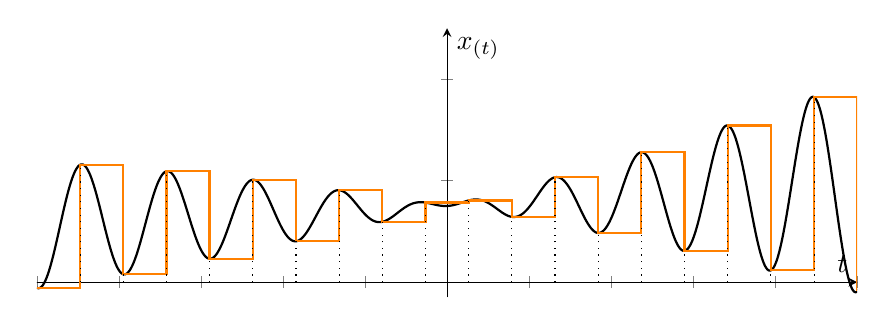
\begin{tikzpicture}
                        \begin{axis}[
                            domain=-5:5,
                            samples=200,
                            axis lines=middle,
                            xlabel=$t$,
                            ylabel=$x_{(t)}$,
                            ymin=-0.3,
                            ymax=5,
                            xtick={},
                            xticklabels={},
                            ytick={},
                            yticklabels={},
                            width=12cm,
                            height=5cm
                        ]
                        %x(t)
                        \addplot [thick,black, samples = 1000] {(x/3*sin(deg(6*x))+1.5)*((x/20)+1)};
                        \addplot [const plot,thick,orange, samples = 20] {(x/3*sin(deg(6*x))+1.5)*((x/20)+1)};
                        \addplot+ [ycomb, mark = none, dotted, black, samples = 20] {(x/3*sin(deg(6*x))+1.5)*((x/20)+1)};
                        %Colors
                        \end{axis}
                    \end{tikzpicture}
                    \caption{$x_{(t)}$,{\color{orange}$\hat{x} = \sum_{n=-\infty}^{\infty}x_{[nT]}p_{(t-nT)}$}}
                    \label{fig:x con interpolatore a mantenimento}
                \end{figure}
            }
            \item {Interpolatore Lineare: incrementa linearmente il valore di $\hat{x}$
                \begin{figure}[H]
                    \centering
                    \begin{tikzpicture}
                        \begin{axis}[
                            domain=-5:5,
                            samples=200,
                            axis lines=middle,
                            xlabel=$t$,
                            ylabel=$p_{(t)}$,
                            ymin=0.3,
                            xmin=-5,
                            ymax=5,
                            xmax=5,
                            xtick={-1.7,1.7},
                            xticklabels={$-\frac{T}{2}$,$\frac{T}{2}$},
                            ytick={2},
                            yticklabels={$1$},
                            width=9cm,
                            height=5cm
                        ]
                        \addplot [sharp plot,thick,orange] coordinates{(-2,0)(0,2)(2,0)};
                        \end{axis}
                    \end{tikzpicture}
                    \caption{Interpolatore Lineare}
                    \label{fig:interpolatore Lineare}
                \end{figure}
                \begin{figure}[H]
                    \centering
                    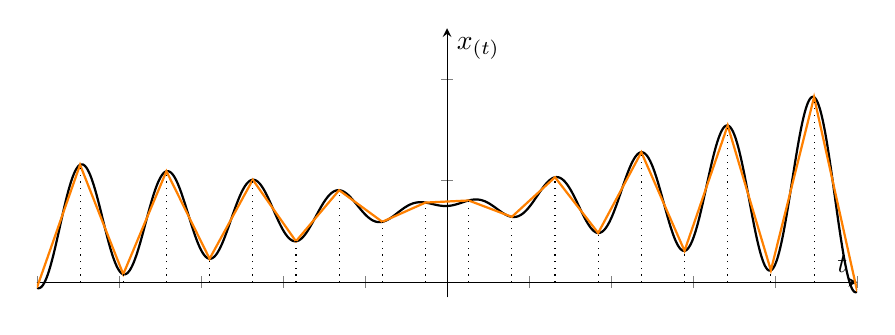
\begin{tikzpicture}
                        \begin{axis}[
                            domain=-5:5,
                            samples=200,
                            axis lines=middle,
                            xlabel=$t$,
                            ylabel=$x_{(t)}$,
                            ymin=-0.3,
                            ymax=5,
                            xtick={},
                            xticklabels={},
                            ytick={},
                            yticklabels={},
                            width=12cm,
                            height=5cm
                        ]
                        
                        \addplot [thick,black, samples = 1000] {(x/3*sin(deg(6*x))+1.5)*((x/20)+1)};
                        \addplot [sharp plot,thick,orange, samples = 20] {(x/3*sin(deg(6*x))+1.5)*((x/20)+1)};
                        \addplot+ [ycomb, mark = none, dotted, black, samples = 20] {(x/3*sin(deg(6*x))+1.5)*((x/20)+1)};
                        \end{axis}
                    \end{tikzpicture}
                    \caption{$x_{(t)}$,{\color{orange}$\hat{x} = \sum_{n=-\infty}^{\infty}x_{[nT]}p_{(t-nT)}$}}
                    \label{fig:x con interpolatore Lineare}
                \end{figure}
            }
        \end{itemize}
        Passiamo alla frequenza:
        \[
            \hat{x} = \sum_{n=-\infty}^{\infty}x_{[nT]}p_{(t-nT)} \overset{TCF}{\rightleftharpoons} \hat{X}_{(f)} = \sum_{n=-\infty}^{\infty}x_{[nT]}P_{(f)}e^{-j2\pi fnT}
        \]
        \begin{gather}
            \hat{X}_{(f)} = P_{(f)}\sum_{n=-\infty}^{\infty}x_{[nT]}e^{-j2\pi fnT} = P_{(f)}\overline{X}_{(f)} \nonumber \\
            Se\ \hat{x}=x\ anche\ \hat{X}_{(f)} = X_{(f)}\nonumber \\
            \Downarrow \ref{Relazione tra $TCF$ e $TDF$} \nonumber \\
            X_{(f)} \overset{!}{=} P_{(f)}\frac{1}{T}\sum_{k=-\infty}^{\infty}X_{(f-\frac{k}{T})} \nonumber
        \end{gather}
        dobbiamo dimensionare $P_{(f)}$ in modo tale da rendere vera $\hat{X}_{(f)} = X_{(f)}$
        \begin{figure}[H]
            \centering
            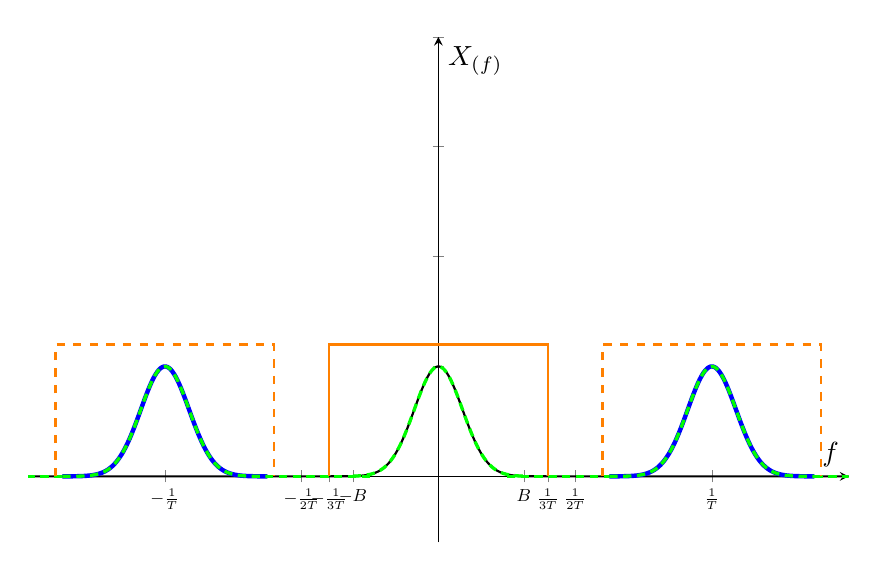
\begin{tikzpicture}
                \begin{axis}[
                    domain=-12:12,
                    samples=200,
                    axis lines=middle,
                    xlabel=$f$,
                    ylabel=$X_{(f)}$,
                    ymin=-0.3,
                    ymax=2,
                    xmax=12,
                    xmin=-12,
                    xtick={-8,-4,-3.2,-2.5,2.5,3.2,4,8},
                    xticklabels={$-\frac{1}{T}$,$-\frac{1}{2T}$,$-\frac{1}{3T}$,$-B$,$B$,$\frac{1}{3T}$,$\frac{1}{2T}$,$\frac{1}{T}$},
                    xticklabel style={font = \small,scale = 0.7},
                    ytick={},
                    yticklabels={},
                    width=12cm,
                    height=8cm 
                ]
                
                \addplot [thick,black, samples = 800] {0.5*exp(-x^2)};
                \addplot [ultra thick,blue, domain = -11:-5, samples = 800] {0.5*exp(-(x+8)^2)};
                \addplot [ultra thick,blue, domain = 5:11, samples = 800] {0.5*exp(-(x-8)^2)};

                \addplot [densely dashed,very thick,green, domain = -2.5:2.5, samples = 900] {0.5*exp(-x^2)};
                \addplot [densely dashed,very thick,green, domain = -11:-5, samples = 800] {0.5*exp(-(x+8)^2)};
                \addplot [densely dashed,very thick,green, domain = 5:11, samples = 800] {0.5*exp(-(x-8)^2)};
                
                \addplot [densely dashed,very thick,green] coordinates{(-11,0)(-15,0)};
                \addplot [densely dashed,very thick,green] coordinates{(11,0)(15,0)};
                \addplot [densely dashed,very thick,green] coordinates{(-2,0)(-5,0)};
                \addplot [densely dashed,very thick,green] coordinates{(2,0)(5,0)};

                \addplot [const plot, thick,orange] coordinates{(-3.2,0)(-3.2,0.6)(3.2,0.6)(3.2,0)};
                \addplot [const plot, dashed ,thick,orange] coordinates{(-11.2,0)(-11.2,0.6)(-4.8,0.6)(-4.8,0)};
                \addplot [const plot, dashed ,thick,orange] coordinates{(4.8,0)(4.8,0.6)(11.2,0.6)(11.2,0)};

                \end{axis}
            \end{tikzpicture}
            \caption{${\color{black} X_{(f)}}$,${\color{blue} X_{(f-\frac{k}{T})}}$,${\color{orange} P_{(f)}}$}
            \label{fig:tdf tcf dimansionamento interpolatore}
        \end{figure}
        Utilizziamo un filtro passa basso che abbia una durata in banda maggiore di $2B$ ma minore di $\frac{1}{2T}$  per lasciarci un pochino di margine e evitare  di prendere 
        la copia del segnale successivo/precedente ($2B<T_r\leq\frac{1}{2T_s}$): prendiamo una durata $\frac{1}{2T_s}>2B$
        \[
            P_{(f)} = T rect\left(\frac{f}{2\frac{1}{2T}}\right)= T rect\left(fT\right) \overset{TCF}{\leftrightharpoons} p_{(t)} = \frac{T}{T}sinc\left(\frac{t}{T}\right)
        \]
        
        \paragraph{Interpolatore a seno cardinale:} Si utilizza un interpolatore a seno cardinale
            \begin{figure}[H] $he$
                \centering
                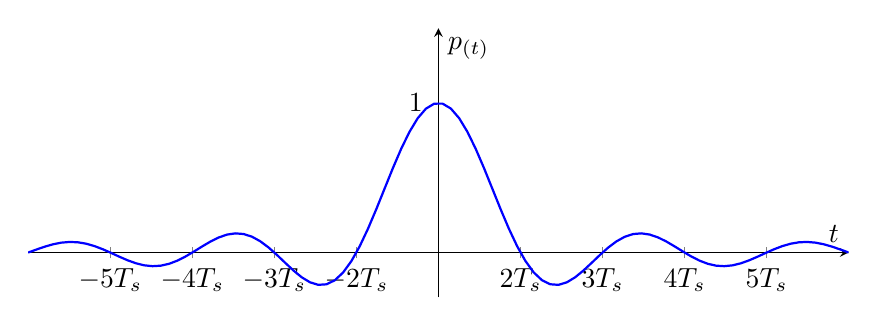
\begin{tikzpicture}
                    \begin{axis}[
                        domain=-5:5,
                        samples=200,
                        axis lines=middle,
                        xlabel=$t$,
                        ylabel=$p_{(t)}$,
                        ymin=-0.3,
                        ymax=1.5,
                        xtick={-4,-3,-2,-1,-0,0,0,1,2,3,4},
                        xticklabels={$-5T_s$,$-4T_s$,$-3T_s$,$-2T_s$,$-T_s$,$0$,$T_s$,$2T_s$,$3T_s$,$4T_s$,$5T_s$},
                        ytick={1},
                        yticklabels={$1$},
                        width=12cm,
                        height=5cm
                    ]
                    %x(t)
                    \addplot [blue, thick, samples = 100] {sin(deg(x*pi))/(x*pi)};
                    \end{axis}
                \end{tikzpicture}
                \caption{Interpolatore a seno cardinale}
                \label{fig:interpolatore a seno cardinale}
            \end{figure}
            \begin{figure}[H]
                \centering
                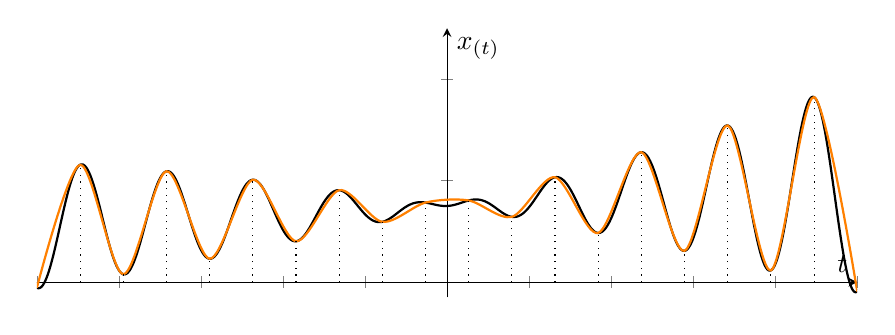
\begin{tikzpicture}
                    \begin{axis}[
                        domain=-5:5,
                        samples=200,
                        axis lines=middle,
                        xlabel=$t$,
                        ylabel=$x_{(t)}$,
                        ymin=-0.3,
                        ymax=5,
                        xtick={},
                        xticklabels={},
                        ytick={},
                        yticklabels={},
                        width=12cm,
                        height=5cm
                    ]
                    \addplot [thick,black, samples = 1000] {(x/3*sin(deg(6*x))+1.5)*((x/20)+1)};
                    \addplot [smooth,thick,orange, samples = 20] {(x/3*sin(deg(6*x))+1.5)*((x/20)+1)};
                    \addplot+ [ycomb, mark = none, dotted, black, samples = 20] {(x/3*sin(deg(6*x))+1.5)*((x/20)+1)};

                    \end{axis}
                \end{tikzpicture}
                \caption{$x_{(t)}$,{\color{orange}$\hat{x} = \sum_{n=-\infty}^{\infty}x_{[nT]}p_{(t-nT)}$}}
                \label{fig:x con interpolatore a seno cardinale}
            \end{figure}
            l'interpolatore a seno cardinale non é causale: essendo delle $sinc$ a ogni campionamento, non posso conoscere il peso delle $sinc$ 
            dei valori della sequenza successivi. Se opero non Real Time (Virtuale), invece ho infiniti campioni a cui posso attingere: Risolvo entrambi i 
            problemi troncando la $sinc$ e spostandola a dx, ma per troncarla sto moltiplicando una $sinc$ per una $rect$ nel tempo, passando alla frequenza 
            la funzione limitata nel tempo diventa illimitata in frequenza andando a influenzare anche le repliche successive.


        
        \paragraph{Teorema del Campionamento:} Dato un segnale analogico $x_{(t)}$ la cui banda di frequenze sia limitata e dato $c\in \mathbb{Z}$,
        il segnale $x_{(t)}$ puó essere univocamente ricostruito a partire dai suoi campioni $x_{[nT]}$ presi a frequenza (o periodo) $f_s = \frac{1}{T}$ se 
        $f_s = \frac{1}{T} \geq 2B$ mediante:
        \[
            x_{(t)} = \sum_{n=-\infty}^{\infty} x_{[nT]}sinc\left(\frac{t}{T}-n\right) 
        \]
        Criticitá
        \begin{itemize}
            \item {Segnale a banda limitata}
            \item {Interpolatore dimensionato}
        \end{itemize}
        Osservazioni: Se utilizzassi un filtro con durata $\frac{1}{T}>>2B$ prenderei tantissimi campioni che
        non servono per ricostruire meglio il segnale: dagli esempi di matlab possiamo vedere che ci basta anche solo un periodo uguale a $2B$.\\
        Esempio:
        \[
            B = 10KHz,\ 2B = 20KHz,\ \text{Durata filtro} = 25KHz\ ho\ 5KHz\text{ di margine}
        \]
        Esempio:$f_s = \frac{1}{T} = 2B,\ p_{(t)}=sinc(2Bt)$
        \begin{gather}
                \hat{x}_{(t)} = \sum_{n=-\infty}^{\infty} x_{[nT]}sinc\left(2Bt_0 -n\right) \nonumber \\
                \hat{x}_{(t_0)} = \sum_{n=-\infty}^{\infty} x_{[nT]}sinc\left(2Bt_0 -n\right) \nonumber
        \end{gather}
        $\hat{x}_{(t_0)}$ dipende dal contributo di tutte le $sinc$ anche dei valori successivi, per questo si pone il problema del filtro causale. 
        \begin{figure}[H]
            \centering
            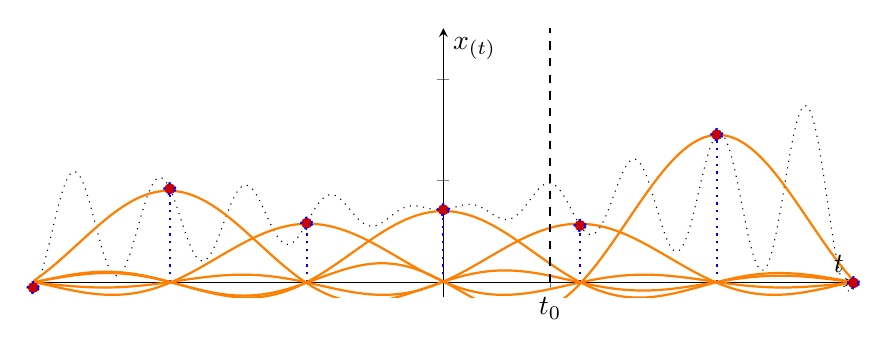
\begin{tikzpicture}
                \begin{axis}[
                    domain=-5:5,
                    samples=200,
                    axis lines=middle,
                    xlabel=$t$,
                    ylabel=$x_{(t)}$,
                    ymin=-0.3,
                    ymax=5,
                    xtick={1.3},
                    xticklabels={$t_0$},
                    ytick={},
                    yticklabels={},
                    width=12cm,
                    height=5cm
                ]
                % 0.53 periodo
                \addplot [thin,dotted,black, samples = 1000] {(x/3*sin(deg(6*(x-1)))+1.5)*(((x-1)/20)+1)};
                \addplot+ [ycomb, mark = *, dotted, blue,thick, samples = 7] {(x/3*sin(deg(6*(x-1)))+1.5)*(((x-1)/20)+1)};
                % Sinc x positive
                \addplot [orange, thick, samples = 500] {1.4*sin(deg((x)*pi*0.6))/((x)*pi*0.6)};
                \addplot [orange, thick, samples = 500] {1.15*sin(deg((x-1.65)*pi*0.6))/((x-1.65)*pi*0.6)};
                \addplot [orange, thick, samples = 500] {2.9*sin(deg((x-3.35)*pi*0.6))/((x-3.35)*pi*0.6)};
                % \addplot [orange, thick, samples = 500] {1.3*sin(deg((x-1.325)*pi*2))/((x-1.325)*pi*2)};
                % \addplot [orange, thick, samples = 500] {1.3*sin(deg((x-1.855)*pi*2))/((x-1.855)*pi*2)};
                % \addplot [orange, thick, samples = 500] {1.3*sin(deg((x-2.385)*pi*2))/((x-2.385)*pi*2)};
                % \addplot [orange, thick, samples = 500] {1.3*sin(deg((x-2.915)*pi*2))/((x-2.915)*pi*2)};
                % \addplot [orange, thick, samples = 500] {1.3*sin(deg((x-3.445)*pi*2))/((x-3.445)*pi*2)};
                % \addplot [orange, thick, samples = 500] {1.3*sin(deg((x-3.975)*pi*2))/((x-3.975)*pi*2)};
                % \addplot [orange, thick, samples = 500] {1.3*sin(deg((x-4.505)*pi*2))/((x-4.505)*pi*2)};
                % Sinc x negative
                \addplot [orange, thick, samples = 500] {1.15*sin(deg((x+1.65)*pi*0.6))/((x+1.65)*pi*0.6)};
                \addplot [orange, thick, samples = 500] {1.8*sin(deg((x+3.35)*pi*0.6))/((x+3.35)*pi*0.6)};
                % \addplot [orange, thick, samples = 500] {1.3*sin(deg((x+1.855)*pi*2))/((x+1.855)*pi*2)};
                % \addplot [orange, thick, samples = 500] {1.3*sin(deg((x+2.385)*pi*2))/((x+2.385)*pi*2)};
                % \addplot [orange, thick, samples = 500] {1.3*sin(deg((x+2.915)*pi*2))/((x+2.915)*pi*2)};
                % \addplot [orange, thick, samples = 500] {1.3*sin(deg((x+3.445)*pi*2))/((x+3.445)*pi*2)};
                % \addplot [orange, thick, samples = 500] {1.3*sin(deg((x+3.975)*pi*2))/((x+3.975)*pi*2)};
                % \addplot [orange, thick, samples = 500] {1.3*sin(deg((x+4.505)*pi*2))/((x+4.505)*pi*2)};
                \addplot [black, thick,dashed] coordinates{(1.3,0)(1.3,5)};
                \end{axis}
            \end{tikzpicture}
            \caption{$x_{(t)}$,{\color{orange}$\hat{x} = \sum_{n=-\infty}^{\infty}x_{[nT]}p_{(t-nT)}$}}
            \label{fig:Interpolatore seno cardinale}
        \end{figure}
        I passi in un sistema A/D/A sono:
        \begin{itemize}
            \item {Passo dal tempo in frequenza: $x_{(t)} \overset{TCF}{\rightleftharpoons} X_{(f)}$}.
            \item {Osservo la banda che occupa il segnale e scelgo $B$.}
            \item {Scelgo una frequenza (periodo) di campionamento $f_s$ e calcolo $x_{[nT]}$.}
            \item {Calcolo $\hat{x}$ con un interpolatore a seno cardinale,$sinc$}
        \end{itemize}

























    \section{Teoria della Probabilitá}
    \subsection{Introduzione}
        Perché abbiamo bisogno della teoria della probabilitá? Prendiamo un sistema di comunicazione:
        \begin{figure}[H]
            \centering
                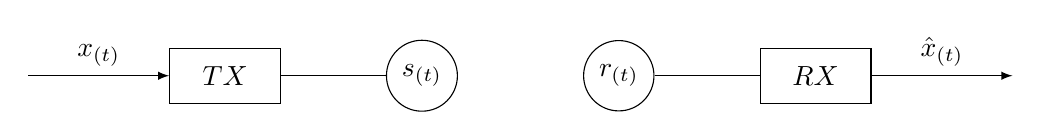
\begin{tikzpicture}[
                        node distance=2.5cm,
                        >=latex
                    ]
                    % Blocks
                    \node [coordinate] (input) {};
                    \node [rectangle, draw,minimum height=2em, minimum width=4em,right of=input] (TX) {$TX$};
                    \node [circle,draw,right of=TX] (TXant) {$s_{(t)}$};
                    \node [circle,draw,right of=TXant] (RXant) {$r_{(t)}$};
                    \node [rectangle, draw,minimum height=2em, minimum width=4em,right of=RXant] (RX) {$RX$};
                    \node [coordinate,right of=RX] (output) {};
                
                    % Connections
                    \draw [->] (input) --node[above]{$x_{(t)}$} (TX);
                    \draw [-] (TX) -- (TXant);
                    \draw [-] (RXant) -- (RX);
                    \draw [->] (RX) --node[above]{$\hat{x}_{(t)}$} (output);
                \end{tikzpicture}    
            \label{fig:Sistema di comunicazione}
            \caption{Esempio sistema di comunicazione}
        \end{figure}
        Analizziamo la parte di trasmissione $TX$:
        \begin{figure}[H]
            \centering
                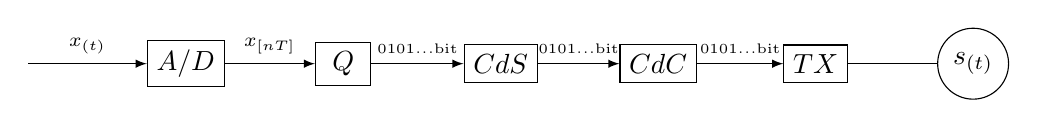
\begin{tikzpicture}[
                        node distance=2cm,
                        >=latex
                    ]
                    % Blocks
                    \node [coordinate] (input) {};
                    \node [rectangle, draw,minimum height=1em, minimum width=2em,right of=input] (AD) {$A/D$};
                    \node [rectangle, draw,minimum height=1em, minimum width=2em,right of=AD] (Q) {$Q$};
                    \node [rectangle, draw,minimum height=1em, minimum width=2em,right of=Q] (CS) {$CdS$};
                    \node [rectangle, draw,minimum height=1em, minimum width=2em,right of=CS] (CC) {$CdC$};
                    \node [rectangle, draw,minimum height=1em, minimum width=2em,right of=CC] (TX) {$TX$};
                    \node [circle,draw,right of=TX] (TXant) {$s_{(t)}$};
                
                    % Connections
                    \draw [->] (input) --node[above]{\scriptsize $x_{(t)}$} (AD);
                    \draw [->] (AD) --node[above]{\scriptsize$x_{[nT]}$} (Q);
                    \draw [->] (Q) --node[above]{\tiny$0101...$bit} (CS);
                    \draw [->] (CS) --node[above]{\tiny$0101...$bit} (CC);
                    \draw [->] (CC) --node[above]{\tiny$0101...$bit} (TX);
                    \draw [-] (TX) -- (TXant);
                \end{tikzpicture}    
            \label{fig:Sistema di comunicazione trasmettitore}
            \caption{Esempio sistema di trasmettitore}
        \end{figure}
        \begin{itemize}
            \item {Convertitore Analogico/Digitale ($A/D$): Campiona con frequenza $f_s$ e crea la sequenza $x_{[nT]}$.}
            \item {Quantizzatore ($Q$): Converte i valori della sequenza $x_{[nT]}$ in informazioni, bit. Ho sempre perdita di informazione a 
                questo livello, per quanti livelli di quantizzazione io metta il quantizzatore introdurrá sempre un'approssimazione. 
            }
            \item{Nei blocchi sotto elencati é dove entra in gioco la Teoria dei Codici, ci permettono di comprimere i dati e proteggerli dagli errori del canale:
                \begin{itemize}
                    \item {Codici di Sorgente ($CdS$): Comprimono i bit in ingresso dal quantizzatore eliminando la ridondanza.}
                    \item {Codifica di Canale ($CdC$): Aggiunge ridondanza ai dati da trasmettere per proteggere i dati dagli errori del canale.}
                \end{itemize}
            \item {Trasmettitore ($TX$):Si occupa di rendere il segnale trasmissibile sul canale di interesse e trasmettere il risultato $s_{(t)}$.}
            }
        \end{itemize}
        Analizziamo la parte di Ricezione $RX$:
        \begin{figure}[H]
            \centering
                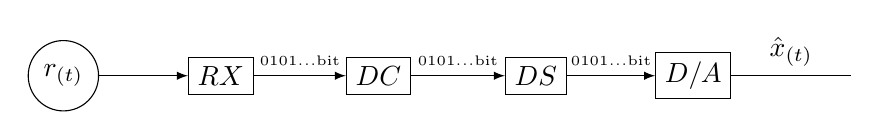
\begin{tikzpicture}[
                        node distance=2cm,
                        >=latex
                    ]
                    % Blocks
                    \node [circle,draw] (RXant) {$r_{(t)}$};
                    \node [rectangle, draw,minimum height=1em, minimum width=2em,right of=RXant] (RX) {$RX$};
                    \node [rectangle, draw,minimum height=1em, minimum width=2em,right of=RX] (DC) {$DC$};
                    \node [rectangle, draw,minimum height=1em, minimum width=2em,right of=DC] (DS) {$DS$};
                    \node [rectangle, draw,minimum height=1em, minimum width=2em,right of=DS] (DA) {$D/A$};
                    \node [coordinate,right of = DA] (output) {};
                
                    % Connections
                    \draw [->] (RXant) --node[above]{} (RX);
                    \draw [->] (RX) --node[above]{\tiny$0101...$bit} (DC);
                    \draw [->] (DC) --node[above]{\tiny$0101...$bit} (DS);
                    \draw [->] (DS) --node[above]{\tiny$0101...$bit} (DA);
                    \draw [-] (DA) --node[above]{$\hat{x}_{(t)}$} (output);
                \end{tikzpicture}    
            \label{fig:Sistema di comunicazione ricevitore}
            \caption{Esempio sistema di ricevitore}
        \end{figure}
        \begin{itemize}
            \item {RIcevitore ($RX$): Si occupa della ricezione del segnale trasmesso $r_{(t)}$.}
            \item{La Teoria dei Codici si applica anche in ricezione per la decodifica:
                \begin{itemize}
                    \item {Decodifica Canale ($DC$): .}
                    \item {Decodifica Sorgente($DS$): .}
                \end{itemize}
            }
            \item {Convertitore Digitale/Analogico ($D/A$): Ricostruisce il segnale $\hat{x}_{(t)}$. 
            }
        \end{itemize}
        Analizziamo il canale di trasmissione:
        \begin{figure}[H]
            \centering
                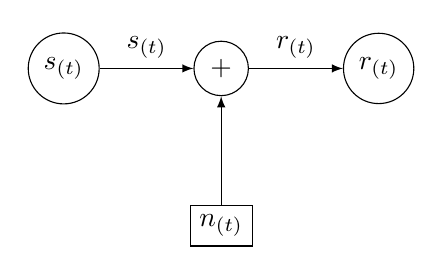
\begin{tikzpicture}[
                        node distance=2cm,
                        >=latex
                    ]
                    % Blocks
                    \node [circle,draw] (TXant) {$s_{(t)}$};
                    \node [circle, draw,right of=TXant] (sum) {$+$};
                    \node [rectangle, draw,below of = sum,minimum height=1em, minimum width=2em] (error) {$n_{(t)}$};
                    \node [circle,draw,right of=sum] (RXant) {$r_{(t)}$};
                
                    % Connections
                    \draw [->] (TXant) --node[above]{$s_{(t)}$} (sum);
                    \draw [->] (sum) --node[above]{$r_{(t)}$} (RXant);
                    \draw [->] (error) -- (sum);
                \end{tikzpicture}    
            \label{fig:Sistema di comunicazione canale con errore}
            \caption{Esempio sistema di canale con errore}
        \end{figure}
        Durante la trasmissione di $s_{(t)}$ viene introdotto dell'errore $n_{(t)}$. $n_{(t)}$ é un segnale completamente aleatorio di varia 
        natura:
        \begin{itemize}
            \item {Termico}
            \item {Interferenze}
            \item {Fading}
            \item {\dots}
        \end{itemize}
        \noindent di conseguenza $r_{(t)} = s_{(t)}+e_{(t)}$ diventa un segnale aleatorio.

        I segnali che analizzo sono tutte quantitá aleatorie: ho bisogno della probabilitá per analizzare la tipologia di segnali, anche per la sorgente
        potrei averne bisogno se non sono nel caso di segnali deterministici.

        \subsubsection{Tipi di modelli matematici}
            Esistono vari tipi di modelli matematici:
            \begin{itemize}
                \item {Deterministico: se esiste certezza e ne possiamo calcolare il valore a ogni istante del tempo (Es. sistemi lineari tempo invarianti)}
                \item {Probabilistico (Aleatorio): se non conosciamo la certezza con cui l'evento puó verificaris ma ne possiamo dare una valutazione probabilistica.}
            \end{itemize}
            Introduciam oquind i
    \subsection{Algebra dei Set (insiemi)}
        Un set é una collezione di elementi che condividono un criterio oggettivo per decidere se appartengono al set o no. Prendiamo come set $A$ e come 
        elemento del set $A$ $x$:
        \begin{itemize}
            \item {Se l'elemento appartiene al set: $x\in A$, veceversa se non appartiene:$x\notin A$}
            \item {Se un set é vuoto: $A=\{\emptyset\}=\emptyset$}
            \item {Se $x_1, \dots, x_n$ sono elementi di $A$ allora:
                \[
                    A=\{x_1, \dots, x_n \}
                \]
            }
        \end{itemize}
        \subsubsection{Operazioni booleane su set}
            \begin{itemize}
                \item {Unione ($A\cup B$): l'unione di due set $A$ e $B$ é a sua volta un set composto dagli elementi che appartegono a $A$ o $B$, o entrambi.}
                \item {Intersezione ($A\cap B$): l'intersezione di due set $A$ e $B$ é a sua volta un set composto dagli elementi che appartegono a $A$ e $B$.
                \begin{figure}[H]
                    \centering
                    \includegraphics[width = 5cm]{media/Unione_Intersezione.png}
                    \caption{Unione e Intersezione} 
                \end{figure}
                }
                \item {Disgiunzione: é una relazione tra due set $A$ e $B$, essi sono disgiunti se tra loro non hanno elementi comuni ($A\cap B = \emptyset $).}
                \item {Partizione ($A = A_1\cup A_2\cup A_3$): la partizione di un insieme $A$ é una divisione dell'insieme stesso in subset disgiunti.
                \begin{figure}[H]
                    \centering
                    \includegraphics[width = 5cm]{media/Insiemi_distinti.png}
                    \caption{Disgiunzione e Partizione} 
                \end{figure}
                }
                \item {Complemento ($A^c$): dati due set $A$ e $B:A\subset B$ il complemento del set $A$ é il set contenente gli elementi di $B$ non appartenenti ad $A$.
                \begin{figure}[H]
                    \centering
                    \includegraphics[width = 5cm]{media/Insieme_Complementare.png}
                    \caption{Complemento}
                \end{figure}
                }
            \end{itemize}
        \subsubsection{Operazioni algebriche su set}
            \begin{itemize}
                \item {Idempotenza
                    \[
                        \left(A^c\right)^c = A
                    \]
                }
                \item {Propietá commutativa
                    \begin{gather}
                        A\cup B = B\cup A \nonumber \\
                        A\cap B = B\cap A \nonumber
                    \end{gather}
                }
                \item {Propietá associativa
                    \begin{gather}
                        (A\cup B) \cup C= (A\cup C)\cup B \nonumber \\
                        (A\cap B) \cap C= (A\cap C)\cap B \nonumber                        
                    \end{gather}
                }
                \item {Propietá distributiva
                    \begin{gather}
                        (A\cup B) \cap C= (A\cap C)\cup (B \cap C) \nonumber \\
                        (A\cap B) \cup C= (A\cup C)\cap (B \cup C) \nonumber                        
                    \end{gather}
                }
            \end{itemize}

    \subsection{Modelli probabilistici}
        La descrizione di un esperimento con risultati incerti é chiamato \emph{modello probabilistico}, la costruzione del modello richiede:
        \begin{itemize}
            \item {Spazio dei campioni o set universale $S$: nel quale sono presenti tutti i possibili risultati dell'esperimento.}
            \item {Una classe di eventi $A$ che sia un subset di $S$.}
            \item {Legge della Probabilitá: alla quale una quantitá non negativa $P[A]$ viene assegnata ad $A$. $P[A]$ viene detta probabilitá dell'evento $A$: rappresenta
                con quale occorrenza potrebbe verificarsi il risultato delĺ'esperimento $A$.}
        \end{itemize}
        \begin{figure}[H]
            \centering
            \includegraphics[width = 5cm]{media/Insieme_probabilita.png}
            \caption{Modello Probabilistico} 
        \end{figure}
        Un evento puó avere come risultato un singolo risultato o un subset di risultati di $S$.
        \subsubsection{Assiomi della probabilitá}
            \begin{enumerate}
                \item \label{Ass. Prob. 1}{Non Negativitá: la probabilitá di $A$ é un numero non negativo:
                    \[
                        0\leq P[A] \leq 1,\ \forall \text{ evento A}
                    \]
                }
                \item \label{Ass. Prob. 2}{Additivitá: se $A$ e $B$ sono due eventi disgiunti, allora la probablitá dell'unione é: 
                    \[
                        P[A\cup B] = P[A] + P[B] 
                    \]
                }
                \item \label{Ass. Prob. 3}{Normalizzazione: la probabilitá del set universale $S$ é $P[S] = 1$}
            \end{enumerate}
            Si sviluppano alcune propietá della probabilitá:
            \begin{itemize}
                \item {
                    La probabilitá di un evento impossibile é zero.
                    Dimostrazione:
                }
                \item {
                    $P[A^c] = 1-P[A]$
                    Dimostrazione:
                }
                \item {
                    Se un evento $A$ é un subset di un evento $B$ allora: $P[A]\leq P[B]$. 
                    Dimostrazione: 
                }
                \item {
                    \begin{sloppypar}
                        Se due eventi $A$ e $B$ non sono disgiunti allora: ${P[A \cup B]= P[A] + P[B] -  P[A\cap B]}$\\
                        Dimostrazione:
                    \end{sloppypar}
                }
            \end{itemize}
        \subsubsection{Probabilitá condizionata}\label{Probabilitá condizionata}
            Prendiamo in esempio un esperimento che implica due eventi $A$ e $B$: $P[A|B]$ sia la probabilitá che un evento $A$ si verifichi
            dato il verificarsi dell'evento $B$, $P[A|B]$ é detta probabilitá condizionata di $A$ dato $B$, assumendo $P[B]\neq 0$:
            \[
                P[A|B] = \frac{P[A\cap B]}{P[B]}
            \]

        \subsubsection{Regola di Bayes}\label{Regola di Bayes}
            Supponiamo che si possano ricavare facilmente le probabilitá $P[A|B]$, $P[A]$ e $P[B]$ e vogliamo trovare la probabilitá condizionata $P[B|A]$:
            \[
                P[B|A] = \frac{P[A|B]P[B]}{P[A]}   
            \]
        \subsubsection{Indipendenza}\label{Indipendenza}
            Supponiamo che l'occorrenza  di un evento $A$ non fornisca nessuna informazione sull'evento $B$, $P[B|A] = 0$. Dalla regola di Bayes abbiamo $P[A|B] = P[A]$,
            i due eventi sono indipendenti e occorre che:
            \[
                P[A\cap B] = P[A]P[B]    
            \]
        \subsubsection{Legge della probabilitá totale}\label{Legge della probabilitá totale}
            Supponiamo $\{ A_n = 1,\dots N\}$ é un insieme di eventi disgiunti:

            \begin{figure}[H]
                \centering
                \includegraphics[width = 5cm]{media/probabilita_totale.png}
            \end{figure}
            \[
                P[B] = \sum_{n=1}^{N}P[B\cap A_n]    
            \]
        \subsubsection{Problemi esempio:}
            \paragraph{Radar Detection Problem:} Nel problema del rilevamento vogliamo analizzare in particolere tre tipi di probabilitá:
                \begin{itemize}
                    \item {
                        \emph{Probabilitá a priori} $P[A]$: probabilitá che il bersaglio sia nell'area.
                    }
                    \item {
                        \emph{Probabilitá di rivelazione} $P[B|A]$: probabilitá che il radar riveli il bersaglio, quando effettivamente il bersaglio
                         é presente nell'area.
                    }
                    \item {
                        \emph{Probabilitá di falso allarme} $P[B|A^c]$: probabilitá che il radar riveli il bersaglio, ma il bersaglio non
                         é effettivamente presente nell'area. 
                    }
                \end{itemize}
                Dati i dati delle relative probabilitá:
                \begin{gather}
                    P[A] = 0.02 \nonumber \\
                    P[B|A] = 0.99 \nonumber \\
                    P[B|A^c] = 0.01 \nonumber 
                \end{gather}
                $A^c$ indica che il bersagli non é presente. Il problema richiede di calcolare la probabilitá condizionata
                $P[A|B]$, la quale definisce la probabilitá che il bersaglio sia presente nell'area e il radar l'abbia rivelata.
                Soluzione:
                \[
                    \overset{\ref{Regola di Bayes}}{\Rightarrow} P[A|B] = \frac{P[A]P[B|A]}{P[B]}    
                \]                    
                Devo solo calcolare $P[B]$:
                \begin{align}
                        \overset{\ref{Legge della probabilitá totale}}{\Rightarrow} P[B] &= \sum_{n=1}^{2} P[B\cap A_n] = \sum_{n=1}^{2} P[B|A_n] P[A_n] \nonumber \\
                        P[B] &= P[B|A]P[A] + P[B|A^c]P[A^c] \nonumber \\
                             &= 0.99\dotproduct 0.02 + 0.01 \dotproduct 0.098 = 0.0296 \cong 0.03  \nonumber       
                \end{align}

                Ricordiamo che $P[A^c] = 1-P[A]$, nel nostro caso il problema ri risolve facilmente applicando il Th della probabilitá totale su due set disgiunti 
                $A$ e $A^c$. Possiamo quindi calcolare la probabilitá condizionata:
                \[
                    P[A|B] = \frac{P[A]P[B|A]}{P[B]} = \frac{0.02 \dotproduct 0.99}{0.03} = 0.66    
                \]

            \paragraph{Communication Problem:} In un sistema di comunicazione ho:
                \begin{itemize}
                    \item {$1$ é trasmesso con probabilitá $P[1] = 0.3$ e $0$ con probabilitá $P[0] = 1-P[1] = 0.7$}
                    \item {la probabilitá di errore é $P_e = 0.01$}
                \end{itemize}
                Richiesta: assumendo che venga ricevuto $0$, calcolare la probabilitá che questo sia stato effettivamente trasmesso.
                Soluzione: Definiamo i set di interesse:
                \begin{itemize}
                    \item {$A = \{0\text{ é stato trasmesso}\},\ A^c = \{1 \text{ é stato trasmesso}\}$}
                    \item {$B = \{0\text{ é stato ricevuto}\},\ B^c = \{1 \text{ é stato ricevuto}\}$}
                \end{itemize}
                \[
                    \overset{\ref{Regola di Bayes}}{\Rightarrow} P[A|B] = \frac{P[A]P[B|A]}{P[B]}    
                \]                           
                $P[B|A]$ non é altro che il probabilitá di corretta ricezione ($P[c]$), posso calcolarla dalla probabilitá di errore:
                \begin{gather}
                    P[e] = P[B^c|A] = P[B|A^c] = 0.01, \text{ probabilitá di errore} \nonumber \\
                    P[c] = P[B|A] = P[B^c|A^c] = 1-P[e]= 0.99, \text{ probabilitá di corretta ricezione}\nonumber 
                \end{gather}
                Calcoliamo $P[B]$:
                \begin{align}
                    \overset{\ref{Legge della probabilitá totale}}{\Rightarrow} P[B] &= \sum_{n=1}^{2} P[B\cap A_n] = \sum_{n=1}^{2} P[B|A_n] P[A_n] \nonumber \\
                    P[B] &= P[B|A]P[A] + P[B|A^c]P[A^c] \nonumber \\
                         &= 0.99\dotproduct 0.7 + 0.01 \dotproduct 0.3 = 0.696 \nonumber       
                \end{align}
                Possiamo quindi calcolare la probabilitá condizionata:
                \[
                    P[A|B] = \frac{P[A]P[B|A]}{P[B]} = \frac{0.7 \dotproduct 0.99}{0.696} = 0.995    
                \]
            \paragraph{Esempio palline:}
                Eventi: Pesco una pallina dall'urna \emph{pippo} e la metto nell'urna \emph{pluto}, infine pesco una pallina dall'urna \emph{pluto}.
                Calcolare la probabilitá di pescare una pallina bianca dall'urna \emph{pluto} ($P[\text{pesco 1 bianca da \emph{pluto}}] = P[A]$).  
                \begin{figure}[H]
                    \centering
                    \includegraphics[width = 4cm]{media/uwu.png}
                \end{figure}
                Definiamo per prima cosa i set del problema:
                \begin{itemize}
                    \item {$A = \{ pesco una pallina bianca da pluto\}$}
                    \item {$B = \{ pesco una pallina bianca da pippo\}$}
                    \item {$B^c = C = \{ pesco una pallina nera da pippo\}$}
                \end{itemize}
                Calcoliamo $P[A]$:
                \begin{align}
                    \overset{\ref{Legge della probabilitá totale}}{\Rightarrow} P[A] &= \sum_{n=1}^{2} P[A\cap B_n] = \sum_{n=1}^{2} P[A|B_n] P[B_n] \nonumber \\
                    P[A] &= P[A|B]P[B] + P[A|C]P[C] \nonumber \\
                         &= \frac{3}{4}\frac{2}{3} + \frac{2}{4}\frac{1}{3} = \frac{2}{3}  \nonumber       
                \end{align}
                \begin{itemize}
                    \item {$P[A|B]$: pesco bianco da \emph{pluto} avendo inserito una bianca da \emph{pippo}}
                    \item {$P[A|C]$: pesco bianco da \emph{pluto} avendo inserito una nera da \emph{pippo}}
                \end{itemize}

                \subparagraph{Aggiungiamo due palline da \emph{pippo} in \emph{pluto}:} Cambia il Th della probabilitá totale:
                    \begin{itemize}
                        \item {$P[B]$: pesco due bianche da \emph{pippo} $= \frac{2}{3}\dotproduct \frac{1}{2} $}
                        \item {$P[A|B]$: pesco due bianche da \emph{pluto} avendo inserito due bianche da \emph{pippo}$= \frac{4}{5} $}
                        \item {$P[C]$: pesco una bianca e una nera da \emph{pippo} $= \frac{2}{3}\dotproduct \frac{1}{2} $}
                        \item {$P[A|C]$: pesco bianco da \emph{pluto} avendo inserito una bianca e una nera da \emph{pippo} $= \frac{3}{5} $}
                        \item {$P[D]$: pesco due nere da \emph{pippo}, é un evento impossibile $P[D] = 0$}
                        \item {$P[A|D]$: pesco bianco da \emph{pluto} avendo inserito due nere da \emph{pippo} $P[D] = 0$}
                        \item {$P[E]$: una nera e una bianca da \emph{pippo}$= \frac{1}{3}\dotproduct 1 $}
                        \item {$P[A|E]$: pesco bianco da \emph{pluto} avendo inserito una nera e una bianca da \emph{pippo} $= \frac{3}{5} $}
                    \end{itemize}
                    \begin{align}
                        \overset{\ref{Legge della probabilitá totale}}{\Rightarrow} P[A] &= \sum_{n=1}^{4} P[A\cap B_n] = \sum_{n=1}^{4} P[A|B_n] P[B_n] \nonumber \\
                        P[A] &= P[A|B]P[B] + P[A|C]P[C]+ P[A|D]P[D]+ P[A|E]P[E] \nonumber \\
                        &= \frac{4}{5}\frac{1}{3} + \frac{3}{5}\frac{1}{3} + 0 + \frac{3}{5}\frac{1}{3} = \frac{10}{15}  \nonumber       
                    \end{align}
        \subsubsection{Coefficiente binomiale}\label{Coefficiente binomiale}
            Il coefficiente binomiale $\binom{n}{k}$ é un numero intero non negativo che fornisce le combiazioni semplici di $n$ elementi di classe $k$,
            definito da:
            \[
                \binom{n}{k} = C(n;k) = \frac{n!}{k!\dotproduct n-k!}
            \]
            Possiamo usarli per calcolare la probabilitá di errore su eventi ripetuti inunione con la distribuzione di bernulli \ref{Probabilita di errore BSC}.
            \paragraph{Esempio su sistema di comunicazione binario:}
                Prendiamo in esempio un trasmettitore di codice binario a ripetizione con $R = \frac{1}{3}
                \begin{cases}
                    0 = [000]\nonumber \\
                    1 = [111]\nonumber    
                \end{cases}$. Calcolare la probabilitá di errore del sistema, $P[E]$, sapendo che la probabilitá di errore sul
                bit é $P[e] = 0.01$.
                Soluzione:
                Scelgo la mia regola di decisione per la decodifica dei bit, a maggioranza:
                \begin{gather}
                    1 \rightarrow \text{Se ho la maggioranza di uno nel codice, nel nostro caso 2 su 3} \nonumber \\
                    0 \rightarrow \text{Se ho la maggioranza di zero nel codice, nel nostro caso 2 su 3} \nonumber
                \end{gather}
                sbaglio il codice in trasmissione se ho sbagliato tre o due bit. Calcoliamo la probabilitá del canale,
                $P[E] \overset{\ref{Legge della probabilitá totale}}{=} P[E|0]P[0] + P[E|1]P[1]$:
                \begin{itemize}
                    \item {$P[E|0]$: Osserviamo tutti i casi possibili di trasmissione del codice di $0 = [000]$
                        \begin{table}[H]
                            \centering
                            \begin{tabular}{cc}
                            Messaggio & Errore \\
                            {[}000{]} &    \\
                            {[}001{]} &    \\
                            {[}010{]} &    \\
                            {[}011{]} &    $E_1$\\
                            {[}100{]} &    \\
                            {[}101{]} &    $E_2$\\
                            {[}110{]} &    $E_3$\\
                            {[}111{]} &    $E_4$
                            \end{tabular}
                        \end{table}
                        Applichiamo la legge della probabilitá totale (\ref{Legge della probabilitá totale}):
                        \[
                            P[E|0] = \sum_{n=1}^{4}P[E_n|0] = P[E_1|0] +P[E_2|0]+P[E_3|0]+P[E_4|0] 
                        \]
                        \begin{itemize}
                            \item {$P[E_1|0] = P[E_2|0] = P[E_3|0] = P[e]P[e]P[c]$,$P[c] = 1-P[e]$ corretta trasmissione, sono uguali poiché non ci interessa l'ordine con cui appare l'errore}
                            \item {$P[E_4|0] = P[e]P[e]P[e]$}
                        \end{itemize}
                        \begin{align}
                            P[E|0] &= 3P^2[e](1-P[e])+ P^3[e] = 3P^2[e]-3P^3[e]+P[e] \nonumber \\
                                   &= 3P^2[e] -2P^3[e] \cong 3P^2[e]\nonumber
                        \end{align}
                    }
                    \item {$P[E|1]$: Usiamo la probabilitá di erore sul canale \ref{Probabilita di errore BSC}
                        \[
                            P[E|1] = \binom{3}{3}P^3[e] +\binom{3}{2}P^2[e] (1-P[e]) \cong 3 P^2[e]
                        \]
                    }
                \end{itemize}         
                Abbiamo quindi:
                \[
                    P[E] =P[E|0]P[0] + P[E|1]P[1] = 3 P^2[e] P[0]+3 P^2[e]P[1] \cong 3 P^2[e]
                \] 
                \subparagraph{Caso $R=\frac{1}{5}$:}
                    \begin{align}
                        P[E] &= \sum_{n=3}^{5}\binom{5}{n}P^n[e](1-P[e])^{5-n} \nonumber \\
                             &= \binom{5}{3}P^3[e](1-P[e])^{2}+\binom{5}{4}P^4[e](1-P[e])^{1}+\binom{5}{5}P^5[e](1-P[e])^{0}\nonumber
                    \end{align}
            \paragraph{Esempio prove ripetute:} Abbiamo 2 monete, una regolare ($r$) e una truccata ($t$) con le seguenti probabilitá:
            \[
                \begin{cases}
                    P_r[T] = \frac{1}{2}\nonumber \\
                    P_r[C] = \frac{1}{2}\nonumber
                \end{cases},
                \begin{cases}
                    P_t[T] = \frac{8}{10}\nonumber \\
                    P_t[C] = \frac{2}{10}\nonumber
                \end{cases}
            \]
            Calcolare la probabilitá di aver scelto la moneta regolare se: scelgo a caso una monetina tra le due e la lancio $10$ volte
            osservando che esce 5 volte croce e 5 volte testa.
            Soluzione: la probabilitá da calcolare é 
            \[
                P[A|B] = ? \Rightarrow \begin{cases}
                    A = \text{ho scelto la moneta regolare}\nonumber \\
                    A^c = C = \text{scelgo la moneta truccata}\nonumber \\
                    B = \text{ esce 5 volte testa e 5 volte croce}\nonumber
                \end{cases}  
            \]
            \[
                \overset{\ref{Regola di Bayes}}{\Rightarrow} P[A|B] = \frac{P[A]P[B|A]}{P[B]},\ P[B|A] = ?\ e\ P[B] = ?\nonumber \\
            \]
            \begin{align}
                P[B] &\overset{\ref{Legge della probabilitá totale}}{ = } P[B|A]P[A] + P[B|C]P[C] \nonumber \\
                P[B|A] & = \binom{10}{5} P_r[T]^5P_r[C]^5 = \binom{10}{5} \left(\frac{1}{2}\right)^{10}\nonumber \\
                P[B|C] & = \binom{10}{5} P_r[T]^5P_r[C]^5 = \binom{10}{5} \left(\frac{8}{10}\right)^5\left(\frac{2}{10}\right)^5\nonumber
            \end{align}
            inserendo dentro bayes il risultato dovrebeb essere $0.9$.
    \subsection{Variabili Aleatorie - Random Variables}
        Una \emph{variabile aleatoria} $X$ é una funzione il cui dominio é un insieme, di numeri reali, dello spazio degli esiti di un esperimento. ogni spazio degli esiti
        ha la sua probabilitá associata. 
        \begin{figure}[H]
            \centering
            \includegraphics[width = 5cm]{media/insieme variabili aleatorie.png}
            \caption{Esperimento $\rightarrow$ Intervallo $\rightarrow$ Probabilitá dell'Intervallo}
        \end{figure}
        Una variabile aleatoria puó essere continua o discreta. Le variabil ialeatorie si indicano con le lettere
        maiuscole
        \subsubsection{Funzioni di Distribuzione - Distribution Functions}
            Considera la variabile aleatoria $X$ e la probabilitá dell'evento $X\leq x$, per convenzione si indica con $P[X\leq x]$,
            che puó essere scritto come:
            \[
                F_{X(x)} \triangleq P[X\leq x]\ \forall x    
            \]
            La funzione $F_{X(x)}$ é chiamata la \emph{funzione distribuzione} della variabile $X$, si puó notare che é funizone di $x$ non di 
            $X$.
            \paragraph{Propietá:}
                \begin{itemize}
                    \item {Limitata - Boundeness: é limitata tra zero e uno, essendo una probabilitá.}
                    \item {Monotona - Monotonicity: la funzione é una funzione monotona \emph{non decrescente} (puó rimanere costante) di $x$.}
                \end{itemize}
        \subsubsection{Funzione Densitá di Probabilitá - Probability Density Function (pdf)}
            La variabile aleatoria $X$ é continua se la funzione distribuzione $F_{X(x)}$ é differenziabile:
            \[
                f_{X(x)} = \derivative{}{x}F_{X(x)}\ \forall x    
            \]
            $f_{X(x)}$ é detta \emph{funzione di densitá di probabilitá} (pdf).
            \paragraph{Propietá:}
                \begin{itemize}
                    \item {Non negativa}
                    \item {Normalization: l'area totale della $pdf$ é unitaria.}
                    \item {
                        \begin{align}
                            P[x_1<X<x_2] &= P[X\leq x_2]  - P[X\leq x_1] = F_{X(x_2)} - F_{X(x_1)}  \nonumber \\
                                         &= \int_{x_1}^{x_2} f_{X(x)} dx\nonumber
                        \end{align}
                        se non avessi un estremo:
                        \begin{itemize}
                            \item {$ P[X\leq x_2] = \int_{-\infty}^{x_2}$}
                            \item {$ P[X\leq x_1] = 1-\int_{-\infty}^{x_1}$}
                        \end{itemize}
                    }
                \end{itemize}
            \paragraph{Esempio - Distribuzione Uniforme:} 
                Proviamo le propietá della funzione distribuzione $F_{X(x)}$ e la funzione densitá di probabilitá $f_{X(x)}$ per una variabile aleatoria
                continua:
                \[
                    f_{X(x)} = 
                    \begin{cases}
                        0 & x\leq a\nonumber \\
                        \frac{1}{b-a} & a<x\leq b\nonumber \\
                        0 & x>b\nonumber
                    \end{cases}  
                \]
                Integrandola troviamo:
                \[
                    F_{X(x)} = 
                    \begin{cases}
                        0 & x\leq a\nonumber \\
                        \frac{x-a}{b-a} & a<x\leq b\nonumber \\
                        1 & x>b\nonumber
                    \end{cases}  
                \]
                \begin{figure}[H]
                    \centering
                    \subfloat[$f_{X(x)}$]{
                        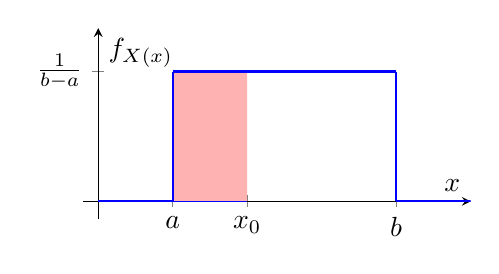
\begin{tikzpicture}
                            \begin{axis}[
                                xlabel=$x$,
                                ylabel=$f_{X(x)}$,
                                xmin=-0.2,
                                xmax=5,
                                ymin=-0.2,
                                ymax=2,
                                ytick = {1.5},
                                xtick={0, 1,2, 4},
                                xticklabels={$0$, $a$,$x_0$, $b$},
                                yticklabels = {$\frac{1}{b-a}$},
                                %yticklabel style = {yshift=5pt,xshift=4pt}, 
                                axis lines=middle,
                                thick,
                                domain=-4:4,
                                samples=100,
                                width=6.5cm,
                                height=4cm
                            ]
                        
                            \addplot [const plot, blue, thick] coordinates{(1,1.5)(4,1.5)};
                            \addplot [const plot, blue, thick] coordinates{(1,0)(1,1.5)};
                            \addplot [const plot, blue, thick] coordinates{(4,0)(4,1.5)};
                            \addplot [const plot, blue, thick] coordinates{(4,0)(5,0)};
                            \addplot [const plot, blue, thick] coordinates{(0,0)(1,0)};
                        
                            \addplot [const plot, blue, thin, name path = A] coordinates{(1,1.5)(2,1.5)};
                            \addplot [const plot, blue, thin, name path = B] coordinates{(1,0)(2,0)};
                        
                        
                            \addplot[red,opacity = 0.3] fill between[of=A and B];
                        


                            \end{axis}
                        \end{tikzpicture}
                    }
                    \hfill
                    \subfloat[$F_{X(x)}$]{
                        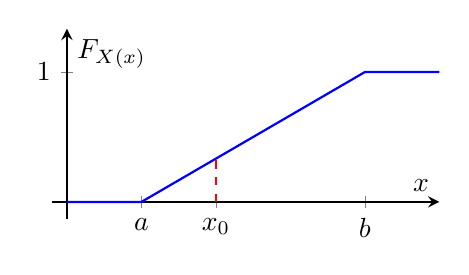
\begin{tikzpicture}
                            \begin{axis}[
                                xlabel=$x$,
                                ylabel=$F_{X(x)}$,
                                xmin=-0.2,
                                xmax=5,
                                ymin=-0.2,
                                ymax=2,
                                ytick = {1.5},
                                xtick={0, 1, 2,4},
                                xticklabels={$0$, $a$, $x_0$, $b$},
                                yticklabels = {$1$},
                                %yticklabel style = {yshift=5pt,xshift=4pt}, 
                                axis lines=middle,
                                thick,
                                domain=-5:5,
                                samples=100,
                                width=6.5cm,
                                height=4cm
                            ]
        
                            \addplot [sharp plot, blue, thick] coordinates{(0,0)(1,0)(4,1.5)(5,1.5)};
                            \addplot [dashed, red, thick] coordinates{(2,0)(2,0.5)};
        
                            \end{axis}
                        \end{tikzpicture}
                    }
                    \caption{Distribuzione Uniforme}
                    \label{Distribuzione Uniforme}
                \end{figure}
        \subsubsection{Funzione Probabilitá di massa - Probability Mass Function (pmf)}
            Consideriamo il caso di una variabile aleatoria discreta $X$, la quale puó assumere un numero rinito o infinito di valori. La funzione 
            distribuzione $F_{X(x)}$ si applica anche alle variabili discrete, ma non é differenziabile per come l'abbiamo definita. Definiamo 
            la funzione probabilitá di massa $p_{X(x)}$:
            \[
                p_{X(x)} \triangleq P[X = x]    
            \]
            é la probabilitá di un evento $X=x$, che consiste in tutti i possibili risultati di un esperimento i quali hanno un valore di 
            $X$ uguale a $x$.

            \paragraph{Esempio di Bernulli}
                Consideriamo l'esperimento probabilistico che assume uno di due valori:
                \begin{itemize}
                    \item {il valore 1 con probabilitá $p$}
                    \item {il valore 0 con probabilitá $1-p$}
                \end{itemize}
                Tale variabile aleatoria é chiamata \emph{variabile aleatoria di Bernulli}:
                \begin{figure}[H]
                    \centering
                    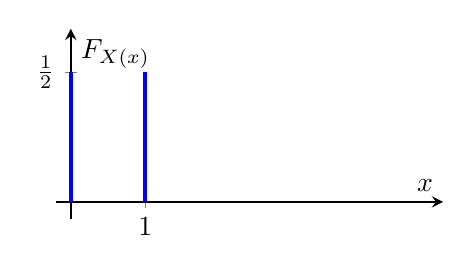
\begin{tikzpicture}
                        \begin{axis}[
                            xlabel=$x$,
                            ylabel=$F_{X(x)}$,
                            xmin=-0.2,
                            xmax=5,
                            ymin=-0.2,
                            ymax=2,
                            ytick = {1.5},
                            xtick={0, 1},
                            xticklabels={$0$, $1$},
                            yticklabels = {$\frac{1}{2}$},
                            %yticklabel style = {yshift=5pt,xshift=4pt}, 
                            axis lines=middle,
                            thick,
                            domain=-5:5,
                            samples=100,
                            width=6.5cm,
                            height=4cm
                        ]
    
                        \addplot [const plot, blue,ultra thick] coordinates{(0,0)(0,1.5)};
                        \addplot [const plot, blue,ultra thick] coordinates{(1,0)(1,1.5)};
    
                        \end{axis}
                    \end{tikzpicture}
                \end{figure}
        \subsubsection{ - Multiple Random Variables}
            Consideriamo due variabili aleatorie $X$ e $Y$:
            \begin{itemize}
                \item {
                    La funzione distribuzione $F_{X,Y (x,y)}$ é la probabilitá che $X$ sia minore o uguae a un valore specifico $x$ e che $Y$
                    sia minore o uguale a un'altro valore specifico $y$:
                    \[
                        F_{X,Y (x,y)} = P[X\leq x,Y\leq y]    
                    \]
                }
                \item {
                    La funzione densitá di probabilitá $f_{X,Y (x,y)}$ contiene tutto quello che ci serve per fare una completa analisi della probabilitá
                    di piú variabili aleatorie:
                    \[
                        f_{X,Y (x,y)} = \frac{d^2 F_{X,Y (x,y)}}{dxdy}     
                    \]

                }
            \end{itemize}
        \subsubsection{Funzione Densitá di Probabilitá Condizionata - Conditional Probability Density Function}
            Supponendo che $X$ e $Y$ siano due variabili aleatorie continue con $f_{X,Y (x,y)}$, la funzione densitá di probabilitá condizionata di $Y$ con $X=x$,
            é definita da:
            \[
                f_{Y (y|x)} = \frac{f_{X,Y (x,y)}}{f_{X(x)}}     
            \]
            Supponendo che le due variabili siano indipendenti: allora $f_{Y (y|x)}$ si riduce alla densitá marginale $f_{Y (y)}$ e la funzione densitá di
            probabilitá diventa $f_{X (x)}f_{Y (y)}$, se cosí fosse le due variabili si dicono \emph{statisticamente indipendenti}\index{Statisticamente Indipendenti}.
        \subsubsection{Somma di Variabili Aleatorie Indipendenti}
            Consideriamo due variabili aleatorie $X$ e $Y$ statisticamente indipendenti e continue con funzioni di densitá di probabilitá $f_{X (x)}$ e $f_{Y (y)}$ si 
            definisce $Z = X+Y$ la cui $pdf$ $f_{Z (z)}$ é:
            \[
                f_{Z (z)} = \int_{-\infty}^{\infty}f_{X (x)}f_{Y (z-y)} dx =  f_{X (x)} \otimes f_{Y (y)}
            \]
            La somma di due variabili aleatoria indipendeti e continue é la convoluzione delle funzioni di densitá di probabilitá.    
            Dimostrazione: (To DO: sul libro)
            \begin{figure}[H]
                \centering
                \subfloat[$f_{X(x)}$]{
                    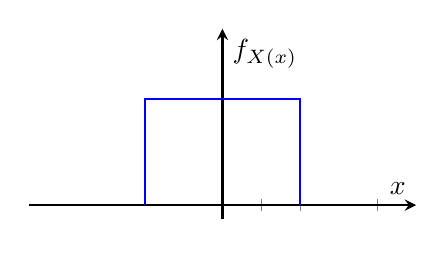
\begin{tikzpicture}
                        \begin{axis}[
                            xlabel=$x$,
                            ylabel=$f_{X(x)}$,
                            xmin=-5,
                            xmax=5,
                            ymin=-0.2,
                            ymax=2.5,
                            ytick = {1.5},
                            xtick={0, 1,2, 4},
                            xticklabels={},
                            yticklabels = {},
                            %yticklabel style = {yshift=5pt,xshift=4pt}, 
                            axis lines=middle,
                            thick,
                            domain=-5:5,
                            samples=100,
                            width=6.5cm,
                            height=4cm
                        ]
                        \addplot [const plot, blue, thick] coordinates{(-2,0)(-2,1.5)(2,1.5)(2,0)};
                        \end{axis}
                    \end{tikzpicture}
                }
                \hfill
                \subfloat[$f_{Y(y)}$]{
                    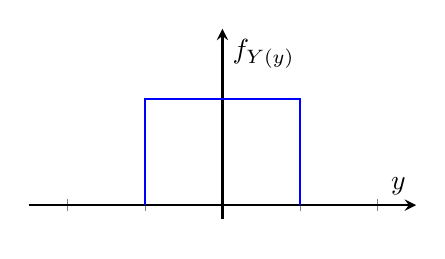
\begin{tikzpicture}
                        \begin{axis}[
                            xlabel=$y$,
                            ylabel=$f_{Y(y)}$,
                            xmin=-5,
                            xmax=5,
                            ymin=-0.2,
                            ymax=2.5,
                            ytick = {1.5},
                            xtick={},
                            xticklabels={},
                            yticklabels = {},
                            %yticklabel style = {yshift=5pt,xshift=4pt}, 
                            axis lines=middle,
                            thick,
                            domain=-5:5,
                            samples=100,
                            width=6.5cm,
                            height=4cm
                        ]
    
                        \addplot [const plot, blue, thick] coordinates{(-2,0)(-2,1.5)(2,1.5)(2,0)};
                        \end{axis}
                    \end{tikzpicture}
                }

                \subfloat[$f_{Z(z)}$]{
                    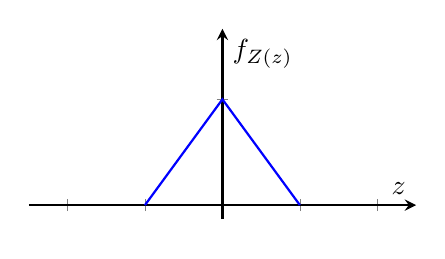
\begin{tikzpicture}
                        \begin{axis}[
                            xlabel=$z$,
                            ylabel=$f_{Z(z)}$,
                            xmin=-5,
                            xmax=5,
                            ymin=-0.2,
                            ymax=2.5,
                            ytick = {1.5},
                            xtick={},
                            xticklabels={},
                            yticklabels = {},
                            %yticklabel style = {yshift=5pt,xshift=4pt}, 
                            axis lines=middle,
                            thick,
                            domain=-5:5,
                            samples=100,
                            width=6.5cm,
                            height=4cm
                        ]
                        \addplot [sharp plot, blue, thick] coordinates{(-2,0)(0,1.5)(2,0)};
                        \end{axis}
                    \end{tikzpicture}
                }
                \caption{Somma di Variabili Aleatorie}
                \label{Somma di Variabili Aleatorie}
            \end{figure}
        \subsubsection{Valore medio delle Variabili Aleatorie - Mean Value of Random Variables (Expectation)}\label{Expectation}\index{Expectation}
            L'expectation o il valore medio di ua variabile aleatoria continua $X$ é formalemnte definito da:
            \begin{itemize}
                \item {Caso Continuo:
                    \[
                        \mu_X = \mathbb{E}[X] = \int_{-\infty}^{\infty} xf_{X(x)}dx
                    \]
                }
                \item {Caso Discreto:
                    \[
                        \mathbb{E}[X] = \sum_{x}xp_{X(x)}
                    \]
                }
            \end{itemize}
            é la media pesata delle variabili aleatorie, puó anche essere un valore che non gli appartiene.
            \paragraph{Propietá}
                \begin{itemize}
                    \item {\label{linearita expectation} Linearitá - Linearity: $\mathbb{E}[Z] = \mathbb{E}[X+Y]  = \mathbb{E}[X] +\mathbb{E}[Y]$.}
                    \item {\label{Indipendenza statistica}Indipendenza Statistica - Statistical Indipendence:$\mathbb{E}[Z] = \mathbb{E}[XY] = \mathbb{E}[X] \mathbb{E}[Y]$ 
                    se $X$ e $Y$ sono statisticamente indipendenti.\\
                    Dimostrazione:
                    \begin{align}
                        \mathbb{E}[XY] &= \int_{-\infty}^{\infty}\int_{-\infty}^{\infty} xy f_{X,Y (x,y)} dxdy \overset{Indipendenza}{=} \int_{-\infty}^{\infty}\int_{-\infty}^{\infty} xy f_{X (x)}f_{Y (y)} dxdy \nonumber \\
                                       &= E[X]E[Y] \nonumber
                    \end{align}
                    }
                    \item {\label{valor medio expectation} Teorema del valore medio dell'expectation: 
                        \[
                            \mathbb{E}[g_{(x)}] \overset{Y=g_{(x)}}{=} \mathbb{E}[Y] =  \int_{-\infty}^{\infty}yf_{Y(y)}dy \triangleq \int_{-\infty}^{\infty}g_{(x)}f_{X(x)}dx
                        \]
                    }
                \end{itemize}
            \paragraph{Esempi:}\label{esempi expectation}
                \begin{enumerate}
                    \item{
                        Calcolare il valore medio ($\mu_X$) di:
                        \begin{figure}[H]
                            \centering
                            \begin{tikzpicture}
                                \begin{axis}[
                                    xlabel=$x$,
                                    ylabel=$f_{X(x)}$,
                                    xmin=-0.2,
                                    xmax=5,
                                    ymin=-0.2,
                                    ymax=2.5,
                                    ytick = {1.5},
                                    xtick={1,3},
                                    xticklabels={$a$,$b$},
                                    yticklabels = {$\frac{1}{b-a}$},
                                    axis lines=middle,
                                    domain=0:5,
                                    samples=100,
                                    width=6.5cm,
                                    height=4cm
                                ]
                                \addplot [const plot, blue, thick] coordinates{(1,0)(1,1.5)(3,1.5)(3,0)};
                                \end{axis}
                            \end{tikzpicture}
                        \end{figure}

                        \begin{align}
                            \mu_X &= \int_{-\infty}^{\infty}xf_{X(x)}dx = \int_{a}^{b}\frac{x}{b-a}dx = \eval{\frac{x^2}{2(b-a)}}_{a}^{b}\nonumber \\
                                  &= \frac{b^2-a^2}{2(b-a)} = \frac{b+a}{2}\nonumber 
                        \end{align}
                    }
                    \item{
                        Calcoliamo il valore quadratico medio della distribuzione unitaria ($\mathbb{E}[x^2]$):
                        \begin{align}
                            \mathbb{E}[X^2] &= \int_{-\infty}^{\infty}x^2f_{X(x)}dx = \int_{a}^{b}\frac{x^2}{b-a}dx = \eval{\frac{x^3}{3(b-a)}}_{a}^{b}\nonumber \\
                                            &= \frac{b^3-a^3}{3(b-a)} = \frac{b^2+ab+a^2}{3}\nonumber 
                        \end{align}
                    }
                \end{enumerate}
        \subsubsection{Varianza - Variance}
            La varianza $\sigma^2_x$ di una variabile aleatoria $X$ é definita:
            \[
                var[X] = \mathbb{E}[(X-\mu_X)^2] = \int_{-\infty}^{\infty} (X-\mu_X)^2f_{X(x)}dx
            \]  
            \begin{align}
                var[X] &= \sigma^2_x \overset{\ref{linearita expectation}}{=} \mathbb{E}[X^2-2\mu_XX+\mu_X^2] = \mathbb{E}[X^2]-2\mu_X\mathbb{E}[X]+\mu_X^2 \nonumber \\
                           &= \mathbb{E}[X^2]-\mu_X^2 \nonumber 
            \end{align}\index{Valore quadratico medio}
            $\mathbb{E}[X] = \int_{-\infty}^{\infty} xf_{X(x)}dx$ mentre $\mathbb{E}[X^2] = \int_{-\infty}^{\infty} x^2f_{X(x)}dx$, l'expectation é il peso che diamo alla funzione $f_{X(x)}$.  
            Misura la "randomicitá" di una variabile aleatoria, meno é randomica piú sono vicino al mio valor medio.
            \[
                P[|X-\mu_X|\geq \mathcal{E}]\leq \frac{\sigma^2_X}{\mathcal{E}^2}
            \]
            \paragraph{Deviazione Standard:} $\sigma_X = \sqrt[2]{\sigma^2_X}$ si dice Deviazione Standard
        \subsubsection{Covarianza - Covariance}
            Siano $X$ e $Y$ due variabili aleatorie, si definisce covarianza:
            \begin{gather}
                cov[XY] = \mathbb{E}[(X-\mathbb{E}[X])(Y-\mathbb{E}[Y])]\nonumber\\
                = \mathbb{E}[XY]-\mu_X\mu_Y\nonumber
            \end{gather}
            Il \emph{coefficiente di correlazione}\index{Coefficiente di Correlazione} di $X$ e $Y$ é:
            \[
                \rho_{(X,Y)} = \frac{cov[XY]}{\sigma_X\sigma_Y}
            \]
            misura la somiglianza tra $X$ e $Y$. Le due variabili si dicono:
            \begin{itemize}
                \item {
                    Incorrelate: se la $cov[XY] =0$, ció non implica l'indipendenza delle variabili.
                }
                \item {
                    Ortogonali: se $\mathbb{E}[XY] = 0$
                }
            \end{itemize}
        \subsubsection{Distribuzione Gaussiana}
            \begin{figure}[H]
                \centering
                    \begin{tikzpicture}
                        \begin{axis}[
                            xlabel=$x$,
                            ylabel=$f_{X(x)}$,
                            xmin=-5,
                            xmax=5,
                            ymin=-0.2,
                            ymax=0.8,
                            xtick={},
                            yticklabel style = {font = \scriptsize}, 
                            xticklabels={},
                            axis lines=middle,
                            domain=-5:5,
                            width=12cm,
                            height=5cm
                        ]
                        \addplot [const plot, blue, thick, samples = 500] {gauss(0,0.7)};
                        \end{axis}
                    \end{tikzpicture}
                \caption{Gaussiana}
            \end{figure}               
            Una variabile aleatoria $X$ é detta Gaussiana se la funzione distribuzione di probabilitá ,$pdf$, ha la forma:
            \[
                f_{X(x)} = \frac{1}{\sqrt{2\pi}\sigma_X}e^{\left[\displaystyle -\frac{(x-\mu_X)^2}{2\sigma^2_X}\right]}  
            \]
            \paragraph{Propietá:}\label{propieta distr gaussiana}
            \begin{itemize}
                \item {Definita unicamente da valore medio di $X$ e la varianza $\mathcal{N}(\mu_X,\sigma_X^2)$.}
                \item {\begin{sloppypar}
                    La propietá di Gaussianitá é preservata dalle trasformazioni lineari. ${X \sim \mathcal{N}(\mu_X,\sigma_X^2): Y = \alpha X+\beta}$, calcoliamo come variano 
                    valor medio e varianza:
                \end{sloppypar}
                    \begin{itemize}
                        \item {Valor medio:
                            \[
                                \mathbb{E}[Y] = \mu_Y = \mathbb{E}[\alpha X+\beta]  \overset{\ref{linearita expectation}}{=} \alpha \mathbb{E}[X] + \beta
                            \]
                        }
                        \item {Varianza:
                            \begin{align}
                                \sigma_Y^2  &= \mathbb{E}[Y^2] -\mathbb{E}[Y]^2 =\mathbb{E}[(\alpha X + \beta)^2] -(\alpha \mathbb{E}[X] + \beta)^2 \nonumber \\
                                            &= \mathbb{E}[\alpha^2 X^2 + \beta^2 +2\alpha\beta X] -(\alpha^2 \mathbb{E}[X]^2 + \beta^2 +2\alpha\beta\mathbb{E}[X])\nonumber \\
                                            &= \alpha^2 \mathbb{E}[X^2] + \beta^2 +2\alpha\beta \mathbb{E}[X] -\alpha^2 \mathbb{E}[X]^2 - \beta^2 -2\alpha\beta\mathbb{E}[X]\nonumber \\
                                            &= \alpha^2 \mathbb{E}[X^2] -\alpha^2 \mathbb{E}[X]^2 = \alpha^2 (\mathbb{E}[X^2] -\mathbb{E}[X]^2)\nonumber \\
                                            &= \alpha^2 (\mathbb{E}[X^2] -\mu_X^2)=\alpha^2 \sigma_X^2\nonumber
                            \end{align}                         
                            la costante $\beta$ non influisce la varianza.  
                        }
                    \end{itemize}}
                \item {La somma $Z = X+Y$ di variabili aleatorie Gaussiane indipendenti é anche essa na variabile aleatoria
                    Gaussiana, con:
                        \begin{itemize}
                            \item {$\mathbb{E}[Z] = \mathbb{E}[X] +\mathbb{E}[Y] $}
                            \item {$var[Z] = var[X] +var[Y] $}
                        \end{itemize}}
            \end{itemize}
            \paragraph{Distribuzione Gaussiana Standard}
                Si dice forma Gaussiana Standard se: $\mathbb{E}[X] = 0$ e $var[X] = 1$, $\mathcal{N}(0,1)$:
                \begin{gather}
                    f_{X(x)} = \frac{1}{\sqrt{2\pi}} e^{\displaystyle\left(-\frac{x^2}{2}\right)}\nonumber \\
                    F_{X(x)} =P[X\leq x] = \int_{-\infty}^{\infty}f_{X(x)} =\frac{1}{\sqrt{2\pi}} \int_{-\infty}^{x}e^{\displaystyle\left(-\frac{t^2}{2}dt\right)}\nonumber 
                \end{gather}

                \begin{figure}[H]
                    \centering
                    \subfloat[$f_{X(x)}$]{
                        \begin{tikzpicture}
                            \begin{axis}[
                                xlabel=$x$,
                                ylabel=$f_{X(x)}$,
                                xmin=-5,
                                xmax=5,
                                ymin=-0.2,
                                ymax=0.8,
                                xtick={},
                                yticklabel style = {font = \scriptsize}, 
                                xticklabels={},
                                axis lines=middle,
                                domain=-5:5,
                                samples=100,
                                width=6.5cm,
                                height=5cm
                            ]
                            \addplot [const plot, blue, thick, samples = 300] {gauss(0,1)};
                            \end{axis}
                        \end{tikzpicture}
                    }
                    \hfill
                    \subfloat[$F_{X(x)}$]{
                        \includegraphics[width = 6cm]{media/funzione distribuzione gaussiana.png}
                    }
                    \caption{Distribuzione Gaussiana Standard}
                \end{figure}
                Osservazioni: la varianza permette di modificare la spanciatura della gaussiana, mentre il valor medio shifta sull'asse x la gaussiana.

                Posso utilizzare la forma standard della gaussiana e le trasformazioni lineari per rappresentare qualsiasi altro tipo di gaussiana:
                \[
                    Y\sim \mathcal{N}(\mu_y,\sigma_Y^2) \rightarrow Y = \sigma_Y X + \mu_y
                \]
                Calcoliamo $\mu_Y$ e $\sigma_Y^2$:
                \begin{itemize}
                    \item {$\mathbb{E}[Y] = \mu_Y$}
                    \item {$\sigma_Y^2 = \sigma_X^2 \sigma_Y^2 $}
                \end{itemize}
        \subsubsection{Funzione $Q_{(x)}$}
            Per calacolare la funzione distribuzione di probabilitá ($F_{X(x)}$) non calcoliamo l'integrale della funzione distribuzione di probabilitá, 
            ma utilizziamo la funzione $Q_{(x)}$ cosí definita:
            \[
                Q_{(x)} = 1-F_{X(x)} = P[X\geq x]  
            \]
            formalmente é cosi definita:
            \[
                Q_{(x)} = 1-F_{X(x)} = 1 - \frac{1}{\sqrt{2\pi}} \int_{-\infty}^{x}e^{\left(-\frac{t^2}{2}dt\right)} = \frac{1}{\sqrt{2\pi}} \int_{x}^{\infty}e^{\left(-\frac{t^2}{2}dt\right)}  
            \]
            é l'area sottesa dalla funzione di distribuzione Gaussiana da $x$ all'infinito

            \begin{figure}[H]
                \centering
                \subfloat[$f_{X(x)}$]{
                    \begin{tikzpicture}
                        \begin{axis}[
                            xlabel=$x$,
                            ylabel=$f_{X(x)}$,
                            xmin=-5,
                            xmax=5,
                            ymin=-0.2,
                            ymax=0.8,
                            xtick={1},
                            yticklabel style = {font = \scriptsize}, 
                            xticklabels={$x$},
                            axis lines=middle,
                            domain=-5:5,
                            samples=100,
                            width=7cm,
                            height=5cm
                        ]
                        \addplot [const plot, blue, thick, samples = 300] {gauss(0,1)};
                        \addplot [const plot, blue,name path = A, thick, samples = 300, domain = 1:5] {gauss(0,1)};
                        \addplot [const plot, black,name path = B, thin] coordinates{(1,0)(5,0)};

                        \addplot[red,opacity = 0.3] fill between[of=A and B];
                        \end{axis}
                    \end{tikzpicture}
                }
                \caption{\color{red}$Q_{(x)}$}
            \end{figure}
            \paragraph{Propietá:}
            \begin{itemize}
                \item {$Q_{(x)} = 1-Q_{(-x)}$

                        \begin{figure}[H]
                            \centering
                                \begin{tikzpicture}
                                    \begin{axis}[
                                        xlabel=$x$,
                                        ylabel=$f_{X(x)}$,
                                        xmin=-5,
                                        xmax=5,
                                        ymin=-0.2,
                                        ymax=0.8,
                                        xtick={-1,1},
                                        yticklabel style = {font = \scriptsize}, 
                                        xticklabels={$-x$,$x$},
                                        axis lines=middle,
                                        domain=-5:5,
                                        samples=100,
                                        width=7cm,
                                        height=5cm
                                    ]
                                    \addplot [const plot, blue, thick, samples = 300] {gauss(0,1)};
                                    \addplot [const plot, blue,name path = A, thick, samples = 300, domain = 1:5] {gauss(0,1)};
                                    \addplot [const plot, black,name path = B, thin] coordinates{(1,0)(5,0)};
                                    \addplot [const plot, blue,name path = C, thick, samples = 300, domain = -5:-1] {gauss(0,1)};
                                    \addplot [const plot, black,name path = D, thin] coordinates{(-5,0)(-1,0)};

                                    \addplot[red,opacity = 0.3] fill between[of=A and B];
                                    \addplot[yellow,opacity = 0.3] fill between[of=C and D];
                                    \end{axis}
                                \end{tikzpicture}
                            
                            \caption{{\color{red}$Q_{(x)}$},{\color{yellow}$1-Q_{(-x)}$}}
                        \end{figure}
                }
                \item {$Q_{(\infty)} = 0$}
                \item {$Q_{(-\infty)} = 1$}
                \item {$Q_{(0)} = \frac{1}{2}$}
            \end{itemize}
            utilizziamo la tavola della funzione $Q$
            \begin{figure}[H]
                \centering
                \includegraphics[width = 8cm]{media/grafo funzione q.png}
                \caption{Grafico $Q_{(x)}$}
            \end{figure}
        \subsubsection{Teorema del Limite Centrale - Central Limit Theorem}\label{Teorema del Limite Centrale - Central Limit Theorem}
            Siano $X_1,\dots,X_n$ una sequenza di variabili aleatorie indipendenti e identicamente distribuite con valore medio $\mu$ e varianza $\sigma$:
            \[
                Y_n = \frac{1}{\sigma\sqrt{n}}\left(\sum_{i=1}^{n}X_i-n\mu\right)    
            \]
            al tendere di $n$ all'infinito, $Y_n$ converge alla variabile aleatoria Gaussiana standard:
            \[
                F_{Y(y)} =P[Y\leq y] = \frac{1}{\sqrt{2\pi}} \int_{-\infty}^{y}e^{\left(-\frac{x^2}{2}dx\right)}    
            \]
        \subsubsection{Calcolo probabilitá di errore di un sistema} 
            Dato un sistema binario di comunicazione ($S\in\{0,1\}$), dopo il campionamento ho: $Y = \sqrt{p}S+n$. $p$ é la potenza e $n$ é il rumore
            gaussiano $n \sim \mathcal{N}(0,\sigma_n^2)$. Voglio calcolarne la probabilitá di errore:
            \[
                P_e \overset{\ref{Legge della probabilitá totale}}{=} P_r(\hat{S}=1|S=-1)P(S=-1)+ P_r(\hat{S}=-1|S=1)P(S=1)   
            \] 
            \begin{sloppypar}
                \noindent analizziamo il caso generico in cui ${P(S=1) = q, P(S=-1)=1-q}$, nel caso equiprobabile sarebbero $\frac{1}{2}$: dobbiamo calcolare 
                ${P_r(\hat{S}=1|S=-1)}$ e ${P_r(\hat{S}=-1|S=1)}$
            \end{sloppypar}
            \begin{itemize}
                \item {$P_r(\hat{S}=1|S=-1)$:
                    \[
                        \eval*{Y}_{S = -1} = -\sqrt{p}+n \sim \mathcal{N}(-\sqrt{p},\sigma_Y = \sigma_n^2)  
                    \]
                    al rumore viene solo aggiunta una costante, quindi rimane tale e con distribuzione:
                    \begin{figure}[H]
                        \centering
                            \begin{tikzpicture}
                                \begin{axis}[
                                    xlabel=$x$,
                                    ylabel=$f_{X(x)}$,
                                    xmin=-10,
                                    xmax=10,
                                    ymin=-0.2,
                                    ymax=0.8,
                                    xtick={-1},
                                    yticklabel style = {font = \scriptsize}, 
                                    xticklabels={$-\sqrt{p}$},
                                    axis lines=middle,
                                    domain=-7:7,
                                    width=12cm,
                                    height=5cm
                                ]
                                \addplot [const plot, blue, thick, samples = 500] {gauss(-1,1)};
                                \addplot [const plot, blue, name path = A,thick, samples = 500, domain = 0:5] {gauss(-1,1)};
                                \addplot [const plot, black,name path = B, thin] coordinates{(0,0)(5,0)};

                                \addplot[red,opacity = 0.3] fill between[of=A and B];
                                \end{axis}
                            \end{tikzpicture}
                        \caption{{\color{red}$P[Y\geq 0|S=-1]$}}
                    \end{figure}                    
                    posso basare la decisione di errore se ricevo qualcosa di positivo quando il simbolo inviato é negativo, $P[Y\geq 0|S=-1]$.
                    
                    \paragraph{Calcolo errore di un sistema:} Posso generalizzare la mia soglia di decisione su di un valore $\lambda$ 
                    \begin{figure}[H]
                        \centering
                            \begin{tikzpicture}
                                \begin{axis}[
                                    xlabel=$x$,
                                    ylabel=$f_{X(x)}$,
                                    xmin=-10,
                                    xmax=10,
                                    ymin=-0.2,
                                    ymax=0.8,
                                    xtick={-1,0.5},
                                    yticklabel style = {font = \scriptsize}, 
                                    xticklabels={$-\sqrt{p}$,$\lambda$},
                                    axis lines=middle,
                                    domain=-7:7,
                                    width=12cm,
                                    height=5cm
                                ]
                                \addplot [const plot, blue, thick, samples = 500] {gauss(-1,1)};
                                \addplot [const plot, blue, name path = A,thick, samples = 500, domain = 0.5:5] {gauss(-1,1)};
                                \addplot [const plot, black,name path = B, thin] coordinates{(0.5,0)(5,0)};

                                \addplot[red,opacity = 0.3] fill between[of=A and B];
                                \end{axis}
                            \end{tikzpicture}
                        \caption{{\color{red}$P[Y\geq \lambda|S=-1]$}}
                    \end{figure}               
                    di conseguenza la probabilitá viene descritta come:
                    \[
                        P_r[\hat{S} = 1|S=-1] = P_r[Y> \lambda|S=-1] = P_r[-\sqrt{p}+n > \lambda] =P_r[n > \lambda+\sqrt{p}]
                    \]
                    posso calcolare la $P_r[-\sqrt{p}+n > \lambda]$ oppure $P_r[n > \lambda+\sqrt{p}]$, calcoliamo $P_r[n > \lambda+\sqrt{p}]$:
                    \begin{align}
                        Q_{(x)} &= \int_{x}^{\infty} \frac{1}{\sqrt{2\pi}} e^{-\frac{t^2}{2}}dt\nonumber \\
                                &= \int_{\lambda+\sqrt{p}}^{\infty}f_{N(n)}dn\text{ senza sapere se é gaussiana o meno}\nonumber \\
                                &\overset{\text{é Gaussiana}}{=} \int_{\lambda+\sqrt{p}}^{\infty}\frac{1}{\sqrt{2\pi}\sigma_n}e^{-\frac{n^2}{2\sigma_n^2}}dn \overunderset{t = \frac{n}{\sigma_n}}{dt = \frac{dn}{\sigma_n}}{=} \int_{\frac{\lambda+\sqrt{p}}{\sigma_n}}^{\infty}\frac{1}{\sqrt{2\pi}}e^{-\frac{t^2}{2}}dt\nonumber \\
                                &= Q_{\left(\frac{\lambda +\sqrt{p}}{\sigma_n}\right)} = P_r[n>\lambda + \sqrt{p}]\nonumber 
                    \end{align}
                    generalizzando la potenza del segnale ottengo l'errore\index{Errore Gaussiano}:
                    \[
                        Q_{\displaystyle\left(\frac{\lambda -\mu_Y}{\sigma_Y}\right)} = P_r[n>\lambda + \mu_Y]
                    \]
                }
                \item {Calcoliamo ${P_r(\hat{S}=-1|S=1)}$ applicando la formula dell'errore sopra trovata:
                    \[
                        S=1\Rightarrow Y = \sqrt{p}+n\sim\mathcal{N}(\sqrt{p},\sigma_n^2)  
                    \]
                    calcolando la probabilitá:
                    \begin{align}
                        P_r[\hat{S}=-1|S=1] &= 1-P_r[\hat{S}=1|S=-1] = 1- Q_{\displaystyle\left(\frac{\lambda -\mu_Y}{\sigma_Y}\right)}  \nonumber \\
                                            &= 1- Q_{\displaystyle\left(\frac{\lambda -\sqrt{p}}{\sigma_n}\right)}\nonumber
                    \end{align}
                    sottraggo a $1$ la probabilitá per la definizione della $Q_{(x)}$ é l'integrale della zona a dx e a me interessa l'area a sinistra:
                    \begin{figure}[H]
                        \centering
                            \begin{tikzpicture}
                                \begin{axis}[
                                    xlabel=$x$,
                                    ylabel=$f_{X(x)}$,
                                    xmin=-10,
                                    xmax=10,
                                    ymin=-0.2,
                                    ymax=0.8,
                                    xtick={1},
                                    yticklabel style = {font = \scriptsize}, 
                                    xticklabels={$\sqrt{p}$},
                                    axis lines=middle,
                                    domain=-7:7,
                                    width=12cm,
                                    height=5cm
                                ]
                                \addplot [const plot, blue, thick, samples = 500] {gauss(1,1)};
                                \addplot [const plot, blue, name path = A,thick, samples = 500, domain = -5:0] {gauss(1,1)};
                                \addplot [const plot, black,name path = B, thin] coordinates{(-0,0)(-5,0)};

                                \addplot[red,opacity = 0.3] fill between[of=A and B];
                                \end{axis}
                            \end{tikzpicture}
                        \caption{{\color{red}$P[\hat{S}=-1|S=1]$}}
                    \end{figure}               
                }
            \end{itemize}
            La probabilitá totale di errore del sistema é:
            \begin{align}
                P_e &= Q_{\displaystyle\left(\frac{\lambda +\sqrt{p}}{\sigma_n}\right)} P[S=-1]+\left(1- Q_{\displaystyle\left(\frac{\lambda -\sqrt{p}}{\sigma_n}\right)}\right)P[S=1]\nonumber \\
                    &= Q_{\displaystyle\left(\frac{\lambda +\sqrt{p}}{\sigma_n}\right)} (1-q)+\left(1- Q_{\displaystyle\left(\frac{\lambda -\sqrt{p}}{\sigma_n}\right)}\right)q = g_{(\lambda)}\nonumber \\
            \end{align}
            se volessi calcolare il $\lambda$ ottimo derivo la funzione e la pongo uguale a zero: $\derivative{}{\lambda}g_{(\lambda)}=0$
            \paragraph{Caso con simboli equiprobabili:} $q=\frac{1}{2},\ \lambda = 0$
                \begin{align}
                    P_e &= \frac{1}{2}Q_{\left(\frac{\sqrt{p}}{\sigma_n}\right)}+ \frac{1}{2}\left(1-Q_{\left(\frac{\sqrt{p}}{\sigma_n}\right)}\right)\nonumber \\
                        &\overset{Q_{x} = 1-Q_{(-x)}}{=} Q_{\left(\frac{\sqrt{p}}{\sigma_n}\right)} = Q_{(\sqrt{SNR})}\nonumber  
                \end{align}
                si definisce $SNR\ =\ Signal\ To\ Noise\ Ratio =\frac{\mu^2}{\sigma_n^2}$ é il rapporto tra potenza e varianza, in generale caloclo:
                \[
                    Z = \frac{Y}{\sqrt{p}} = S+\frac{n}{\sqrt{p}} \sim \mathcal{N}(\pm 1,\frac{\sigma_n^2}{p})   
                \] 
                da cui calcolandone la probabilitá di errore:
                \[
                    P_e = Q_{\left(\frac{1}{\sigma_n}\right)} = Q_{\left(\sqrt{\frac{p}{\sigma_n^2}}\right)}
                \]
                \subparagraph*{Esempio:} Ho bisogno di una $P_e = 10^{-3}$, quale rapporto $SNR$ devo utilizzare?
                \[
                    Q_{\sqrt{SNR}} = 10^{-3}   
                \]
                Controllando la tabella della funzione $Q_{(x)}$:
                \[
                    \sqrt{SNR} = 3 \Rightarrow SNR=9    
                \]
                Passando alla scala in decibel:
                \[
                    \eval*{SNR}_{db} = 10 \log_{10}(9) = 9.5db    
                \]
            \paragraph{Caso con rumore complesso:} $Y = \sqrt{p}S + n$:
                \begin{gather}
                    n\sim \mathcal{N}_c(0,\sigma_n^2)\rightarrow n = n_{Re} + jN_{Im} \nonumber \\
                    n_{Re},n_{Im}\sim \mathcal{N}_c(0,\frac{\sigma_n^2}{2})\nonumber
                \end{gather}
                Verifichiamo che la varianza delle singole componenti reali e immaginarie sia giusta:
                \[
                    var[n] = \mathbb{E}[|n|^2]-\mu_n^2 = var[n_{Re}]+ var[n_{Im}] = \frac{\sigma_n^2}{2} + \frac{\sigma_n^2}{2} = \sigma_n^2
                \]
                il procedimento  é uguale escludiamo la parte immaginaria del rumore e prendiamo solo quella reale (cambia solo il valore della varianza),
                poiché il simbolo ha solo parti reali:
                \[
                    Y \in \mathbb{C} 
                    \begin{cases}
                        Re\{Y\} = Y_{Re} = \sqrt{p}S_{Re} + n_{Re}\nonumber \\
                        Im\{Y\} = Y_{Im} = n_{Im}\nonumber    
                    \end{cases}      
                \]      
                e baso la mia decisione del simbolo ricevuto solo con la parte reale:
                \[
                    \hat{S} = 
                    \begin{cases}
                        1 &Re\{Y\} \geq\lambda\nonumber \\    
                        -1 &Re\{Y\} <\lambda\nonumber    
                    \end{cases}  = 
                    \begin{cases}
                        1 &Re\{Y\} \geq0\nonumber \\    
                        -1 &Re\{Y\} <0\nonumber    
                    \end{cases}    
                \]
                calcoliamo la probabilitá di errore:
                \begin{align}
                    Z_r &= \frac{Y_{Re}}{\sqrt{p}} = S+ \frac{n}{\sqrt{p}} \sim \mathcal{N}(0,\sigma^2):\ \sigma^2 = \frac{\sigma^2_n}{2p}\nonumber \\
                    P_e &= Q_{\displaystyle\left(\frac{1}{\sigma}\right)} = Q_{\displaystyle\left(\sqrt{\frac{2p}{\sigma_n^2}}\right)} = Q_{\sqrt{2SNR}}\nonumber
                \end{align}
                se $P_e = 10^{-3}$:
                \[
                    SNR = 4,5\overset{db}{\Rightarrow}{SNR}_{db}=6,53db    
                \]

                se $P_e = 10^{-5}$:
                \[
                    SNR = 8\overset{db}{\Rightarrow}{SNR}_{db}=9,03db    
                \]
                Nel caso del rumore complesso ho solo metá del distudbo dovuto ad esso poiché il simbolo non dipende dalla parte immaginaria.
            \paragraph{Caso con rumore e simboli complessi:} $Y = \sqrt{p}S + n \sim \mathcal{N}(0,\sigma_n^2)$:
                \[
                    Y \in \mathbb{C} 
                    \begin{cases}
                        Re\{Y\} = Y_{Re} = \sqrt{p}S_{Re} + n_{Re}\nonumber \\
                        Im\{Y\} = Y_{Im} = \sqrt{p}S_{Im} + n_{Im}\nonumber    
                    \end{cases}  
                \]
                \begin{figure}[H]
                    \centering
                        \begin{tikzpicture}
                            \begin{axis}[
                                xlabel=$Re$,
                                ylabel=$Im$,
                                xmin=-5,
                                xmax=5,
                                ymin=-5,
                                ymax=5,
                                xtick={},
                                xticklabels={},
                                yticklabels={},
                                axis lines=middle,
                                domain=-7:7,
                                width=8cm,
                                height=8cm
                            ]
                            \addplot+[only marks,
                            point meta=explicit symbolic,
                            nodes near coords,
                            every node near coord/.style={anchor=180}] % adjust anchor to your liking
                            coordinates {
                              (2.5,2.5) [$1+j$]
                              (-2.5,2.5) [$-1+j$]
                              (-2.5,-2.5) [$-1-j$]
                              (2.5,-2.5) [$1-j$]
                            };
                            \end{axis}
                        \end{tikzpicture}
                    \caption{Simboli complessi}
                \end{figure}
                basiamo la decisione del simbolo ricevuto rispetto al quadrante in cui cade, la probabiltiá di errore del 
                sistema $P_e$ é costituita dalla probabiltiá di scegliere un quadrante del simbolo diverso da quello inviato:
                \[
                    P_e = \sum_{k=1}^{4} P_r[\hat{S} \neq S_k | S_k]P[S_k]
                \]
                si noti come la probabilitá che il simbolo ricada in un quadrante diverso da quello inviato é identica per tutti i casi, 
                quindi basta calcolarne solo una: 
                \[
                    P_e = P_r[\hat{S} \neq S_1 | S=S_1]\sum_{k=1}^{4} P[S_k] = P_r[\hat{S} \neq S_1 | S=S_1]
                \]
                la somma delle probabilitá di trasmissione dei simboli é $1$, diventa praticamente la probabilitá di aver trasmesso un simbolo e quello lo faccio sempre.
                Calcoliamo $P_r[\hat{S} \neq S_1 | S=S_1]$:
                \[
                    P_r[\hat{S} \neq S_1 | S=S_1] \overset{P[corr. ricezione]}{=} 1-P_r[\hat{S} = S_1 | S=S_1] = 1-P_r[Y_{Re},Y_{Im} \in I^o ] 
                \]
                la parte reale e immaginaria sono tra loro indipendenti e gaussiane data la composizione del rumore $n$, posso calcolare:
                \[
                    P_r[Y_{Re},Y_{Im} \in I^o ] = P_r[Y_{Re}>0]P_r[Y_{Im}>0] 
                \]
                dall'esercizio sopra con rumore e simboli reali sappiamo che la probabilitá di corretta ricezione é $1-Q_{(\sqrt{2SNR})}$:
                \[
                    P_r[Y_{Re},Y_{Im} \in I^o ] = P_r[Y_{Re}>0]P_r[Y_{Im}>0] = \left(1-Q_{(\sqrt{2SNR})}\right)^2
                \]
                possiamo calcolare adesso la probabilitá del sistema:
                \begin{gather}
                    P_e = 1-\left(1-Q_{(\sqrt{2SNR})}\right)^2 =1-\left(1-2Q_{(\sqrt{2SNR})}+Q^2_{(\sqrt{2SNR})}\right)^2  \nonumber\\
                        = 2Q_{(\sqrt{2SNR})}-Q^2_{(\sqrt{2SNR})} \backsimeq 2Q_{(\sqrt{2SNR})}\nonumber
                \end{gather}
                il risultato é l'applicazione del secondo assioma in caso di eventi non disgiunti (\ref{Ass. Prob. 2}):
                \[    
                    \underset{P[A\cap B]}{\underbrace{P_e }}=\underset{P[A]+P[B]}{\underbrace{2Q_{(\sqrt{2SNR})}}}-\underset{-P[A\cup B]}{\underbrace{Q^2_{(\sqrt{2SNR})}}} 
                \]
                
          
    
    \section{Processi Stocastici}
    I \emph{processi stocastici} sono segnali continui ma aleatori: é un set di variabili aleatorie indicizzate nel tempo.
    \paragraph{Propietá:}
        \begin{itemize}
            \item {Sono funzione del tempo.}
            \item {Sono funzioni aleatorie, non possiamo predire, prima di condurre l'esperimento, l'andamento del segnale ma 
            possiamo analizzarne un andamento probabilistico tramite degli indici come: potenza media, funzioni di correlazione e spettro dell'energia}
        \end{itemize} 
        \begin{figure}[H]
            \centering
            \includegraphics[width = 6cm]{media/processi stocastici.png}
        \end{figure}
        al campionamento $t_k$ ho un set di variabili aleatorie. L'aletorietá puó essere derivante da uno o piú fattori,
        ad esempio in una funzione cosinusoidale $Acos(2\pi f_ct+\Theta)$ possono essere aleatorie ampiezza, frequenza e fase.

    \subsection{Valore medio}
        Consideriamo un processo stocastico reale $X_{(t)}$, il valore medio é l'expectation della variabile aleatoria ottenuta campionando
        il processo al tempo $t$:
            \[
                \mu_{X(t)} = \mathbb{E}[X_{(t)}] = \int_{-\infty}^{\infty}xf_{X_{(t)}(t)}dt
            \]
        ad ogni istante di tempo $t$ ho una nuova variabile aleatoria per questo é funzione del tempo.
    \subsection{Autocorrelazione}
        Consideriamo un processo stocastico reale $X_{(t)}$ e due variabili aleatorie associate $X_{(t_1)}$ e $X_{(t_2)}$. 
        L'autocorrelazione é l'expectation del prodotto delle due variabili aleatorie:
        \[
            R_{XX(t_1,t_2)} = \mathbb{E}[X_{t_1}X_{t_2}] = \int_{-\infty}^{\infty}\int_{-\infty}^{\infty} x_1x_2f_{X_{(t_1)},X_{(t_2)}(t_1,t_2)}dx_1dx_2
        \]
        \subsubsection{Propietá della autocorrelazione $R_x$}
            \begin{itemize}
                \item {Paritá: $R_{X(\tau)} = R_{X(-\tau)}$}
                \item {$R_{X(0)}\geq \underset{Val.\ Massimo}{\underbrace{\left|R_{X(\tau)}\right|}}$: Cosa rappresenta?
                    \begin{align}
                        R_{X(\tau)} &= \mathbb{E}[X_{(t_1)}X_{(t_2)}]=\eval*{\mathbb{E}[X_{(t)}X_{(t-\tau)}] }_{\tau = 0} \nonumber \\
                        R_{X(0)}    &= \underset{Potenza}{\underbrace{\mathbb{E}[|X|^2]}} = \int_{-\infty}^{\infty} x^2f_{X_{(t)}(t)}dx \nonumber
                    \end{align}
                    coincide con la potenza del processo SSL.
                }
            \end{itemize}
        \subsubsection{Sigificato fisico dell'autocorrelazione}
            La funzione di autocorrelazione ci fornisce la possibilitá di descrivere l'indipendenza di deu variabili aleatorie ottenute dal campionamento
            del processo stocastico $X_{(t)}$ a tempi divesti. Piú il processo stocastico $X_{(t)}$ cambia nel tempo, piú rapidamente la funzione di autocorrelazione 
            scenderá dal suo massimo $R_{XX(0)}$
            \begin{figure}[H]
                \centering
                \includegraphics[width = 8cm]{media/autocorrelazione stocastica.png}
            \end{figure}
    \subsection{Sitemi Stazionari in Senso Lato (SSL)}
        Un processo stocastico $X_{(t)}$ si dice Stazionario in Senso Lato (SSL) se:
        \begin{itemize}
            \item {Il valore medio del processo $X_{(t)}$ é costante $\forall t$:
                \[
                    \mu_{X(t)} = \mathbb{E}[X_{(t)}] \overset{SSL}{\Rightarrow} \mu_{X}    
                \]
            }
            \item {La funzione di autocorrelazione del processo $X_{(t)}$ dipende solamente dalla differenza tra la differenza 
                tra due tempi qualsiasi al quale il processo é campionato:
                \[
                    R_{XX(t_1,t_2)} = \mathbb{E}[X_{(t_1)}X_{(t_2)}] \overset{SSL}{\Rightarrow} R_{X(t_1-t_2)} = R_{X(\tau)}      
                \]
                Se il processo dipende solo da $\tau$ posso farne la $TCF$ e analizzarne la densitá spettrale. 
                }
        \end{itemize} 
        \subsubsection{Trasmissione di un SSL in un sistema LTI-Filter}
            Supponiamo di avere un processo stocastico $X_{(t)}$ in ingresso ad un sistema LTI-Filter di risposta $h_{(t)}$,
            producendo un nuvo processo stocastico $Y_{(t)}$
            \begin{figure}[H]
                \centering
                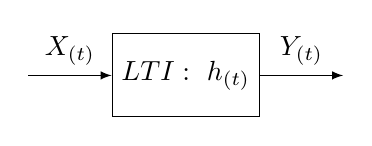
\begin{tikzpicture}[
                        node distance=2cm,
                        >=latex
                    ]
                    % Blocks
                    \node [coordinate] (input) {};
                    \node [rectangle, draw,minimum height=3em, minimum width=3em,right of=input] (filter) {$LTI:\ h_{(t)}$};
                    \node [coordinate, right of=filter] (output) {$s_{(t)}$};
                
                    % Connections
                    \draw [->] (input) --node[above]{$X_{(t)}$} (filter);
                    \draw [->] (filter) --node[above]{$Y_{(t)}$} (output);
                \end{tikzpicture}    
            \end{figure}
            l'uscita $Y_{(t)}$ si calcola con la convoluzione:
            \[
                Y_{(t)} = X_{(t)} \otimes h_{(t)} = \int_{-\infty}^{\infty} X_{(\alpha)} h_{(t-\alpha)} d\alpha
            \]
            Calcolaimone gli indici:
            \begin{itemize}
                \item {
                    Valore medio:
                    \begin{align}
                        \mu_Y &= \mathbb{E}[Y_{(t)}] =\mathbb{E}[X_{(t)} \otimes h_{(t)}] = \mathbb{E}\left[\int_{-\infty}^{\infty} X_{(\alpha)} h_{(t-\alpha)} d\alpha\right]\nonumber \\
                              &\overset{\ref{linearita expectation}}{=} \int_{-\infty}^{\infty} \mathbb{E}[X_{(\alpha)}] h_{(t-\alpha)} d\alpha = \int_{-\infty}^{\infty} \mu_{X_{(\alpha)}} h_{(t-\alpha)} d\alpha  \nonumber \\
                              &=  \mu_{X_{(t)}} \otimes h_{(t)}\nonumber
                    \end{align}
                }
                \item {
                    Autocorrelazione:
                    \begin{align}
                        R_{YY(t_1,t_2)} &= \mathbb{E}[Y_{(t_1)}Y_{(t_2)}] = \mathbb{E}\left[\int_{-\infty}^{\infty} X_{(\alpha_1)} h_{(t-\alpha_1)} d\alpha_1\int_{-\infty}^{\infty} X_{(\alpha_2)} h_{(t-\alpha_2)} d\alpha_2\right]\nonumber \\
                                        &= \int_{-\infty}^{\infty}\int_{-\infty}^{\infty} \mathbb{E}[X_{(\alpha_1)}X_{(\alpha_2)}] h_{(t-\alpha_1)} h_{(t-\alpha_2)} d\alpha_1d\alpha_2\nonumber \\
                                        &\overset{C. Var.}{=} R_{X(t_1,t_2)} \otimes h_{(t_1)}\otimes h_{(t_2)}\nonumber
                    \end{align}
                }
            \end{itemize}
            Supponiamo adesso che il processo $X_{(t)}$ sia SSL, verifchiamo se anche $Y_{(t)}$ é SSL:
            \paragraph{Valore Medio:}
                \begin{align}
                    \mu_Y &= \mathbb{E}[Y_{(t)}] = \int_{-\infty}^{\infty} \mathbb{E}[X_{(\alpha)}] h_{(t-\alpha)} d\alpha = \int_{-\infty}^{\infty} \mu_{X_{(\alpha)}} h_{(t-\alpha)} d\alpha \nonumber \\
                            &= \mu_{X_{(\alpha)}} \int_{-\infty}^{\infty} h_{(t-\alpha)} d\alpha \overunderset{\beta = t-\alpha}{d\beta = -d\alpha}{=} \mu_{X_{(\alpha)}} \int_{-\infty}^{\infty} h_{(\beta)} d\beta\nonumber \\
                            &= \mu_X H_{(0)}\nonumber
                \end{align}
                si $H_{(0)}$ é proprio il grande ritorno di una $TCF$, viene fuori perché se calcoliamo la $TCF$ in $0$
                \[
                    \eval*{\int_{-\infty}^{\infty} h_{(\beta)} e^{-j2\pi f\beta} d\beta}_{f = 0} = \int_{-\infty}^{\infty} h_{(\beta)} d\beta = H_{(0)}
                \]
                il quale coincide con il valore medio.
            \paragraph{Autocorrelazione:}
                \begin{align}
                    R_{Y(t_1,t_2)} &= R_{X(\tau)}\otimes h_{(\tau)} \otimes h_{(-\tau)} \nonumber \\
                                    &= \int_{-\infty}^{\infty}\int_{-\infty}^{\infty} h_{(\tau_1)}h_{(\tau_2)} R_{XX(\tau+\tau_1-\tau_2)} d\tau_1d\tau_2\nonumber
                \end{align}    
        \subsubsection{Densitá di potenza spettrale}
            Supponiamo di voler caratterizzare l'output di $Y_{(t)}$ usando il dominio della frequenza:
            \[
                \mathbb{E}[Y_{(t)}^2] = \int_{-\infty}^{\infty} \left|H_{(f)}\right|^2 S_{XX(f)} df  
            \]
            dove $S_{XX(f)}$ é la Densitá di potenza spettrale:
            \[
                S_{XX(f)} = \int_{-\infty}^{\infty} R_{XX(\tau)} e^{-j2\pi f\tau}d\tau
            \]
            ma perché menziona la potenza?
            \begin{align}
                P_x &= \mathbb{E}[X^2] = R_{X(0)} \overset{ATCF[S_{X(f)}]}{=} \eval*{\int_{-\infty}^{\infty} S_{X(f)} e^{j2\pi f\tau}df}_{\tau=0} \nonumber \\
                    &=  \int_{-\infty}^{\infty} S_{X(f)}df \nonumber
            \end{align}
            trovo la relazione per l'uscita $Y_{(t)}$:
            \begin{figure}[H]
                \centering
                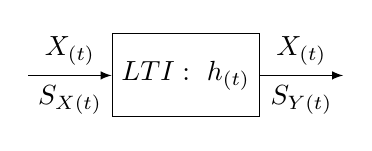
\begin{tikzpicture}[
                        node distance=2cm,
                        >=latex
                    ]
                    % Blocks
                    \node [coordinate] (input) {};
                    \node [rectangle, draw,minimum height=3em, minimum width=3em,right of=input] (filter) {$LTI:\ h_{(t)}$};
                    \node [coordinate, right of=filter] (output) {$s_{(t)}$};
                
                    % Connections
                    \draw [->] (input) --node[above]{$X_{(t)}$} node[below]{$S_{X(t)}$} (filter);
                    \draw [->] (filter) --node[above]{$X_{(t)}$} node[below]{$S_{Y(t)}$} (output);
                \end{tikzpicture}    
            \end{figure}            
            \begin{align}
                S_{Y(f)} &= TCF[R_X] =TCF[ R_{X(\tau)}\otimes h_{(\tau)} \otimes h_{(-\tau)}] \overset{\ref{Conv. Distributiva}}{=}  S_{X(f)}H_{(f)} H_{(-f)}    \nonumber \\
                         &\overset{\ref{Simmetria Hermitiana}}{=} S_{X(f)}H_{(f)} H^\ast_{(f)} =  S_{X(f)}|H_{(f)}|^2\nonumber
            \end{align}
            trovo che la denitá spettrale di potenza di $Y_{(t)}$ é la densitá spettrale di potenza di $X_{(t)}$ per il modulo quadro della
            risposta del filtro e la sua misura é in watt per hertz ($W/Hz$).
    \subsection{Processo Gaussiano}
        Un processo $Y_{(t)}$ é detto processo Gaussiano se la variabile aleatoria $Y$ é una variabile aleatoria a distribuzione Gaussiana:
        \[
            f_{Y(y)} = \frac{1}{\sqrt{2\pi}\sigma}e^{\left(\displaystyle-\frac{(y-\mu)^2}{2\sigma^2}\right)}    
        \] 
        \paragraph{Propietá:}
        \begin{itemize}
            \item {
                Il processo stocastico creato da un fenomeno fisico solitamente é possibile ricondurlo a un modella Gaussiano.
            }
            \item {
                L'uso di un modello Gaussiano per un fenomeno fisico é spesso confermato dagli esperimenti.
            }
            \item {
                Il teorema del limite centrale (\ref{Teorema del Limite Centrale - Central Limit Theorem}) fornisce una giustificazione matematica per la 
                distribuzione Gaussiana.
            }
        \end{itemize}
        \subsubsection{Rumore Bianco}
            É una sorgente di rumore idealizzata in modo tale da rendere lo spettro di densitá di potenza costante ($\frac{N_0}{2}$), cioé indipendente
            dalla frequenza a cui operiamo. L'aggettivo "Bianco" deriva dall'ottica: un segnale di luce bianca contine in ugual maniera tutte le frequenze
             all'interno dello spettro visivo. Ne possiamo dare una definizione approssimativa:
             \begin{center}
                Il rumore bianco, identificato da $W_{(t)}$ é un processo stazionario con densitá di potenza spettrale $S_{W(f)}$ con valore
                costante in tutto l'intervallo delle frequenze:
                \[
                    S_{WW(f)} = \frac{N_0}{2}\ \forall f  
                \]
             \end{center}
             \begin{figure}[H]
                \centering
                \subfloat[Densitá di potenza spettrale]{
                    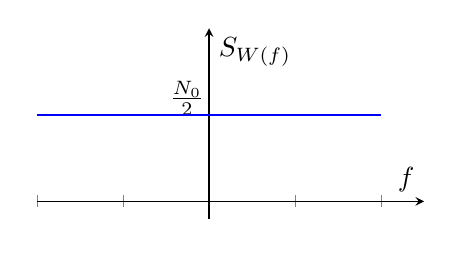
\begin{tikzpicture}
                        \begin{axis}[
                            xlabel=$f$,
                            ylabel=$S_{W(f)}$,
                            xmin=-4,
                            xmax=5,
                            ymin=-0.2,
                            ymax=2,
                            ytick = {1},
                            xtick={},
                            xticklabels={},
                            yticklabel style = {yshift=6pt,xshift=4pt}, 
                            yticklabels = {$\frac{N_0}{2}$},
                            axis lines=middle,
                            domain=-4:4,
                            samples=100,
                            width=6.5cm,
                            height=4cm
                        ]
                        \addplot [const plot, blue, thick] coordinates{(-4,1)(4,1)};
                        \end{axis}
                    \end{tikzpicture}
                }
                \hfill
                \subfloat[Autocorrelazione]{
                    \begin{tikzpicture}
                        \begin{axis}[
                            xlabel=$\tau$,
                            ylabel=$R_{X(\tau)}$,
                            xmin=-4,
                            xmax=5,
                            ymin=-0.2,
                            ymax=2,
                            ytick = {1},
                            xtick={},
                            xticklabels={},
                            yticklabel style = {yshift=5pt,xshift=4pt}, 
                            yticklabels = {$\frac{N_0}{2}\delta_{(\tau)}$},
                            axis lines=middle,
                            domain=-5:5,
                            samples=100,
                            width=6.5cm,
                            height=4cm
                        ]
                        \addplot+ [blue, thick,mark = triangle] coordinates{(0,0)(0,1)};
                        \end{axis}
                    \end{tikzpicture}
                }
            \end{figure}
            \paragraph{Propietá:}
            \begin{itemize}
                \item {Dato che $R_{W(\tau)}=0\ \forall \tau\neq 0$ ne segue che due differenti campionamenti del rumore bianco sono completamente
                incorrelati tra loro}
                \item {
                    Se il rumore bianco é Gaussiano allore due campioni sono statisticamente indipendenti.
                }
                \item {
                    Finché la banda di un processo del rumore in ingresso al sistema é ampiamente maggiore della banda del sistema stesso, allora possiamo modellare
                    il rumore come un processo a rumore bianco.
                }
            \end{itemize}
        \subsubsection{Filtro passa basso ideale per rumore bianco}
            Supponiamo di avere un ricevitore:
            \begin{figure}[H]
                \centering
                    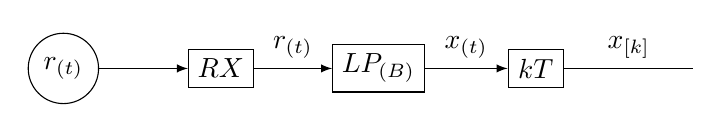
\begin{tikzpicture}[
                            node distance=2cm,
                            >=latex
                        ]
                        % Blocks
                        \node [circle,draw] (RXant) {$r_{(t)}$};
                        \node [rectangle, draw,minimum height=1em, minimum width=2em,right of=RXant] (RX) {$RX$};
                        \node [rectangle, draw,minimum height=1em, minimum width=2em,right of=RX] (DC) {$LP_{(B)}$};
                        \node [rectangle, draw,minimum height=1em, minimum width=2em,right of=DC] (DS) {$kT$};
                        \node [coordinate,right of = DS] (output) {};
                    
                        % Connections
                        \draw [->] (RXant) --node[above]{} (RX);
                        \draw [->] (RX) --node[above]{$r_{(t)}$} (DC);
                        \draw [->] (DC) --node[above]{$x_{(t)}$} (DS);
                        \draw [-] (DS) --node[above]{$x_{[k]}$} (output);
                    \end{tikzpicture}    
            \end{figure}
            e un rumore additivo:
            \begin{figure}[H]
                \centering
                    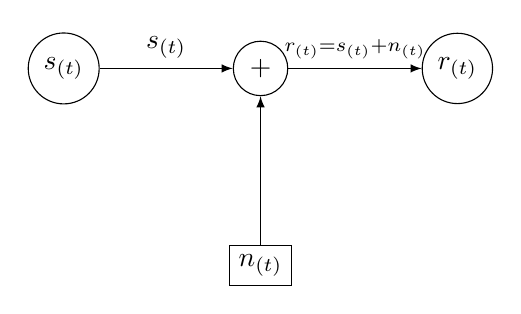
\begin{tikzpicture}[
                            node distance=2.5cm,
                            >=latex
                        ]
                        % Blocks
                        \node [circle,draw] (TXant) {$s_{(t)}$};
                        \node [circle, draw,right of=TXant] (sum) {$+$};
                        \node [rectangle, draw,below of = sum,minimum height=1em, minimum width=2em] (error) {$n_{(t)}$};
                        \node [circle,draw,right of=sum] (RXant) {$r_{(t)}$};
                    
                        % Connections
                        \draw [->] (TXant) --node[above]{$s_{(t)}$} (sum);
                        \draw [->] (sum) --node[above]{$\scriptstyle r_{(t)} = s_{(t)}+ n_{(t)}$} (RXant);
                        \draw [->] (error) -- (sum);
                    \end{tikzpicture}    
            \end{figure}
            inviamo un segnale $s_{(t)}$ con banda $B$:
            \begin{figure}[H]
                \centering
                \subfloat[Trasmettitore]{
                    \begin{tikzpicture}
                        \begin{axis}[
                            xlabel=$f$,
                            ylabel=$S_{W(f)}$,
                            xmin=-5,
                            xmax=5,
                            ymin=-0.2,
                            ymax=1,
                            ytick = {1},
                            xtick={-2,2},
                            xticklabels={$-B$,$B$},
                            yticklabel style = {yshift=6pt,xshift=4pt}, 
                            yticklabels = {$\frac{N_0}{2}$},
                            axis lines=middle,
                            domain=-5:5,
                            samples=800,
                            width=6.5cm,
                            height=4cm
                        ]
                        \addplot [const plot, blue, thick, domain = -2:2] {gauss(0,0.8)-0.01};
                        \end{axis}
                    \end{tikzpicture}
                }
                \hfill
                \subfloat[Ricevitore: ${\color{blue}s_{(t)}}+ {\color{purple}n_{(t)}}$]{
                    \begin{tikzpicture}
                        \begin{axis}[
                            xlabel=$\tau$,
                            ylabel=$R_{X(\tau)}$,
                            xmin=-5,
                            xmax=5,
                            ymin=-0.2,
                            ymax=1,
                            ytick = {1},
                            xtick={-2,2},
                            xticklabels={$-B$,$B$},
                            yticklabel style = {yshift=5pt,xshift=4pt}, 
                            yticklabels = {$\frac{N_0}{2}\delta_{(\tau)}$},
                            axis lines=middle,
                            domain=-5:5,
                            samples=800,
                            width=6.5cm,
                            height=4cm
                        ]
                        \addplot [const plot, blue, thick, domain = -2:2] {gauss(0,0.8)-0.01};
                        \addplot [const plot, purple, thick] coordinates{(-5,0.2)(5,0.2)};
                    \end{axis}
                    \end{tikzpicture}
                }
                \
            \end{figure}
            il ricevitore si occupa adesso del filtraggio con un filtro passa basso di banda $B$ ($LP_{(B)}$), ritrovando il 
            segnale originale ma con il rumore additivo:
            \begin{figure}[H]
                \centering
                \begin{tikzpicture}
                    \begin{axis}[
                        xlabel=$\tau$,
                        ylabel=$R_{X(\tau)}$,
                        xmin=-5,
                        xmax=5,
                        ymin=-0.2,
                        ymax=1,
                        ytick = {0.6},
                        xtick={-2,2},
                        xticklabels={$-B$,$B$},
                        yticklabel style = {yshift=5pt,xshift=4pt}, 
                        yticklabels = {$1$},
                        axis lines=middle,
                        domain=-5:5,
                        samples=800,
                        width=8cm,
                        height=5cm
                    ]
                    \addplot [const plot, blue, thick, domain = -2:2] {gauss(0,0.8)-0.01};
                    \addplot [const plot, purple, thick] coordinates{(-5,0.2)(5,0.2)};
                    \addplot [const plot, orange, thick] coordinates{(-5,0)(-2,0)(-2,0.6)(2,0.6)(2,0)(5,0)};
                \end{axis}
                \end{tikzpicture}
                \caption{${\color{blue}s_{(t)}},{\color{purple}n_{(t)}},{\color{orange}LP-filter}$}
            \end{figure}
            in uscita dal filtro ho $x_{(t)} = s_{(t)} + n_{(t)} \otimes h_{(t)}$ con la densitá spettrale del rumore:
            \[
                S_{W(f)} = S_{n(f)} |H_{(f)}|^2 = S_{n(f)} 
            \]
            Per ricostruire il segnale devo campionare con una $f_s = \frac{1}{T_s} = 2B$ ($kT$):
            \[
                x_{[k]} = x_{(t=kT)} = s_{[k]}+w_{[k]}    
            \]
            Cosa succede al rumore? MA POSSO CAMBIARE SPETTRO E TCF NE GRAFO?
            Nel dominio della frequenza lo spettro di rumore filtrato,$w_{[k]}$, é  una somma di delta di dirac ho quindi $S_{w(f)} = rect\left(\frac{f}{2B}\right)$
            trasformadola nel dominio del tempo, cio;e calcolando la sua autocorrelazione per $ATCF[S_{w(f)}] = R_{w(\tau)}$ ottengo $R_{w(\tau)} = 2B\tau sinc(2B\tau)$,
            campionandola conrispetto alla banda del filtro $B$ in $\frac{k}{2B}$ la $sinc$ é sempre $0$ rendendo le variabili del rumore Gaussiano statisticamente 
            indipendenti a valore medio nullo e varianza $N_0B$. 
            \[
                \eval*{R_{w(\tau)}}_{\tau=kT} =\eval*{\mathbb{E}[w_{(t)}w_{(t-\tau)}]}_{\tau=kT} \overset{T=\frac{1}{2B}}{=} 0  
            \]
            \begin{figure}[H]
                \centering
                \begin{tikzpicture}
                    \begin{axis}[
                        xlabel=$\tau$,
                        ylabel=$R_{X(\tau)}$,
                        xmin=-5,
                        xmax=5,
                        ymin=-1,
                        ymax=1.5,
                        ytick={1},
                        yticklabels = {$N_0B$},
                        yticklabel style = {yshift=5pt,xshift=4pt}, 
                        xtick={-4,-3,-2,-1,1,2,3,4},
                        xticklabels={$-\frac{4}{2B}$,$-\frac{3}{2B}$,$-\frac{2}{2B}$,$-\frac{1}{2B}$,$\frac{1}{2B}$,$\frac{2}{2B}$,$\frac{3}{2B}$,$\frac{4}{2B}$},
                        xticklabel style = {yshift=-3pt}, 
                        axis lines=middle,
                        domain=-5:5,
                        samples=800,
                        width=10cm,
                        height=6cm
                    ]
                    \addplot [blue, thick, samples = 800] {sin(deg(x*pi))/(x*pi)};
                \end{axis}
                \end{tikzpicture}
            \end{figure}
            per questo il modello $Y = S + n \sim \mathcal{N} (0,\sigma^2)$ é giusto per approssimare il rumore.










    \section{Teoria Dei Codici}
    \subsection{Introduzione}
        Ci concentriamo adesso sul trattamento dell'informazione per poterla trasmettere.
        I messaggi che trasmettiamo possono essere codificati per vari motivi:
        \begin{itemize}
            \item {
                    Compressione:$\begin{cases}
                        \text{Lossy: con perdita dell'informazione} \nonumber\\
                        \text{Lossless: minima perdita dell'informazione} \nonumber
                    \end{cases}$\\
                    Comprimere l'informazione in elimenando ridondanza e salvando spazio di memoria e banda.
                    
                }
            \item {
                    Crittografia: per nascondere il messaggio ad utenti in ascolto sul canale che non siano il destinatario.
            }
            \item {
                    Rivelazione o correzione di errore: vieen aggiunta ridondanza ad hoc per aumentare l'affidabilitá del messaggio trasmesso. 
                    Si utilizzano \href{https://en.wikipedia.org/wiki/Checksum}{checksum} o \href{https://en.wikipedia.org/wiki/Reed-Solomon_error_correction}{Reed-Solomon(RS)}
            }
        \end{itemize}
        \paragraph{Capacitá del canale}\label{Capacita del canale}\index{Capacitá del canale}
            La capacitá del canale $C$ indica la massima quantitá d'informazione che puó essere trasmessain maniera affidabile su di un dato canale.
            La capacitá dipende dalla banda $B$ del canale e dal rapporto segnale rumore (signal-to-noise ratio,\href{https://en.wikipedia.org/wiki/Signal-to-noise_ratio}{$SNR$}):
            \[
                C = B\log(1 + SNR)  
            \] 
        \paragraph{Canale Gaussiano}\index{Canale Gaussiano}
            Il canale Gaussiano puó essere modellato come \href{https://en.wikipedia.org/wiki/Binary_symmetric_channel}{Binary Symmetric Channel (BSC)} con probabilitá di errore $p$. 
            Assumiamo gli errori tra loro indipendenti ($p_{(a,b)} = p_{(a)}\dotproduct p_{(b)}$):
        \begin{figure}[H]
            \centering
            \includegraphics[width = 12cm]{media/600px-Binary_symmetric_channel_(en).svg.png}
            \label{BSC system}
            \caption{Sistema di trasmissione BSC}
        \end{figure}
        \begin{gather}
            E_{(x)}: \text{Funzione di codifica} \nonumber \\
            D_{(x)}: \text{Funzione di decodifica} \nonumber \\
            E_{(m)}: \text{Bit dell'informazione codificati} \nonumber \\
            y^\prime: E_{(m)}+ e \rightarrow \text{Informazioni con errore del canale} \nonumber \\
            m = D_{(y^\prime)}: \text{Informazione decodificata} \nonumber 
        \end{gather}
        Il canale é chiamato simmetrico perché ho la stessa probabilitá errore sulla trasmissione di uno dei due bit.
        Se $X$ é il bit inviato e Y quello ricevuto allora il canale é caratterizzato dalle probabilitá:
        \begin{align}
            P(Y=0|X=0) &= 1-p\nonumber \\
            P(Y=0|X=1) &= p\nonumber \\
            P(Y=1|X=0) &= p\nonumber \\
            P(Y=1|X=1) &= 1-p\nonumber 
        \end{align} 
        Assumiamo che $0\leq p \leq\frac{1}{2}$, se avessimo $p >\frac{1}{2}$ il ricevitore potrebbe scambiare l'informazione ricevuta
        (Quando riceve un $1$ lo interpreta come $0$ e viceversa) e ottenere un canale con probabilitá $1-p \leq\frac{1}{2}$. 
        
        Nel corso useremo delle simbologie diverse:
        \begin{figure}[H]
            \centering
            \includegraphics[width = 12cm]{media/BSC System.png}
            \label{BSC system moretti}
            \caption{Sistema di trasmissione BSC}
        \end{figure}
        \begin{gather}
            u: \text{Informazione} \nonumber \\
            x: \text{Parole di Codice} \nonumber \\
            e: \text{Errore del Canale} \nonumber \\
            y: x+e \rightarrow \text{Informazioni con errore del canale} \nonumber \\
            \overset{\wedge}{x}: \text{Informazione decodificata} \nonumber 
        \end{gather}
        \paragraph{Probabilitá di errore BSC}\label{Probabilita di errore BSC}\index{Probabilitá di errore BSC}
            La probabilitá, per una trasmissione BSC, di sbagliare $t$ bit in una parola di $n$ bit:
            \[
                p_{(t,n)} = \binom{n}{t} p^t (1-p)^{(n-t)}
            \]
            dove il coefficente binomiale:
            \[
                \binom{n}{t} = \frac{n!}{t!(n-t)!}
            \]
            indica tutte le possibili combinazioni di errori di $t$ bit su $n$ bit. 
        \paragraph{Tassonomia dei codici}
            \begin{itemize}
                \item {Codici lineari
                        \begin{itemize}
                            \item {
                                Codici a blocco
                                }
                            \item{
                                Codici convoluzionali
                            } 
                        \end{itemize}
                    }
                \item {
                    Definizione di un codice a blocco: 
                    \begin{figure}[H]
                        \centering 
                        \begin{tikzpicture}[
                            node distance=2cm,
                            >=latex
                            ]

                            \node [coordinate] (input) {};
                            \node [draw, rectangle,right of = input, minimum height=3em, minimum width=6em] (block) {$x_{(t)}$};
                            \node [coordinate, right of = block] (output) {};
                            
                            \draw[draw,->] (input) -- node[midway]{$/$} node[below]{$k$} (block);
                            \draw[->] (block) -- node[midway]{$/$} node[below]{$n$} (output);
                        \end{tikzpicture}    
                    \label{Def codice a blocco}
                    \end{figure}
                    \paragraph{Rate del Codice}:\index{Rate del Codice}
                        {
                            \[
                                R = \frac{k}{n}  
                            \]
                            La condizione é che $n>k$ senon fosse cosí avrei perdita d'informazione, da $k$ bit passo a $n$ aggiungendo
                            ridondanza e codificando i miei dati. Possiamo quindi stimare il valore tipico di $R$
                            \[
                                R = \frac{k}{n} <1  
                            \]
                        }
                }
                \item Rivelazione di errore:\index{Rivelazione di errore}{
                    Consiste nella capacità di scoprire la presenza di errori causati dal rumore o da altri fenomeni deterioranti 
                    durante una trasmissione di dati (es. tramite il \href{https://it.wikipedia.org/wiki/Bit_di_parit%C3%A0}{bit di paritá}).
                }
                \item {Correzione di errore:\index{Correzione di errore}{
                    Consiste invece nell'ulteriore abilità di ricostruire i dati originali, eliminando gli errori occorsi durante la trasmissione.
                    Vi sono due differenti schemi di base per la progettazione della codifica di canale e del protocollo per un sistema che corregge gli errori:
                    \begin{itemize}
                        \item {
                            ??\href{https://it.wikipedia.org/wiki/Automatic_repeat-request}{Automatic repeat-request} (ARQ): Il mittente invia i dati ed anche un codice a rilevazione d'errore, che sarà
                            utilizzato in ricezione per individuare gli eventuali errori, ed in tal caso chiedere la ritrasmissione dei dati
                            corrotti. In molti casi la richiesta è implicita; il destinatario invia un acknowledgement (ACK) di corretta 
                            ricezione dei dati, ed il mittente re-invia solo quei dati per i quali non ha ricevuto, entro un prefissato tempo 
                            limite (timeout), il corrispondente ACK.
                        }
                        \item{
                            ??\href{https://it.wikipedia.org/wiki/Forward_Error_Correction}{Forward Error Correction} (FEC): Il mittente codifica i dati con un codice a correzione d'errore 
                            (error correction code, ECC) ed invia il messaggio codificato. Il destinatario non invia mai alcun 
                            messaggio verso il mittente; esso decodifica ciò che riceve nella maniera più simile possibile a quella di un 
                            certo insieme prefissato di parole accettabili. Tali codici sono realizzati in modo tale che dovrebbe occorrere 
                            una quantità "irragionevole" di errori nei dati, affinché il destinatario decodifichi erroneamente, ottenendo 
                            finalmente dei dati diversi da quelli effettivamente inviatigli.
                        } 
                    \end{itemize}
                    In generale un codice a blocco che ha rate $\frac{k}{n}$ mappa $k$ bit su $n$ bit usando $2^k$ parole di codice di dimensione n
                }}
            \end{itemize}

        \subsubsection{Esempio codici a blocco: codici a ripetizione}
            É un esempio di codice a correzione d'errore: il funzionamento si basa sulal ripetizione dell'informazione piú volte. Il destinatario
            si accorge di un errore di trasmissione poiché il flusso di dati ricevuto non è la ripetizione di un singolo messaggio e, inoltre, 
            il destinatario può recuperare il messaggio originale guardando il messaggio ricevuto nel flusso di dati che si verifica più spesso.

            Nel caso di un codice binario di ripetizione, esistono due parole in codice - tutte uno e tutti zeri - che hanno una lunghezza n. 
            Pertanto, la distanza minima di Hamming (\ref{Distanza di Hamming}) del codice è uguale alla sua lunghezza. Ciò conferisce al codice 
            di ripetizione, con $R = \frac{1}{n}$,una capacità di rivelazione di errori pari a $n-1$ e correzione degli errori (cioè correggerà fino agli errori in qualsiasi parola del codice) di $\frac{n-1}{2}$ per n dispari(\ref{Probabilita di errore BSC}).\\
            Esempio:\\
            \indent{$R = \frac{1}{3} \rightarrow$ ha solo 2 parole di codice:}
            \begin{align}
                u=0 \rightarrow x = [000]\nonumber \\
                u=1 \rightarrow x = [111]\nonumber
            \end{align} 
            Il ricevitore effettua una decodifica a maggioranza: decide per il bit che comprare piú volte della parola ricevuta.
            \begin{align}
                y = [000] \rightarrow \overset{\wedge}{x} = [000] \rightarrow \overset{\wedge}{u} = 0 \nonumber \\
                y = [010] \rightarrow \overset{\wedge}{x} = [000] \rightarrow \overset{\wedge}{u} = 0 \nonumber \\
                y = [101] \rightarrow \overset{\wedge}{x} = [111] \rightarrow \overset{\wedge}{u} = 1 \nonumber
            \end{align}
            \paragraph{Evento errore:} l'evento errore per un codice a correzione di errore consiste nel non essere in grado di correggere
            tutti gli errori introdotti dal canale. Se la probabilitá di errore sul bit $p_{e,b}$ é piccola, la probabilitá di errore 
            $p_{e,W}$ per il codice puó essere approssimata dal primo evento che determina la ricezione errata (nel caso dei codici a ripetizione a $R = \frac{1}{3}$ 
            si verifichino $2$ errori).
            \begin{itemize}
                \item {$R = \frac{1}{3}$
                    \begin{itemize}
                        \item {
                            Se $p_{e,b} = 0.1 \Rightarrow p_{e,W} \approx 2.7\dotproduct 10^{-2} $ 
                        }
                        \item {
                            Se $p_{e,b} = 0.01 \Rightarrow p_{e,W} \approx 2.97\dotproduct 10^{-4} $ 
                        }
                    \end{itemize}
                }
                \item {$R = \frac{1}{5}$
                    \begin{itemize}
                        \item {
                            Se $p_{e,b} = 0.1 \Rightarrow p_{e,W} \approx 8.1\dotproduct 10^{-3} $ 
                        }
                        \item {
                            Se $p_{e,b} = 0.01 \Rightarrow p_{e,W} \approx 9.8\dotproduct 10^{-6} $, Sviluppiamo i calcoli come esempio: 
                            \[
                                P_r \{\text{codice }R=\frac{1}{5}\text{ non riesce a correggere gli errori introdotti dal canale}\}:
                            \]
                            \begin{align}
                                P_r &= \sum_{t=3}^{5} \binom{5}{t}p^t (1-p)^{5-t},\hspace{0.2cm} p=10^{-2} \nonumber \\
                                P_r &\{\text{3 errori su 5}\}= \binom{5}{3}p^3 (1-p)^{5-3} = 10\dotproduct 10^{-6} (0.99)^2 = 9.8\dotproduct 10^{-6} \nonumber \\
                                P_r &\{\text{3 errori su 5}\}= \binom{5}{4}p^4 (1-p)^{5-4} = 5\dotproduct 10^{-8} (0.99) = 5\dotproduct 10^{-8}\nonumber \\
                                P_r &\{\text{3 errori su 5}\}= \binom{5}{5}p^5 (1-p)^{5-5} = 1\dotproduct 10^{-10} = 10^{-10}\nonumber 
                            \end{align}
                        }
                    \end{itemize}
                }
            \end{itemize}

        \subsubsection{Esempio codici a blocco: codici a controllo di paritá}
        Il bit di parità è un codice di controllo d'errore, utilizzato nei calcolatori per prevenire errori nella trasmissione o nella memorizzazione dei dati. 
        Tale codice prevede l'aggiunta di un bit ridondante ai dati, calcolato a seconda che il numero di bit che valgono 1 sia pari o dispari. Ne esistono
        quindi 2 varitá: bit di paritá pari e bit di paritá dispari. Quando si usa il bit di paritá pari si aggiunge un bit con valore $1$ se nella parola inviata
        il numero di occorrenze di "$1$" é dispari(portando il numero di occorrenze di "$1$" a una quantitá pari).Quando si usa il bit di paritá dispari si
        aggiunge un bit con valore $1$ se nella parola inviata il numero di occorrenze di "$1$" é pari (portando il numero di occorrenze di "$1$" a una quantitá dispari).

        \noindent Il codice ha $R = \frac{k}{(k+1)}$: $k$ bit informativi piú il bit di paritá.
        
        \paragraph{Rilevazione dell'errore:}La rilevazione d'errore deriva dalla discordanza del numero di occorrenze di "$1$", eseguendo lo XOR bit a bit, nel caso del bit di paritá pari, se il risultato
        é $0$ non sono avvenuti errori, viceversa se ho un risultato uguale a $1$ posso dire che cé stato uno o una quantitá dispari di errori nella trasmissione, questo lo rende
        solo un codice a rilevazione d'errore e non un codice a correzione d'errore.
        
        Esempio:Trasmetto parole di $11bit$ con rate $R_b = 10Mb/s$ e probabilitá di errore sul bit trasmesso $p_{e,b} = 10^{-8}$:
        \begin{itemize}
            \item {
                Senza controllo di paritá é sufficiente che sia sbagliato anche un solo bit per sbagliare tutta la parola:
                \[
                    p_{e,W} = \sum_{j=1}^{11} \binom{11}{j}p_{e,b}^j (1-p_{e,b})^{11-j} = 11 p_{e,b} (1-p_{e,b})^{10} \simeq 11p_{e,b}
                \]
                ed il rate di parole sbagliate al secondo é:
                \[
                    R_{e,W} = \frac{R_b}{11}\dotproduct p_{e,W} \simeq \frac{10^7}{11}\dotproduct 11p_{e,b} = 0.1_\frac{w}{s}
                \]
            }
            \item {
                Aggiungendo un bit di paritá, la parola diventa di 12 bit e sbaglio quando faccio almeno 2 errori, il singolo errore
                viene corretto chiedendo nuovamente la trasmissione del dato:
                \[
                    p_{e,W} = \sum_{j=2}^{12} \binom{12}{j}p_{e,b}^j (1-p_{e,b})^{12-j} = 66 p_{e,b}^2 (1-p_{e,b})^{10} \simeq 66p_{e,b}^2
                \]
                ed il rate (frequenza) di parole sbagliate al secondo é:
                \[
                    R_{e,W} = \frac{R_b}{12}\dotproduct p_{e,W} \simeq \frac{10^7}{12}\dotproduct 66p_{e,b}^2 = 5.5\dotproduct 10^{-9} \frac{w}{s}
                \]
                possiamo anche calcolare il periodo $T_{e,W} = \frac{1}{R_{e,W}} =  1.82\dotproduct 10^{8} s$ che é una parola ogni sei anni circa.  
            }
        \end{itemize}
        \subsubsection{Esempio codici a blocco: codice ISBN}
            Il codice International Standard Book Number (ISBN) é un codice a controllo di paritá per un alfabeto di simboli nonbinari. 
            Ad ogni libro é assegnata una parola di codice di lunghezza $n=10$ cifre in base decimale. Le prime 9 cifre identificano il libro, 
            la decima é quella di controllo di paritá cosí calcolata:
            \begin{enumerate}
                \item {
                    Si calcola la grandezza $z = mod(S,11)$ con
                    \[
                        S = \sum_{j=1}^{9} (11-j)x_{(j)}
                    \]
                }
                \item {
                    La cifra di controllo di aritá é il complemento a 11 di $z$:
                    \[
                        x_{(10)} = mod(11-z,11)  
                    \]
                    E solo per la cifra di controllo di paritá se $x_{(10)} = 10$ si sostituisce con 
                    $x_{(10)} = X$
                }
            \end{enumerate}
            Quando un dispositivo legge il codice lo verifica come segue:
            \begin{enumerate}
                \item {
                    Moltiplica ogni cifra per il peso della posizione della stessa cifra e calcola $mod(S^\prime,11)$ con
                    \[
                        S^\prime = \sum_{j=1}^{10} (11-j)y_{(j)}
                    \]
                }
                \item {
                    Assumendo che non ci siano errori su $x_{(10)} = |11-z|_{11}$, si ha:
                    \begin{align}
                        mod(S^\prime,11) &= mod \left( \sum_{j=1}^{9} (11-j)y_{(j)} + mod(11-z,11),11\right) \nonumber \\
                                         &= mod \left( \sum_{j=1}^{9} (11-j)y_{(j)} + \left(11-\sum_{j=1}^{9} (11-j)x_{(j)}\right),11\right)\nonumber \\
                                         &= mod \left(\sum_{j=1}^{9} (11-j)(y_{(j)}-x_{(j)}),11\right)
                    \end{align}
                }
            \end{enumerate}
            Se non ci sono errori si ha $y=x$ e quindi il $mod(S^\prime,11) = 0$
            \paragraph{Rivalazione degli errori:} Il codice é in grado di rivelare tutti i singoli errori:
            sia $e_{(k)}$ l'errore in posizione $k$,$y_{(k)} = x_{(k)}+ e_{(k)}$:
            \[
                mod(S^\prime,11) = mod((y_{(k)}-x_{(k)})(11-k),11)+mod(e_{(k)}(11-k),11) \neq 0
            \]
            Il codice é in grado di rivelare tutti i casi in cui ci sia uno scambio di 2 cifre del codice. Siano 
            $k_1$ e $k_2$ le 2 posizioni scambiate:
            \begin{align}
                mod(S^\prime,11) &= mod \left((y_{(k_1)}-x_{(k_1)})(11-k_1)+(y_{(k_2)}-x_{(k_2)})(11-k_2),11\right) \nonumber \\
                                 &= mod \left((x_{(k_2)}-x_{(k_1)})(11-k_1)+(x_{(k_1)}-x_{(k_2)})(11-k_2),11\right)\nonumber \\
                                 &= mod \left((x_{(k_2)}-x_{(k_1)})(k_2-k_1),11\right) \neq 0 \nonumber
            \end{align}
            Esempi:
            \begin{itemize}
                \item {Senza errore:
                    \begin{align}
                        ISBN & = 01-333-5485-7 \nonumber \\
                        \left| S^\prime \right|_{11} &= 0\dotproduct 10 +1\dotproduct 9+3\dotproduct 8+3\dotproduct 7+3\dotproduct 6+5\dotproduct 5+4\dotproduct 4+8\dotproduct 3+5\dotproduct 2+7\dotproduct 1\nonumber \\
                        \left| S^\prime \right|_{11} &= \left| 154 \right|_{11} = 0 \nonumber 
                    \end{align}
                    Il codice é corretto 
                }
                \item {Con errore: Scambio le cifre
                    \begin{align}
                        ISBN & = 01-333-5458-7 \nonumber \\
                        \left| S^\prime \right|_{11} &= 0\dotproduct 10 +1\dotproduct 9+3\dotproduct 8+3\dotproduct 7+3\dotproduct 6+5\dotproduct 5+4\dotproduct 4+{\color{red}5\dotproduct 3}+{\color{red}8\dotproduct 2}+7\dotproduct 1\nonumber \\
                        \left| S^\prime \right|_{11} &= \left| 151 \right|_{11} = 8 \neq 0 \nonumber 
                    \end{align}
                    Il codice non é corretto 
                }
            \end{itemize}
        \subsection{Codici a blocco}
        \subsubsection{Introduzione ai codici lineari}
            \paragraph{Campo:} un campo é una struttura composta da un insieme non vuoto $F$ e da due operazioni binarie interne: $\forall \alpha,\beta,\gamma \in F$:
                \begin{itemize}
                    \item {
                        Somma ($XOR$):
                        \begin{itemize}
                            \item {
                                \[
                                    \alpha + \beta = \theta, \theta \in F  
                                \]
                            }
                            \item {Associativa:
                                \[
                                    (\alpha + \beta) + \gamma = \alpha +( \beta + \gamma)
                                \]
                            }
                            \item {Commutativa:
                                \[
                                    \alpha + \beta = \beta + \alpha
                                \]
                            }
                            \item {Elemento Neutro:
                                \[
                                    0\in F,\alpha + 0 = \alpha,\alpha-\alpha = 0
                                \]
                            }
                        \end{itemize}
                    }
                    \item {
                        Prodotto ($AND$):   
                        \begin{itemize}
                            \item {
                                \[
                                    \alpha \dotproduct \beta = \theta, \theta \in F  
                                \]
                            }
                            \item {Associativa:
                                \[
                                    (\alpha \dotproduct \beta) \dotproduct \gamma = \alpha \dotproduct( \beta \dotproduct \gamma)
                                \]
                            }
                            \item {Commutativa:
                                \[
                                    \alpha \dotproduct \beta = \beta \dotproduct \alpha
                                \]
                            }
                            \item {Distributiva:
                                \[
                                    (\alpha + \beta) \dotproduct \gamma = \alpha \dotproduct \gamma + \beta \dotproduct \gamma
                                \]
                            }
                            \item {Elemento Neutro:
                                \[
                                    1\in F,\alpha \dotproduct 1 = \alpha,\forall \alpha \neq 0\rightarrow \alpha\dotproduct\alpha^{-1} = 0
                                \]
                            }
                        \end{itemize}
                    }
                \end{itemize}
        \subsubsection{Campi di Galois}
            Un campo finito, detto anche campo di Galois, é un campo con un numero finito $q$ di elementi. Il numero di elementi di definisce la categoria del
            campo: $GF(2)$ é il campo definito su $\{0,1\}$ con somma modulo 2 ($XOR$) e prodotto modulo 2 ($AND$). Definito lo spazio $GF(2)$ si puó costruire
             lo spazio vettoriale $\mathcal{V}_n=GF(2)^2$, lo spazio di tutti i possibili $2^n$ vettori di $n$ cifre binarie su cui valgono le operazioni definite per 
             $GF(2)$.

        \subsubsection{Codici a blocco lineari su $GF(2)$}
            Sia $u = [u_1, \dots, u_k]$ una generica parola di $k$ cifre binarie. Il codice a blocco lineare $\mathcal{C}(k,n)\subset \mathcal{V}_n$ é l'insieme delle
            $2^k$ parole $x = [x_1, \dots, x_n]$ di $n$ cifre binarie ottenute con la trasformazione lineare:
            \[
                x = uG  
            \]
            Dove $G$ é la matrice generatrice del codice e ha dimensione $k \times n$ di cifre binarie con $n>k$ poiché al massimo
            aggiungo informazioni per la trasmissione, per la correzione o rivelazione d'errore.
            
            Siano $g_i, i = [1, \dots, k]$, le righe di $G$, $x$ é la combinazione lineare delle righe $g_i$:
            \[
                x = \sum_{i=1}^{k}u_ig_i  
            \]
            Per avere $2^k$ parole di codice distinte  é necessario che $G$ abbia rango $k$: le righe di $G$ devono essere linearmente indipendenti e costituiscono 
            una $base$ per il sottospazio vettoriale $\mathcal{C} \subset \mathcal{V}_n$.  

        \subsubsection{Propietá dei codici a blocco lineari}
            Le propietá derivano maggiormente dalla pripietá di linearit;a dei codici:
            \begin{itemize}
                \item {Ogni parola di codice é una combinazione lineare di righe della matrice generatrice.}
                \item {Il codice a blocchi é costituito da tutte le possibili combinazioni delle righe della matrice generatrice.}
                \item {La somma di due parle di codice é ancora una parola di codice.}
                \item {La $n-upla$ di tutti zeri é sempre una parola di codice.}
                \item {Se $x$ é una parola di codice, anche $-x$ é una parol di codice.}
            \end{itemize}

        \subsubsection{Distanza di Hamming}\label{Distanza di Hamming}\index{Distanza di Hamming}
            La distanza di Hamming tra due vettori, o stringhe, $d(x_1,x_2)$ di $n$ elementi é il nuemro di posizioni in cui le due parole
            sono diverse tra loro. Esempi:
            \begin{itemize}
                \item {
                    La distanza di Hamming tra 10{\color{red}1}1{\color{red}1}01 e 10{\color{red}0}1{\color{red}0}01 è 2.
                }
                \item {
                    La distanza di Hamming tra 2{\color{red}14}3{\color{red}8}96 e 2{\color{red}23}3{\color{red}7}96 è 3.
                }
            \end{itemize}
            \paragraph{Peso di Hamming:}\label{Peso di Hamming}\index{Peso di Hamming} Il peso di Hamming,$w(x)$, di una stringa i lunghezza $n$ é la sua distanza di Hamming dal vettore di $n$ zeri,
            $x_0\in \mathcal{V}_n$ é:
            \[
                w(x_0) = d(x_0,0_n)
            \]
            \paragraph{Distanza minima:}\label{Distanza minima}\index{Distanza minima}La distanza minima di un codice $\mathcal{C}$ é la minima distanza di Hamming calcolata fra tutte le possibili parole che appartengono a $\mathcal{C}$.
            \[
                d_{min} (\mathcal{C})= \underset{x_1,x_2 \in \mathcal{C}}{min}d(x_1,x_2)  
            \]
            Per i codici lineari vale che ciascuna parola di codice ha lo stesso insieme di distanze dalle altre parole di codice.
            La distanza minima di un codice si puó calcolare a partire da qualsiasi parola di codice. 
            La distanza di Hamming é una metrica:
            \begin{itemize}
                \item {}
                \item {}
                \item {}
                \item {}
            \end{itemize}
        \subsubsection{Codici a blocco in forma sistematica}
            Quando il codice é in forma sistematica la matrice generatrice del codice ha la seguente forma:
            \begin{gather}
                G = [I_k,P]\nonumber \\
                G\in k\times n,\ I\in k\times k,\ P\in k\times (n-k)\nonumber
            \end{gather}
            dove la matrice $P$ é la matrice di paritá, il suo contenuto dipende da quale algoritmo di paritá viene scelto.
            \begin{figure}[H]
                \centering 
                \begin{tikzpicture}[
                    node distance=2cm,
                    >=latex
                    ]

                    \node [coordinate] (input) {};
                    \node [draw, rectangle,right of = input, minimum height=3em, minimum width=6em] (block) {Coder};
                    \node [coordinate, right of = block] (output) {};
                    
                    \draw[draw,->] (input) -- node[midway]{$/$} node[below]{$k$} (block);
                    \draw[->] (block) -- node[midway]{$/$} node[below]{$n$} (output);
                \end{tikzpicture}    
            \label{Def codice forma sistematica}
            \end{figure}
            \begin{figure}[H]
                \centering 
                \includegraphics[width = 8cm]{media/forma sistematica.png}
            \label{matrice forma sistematica}
            \end{figure}
            \paragraph{Esempio Codice a ripetizione:}
            $R = \frac{1}{3},\ k=1,\ n=3$
            \begin{table}[H]
                \centering
                \begin{tabular}{|c|c|}
                \hline
                Bit i  ingresso & Parola codificata \\ \hline
                0               & {[}000{]}         \\ \hline
                1               & {[}111{]}         \\ \hline
                \end{tabular}
            \end{table}
            La matrice generatirce del codice é $G = [111]$, e la distanza minima $d_{min} = 3$\\

            \paragraph{Esempio Codice a controllo di paritá:}
            $R = \frac{7}{8},\ k=7,\ n=8$, ogni 7 bit ne aggiunge uno di controllo di paritá, 1 se il numero di "1" é diapari,
            0 se il numero di "1" é diapari.


            \noindent La matrice generatirce del codice:
            \[
                G = [I_7,1_7]
            \]
            \noindent La distanza minima é $d_{min} = 2$, se cambio uno dei 7 bit della parola
            cambio automaticamente il bit di paritá, quindi cambiare 1 bit in realtá ne cambia 2.\\

            \noindent Il prodotto $u\dotproduct 1_7 = \sum_{i=1}^{7}u_i$, puó essere scritto come una soma modulo 2, vale 0 se il numero di 
            occorrenze di "1" é pari e 1 altrimenti. Non facciamo altro che calcolare il bit di paritá della parola $u$.
            
            \paragraph{Definizione:} Due codici lineari $\mathcal{C}_1(k,n)$ e $\mathcal{C}_2(k,n)$ in $GF(2)$ sono equivalenti se uno é ottenuto dall'altro
            attraverso una permutazione delle posizioni del codice.

            \paragraph{Teorema:} Due matrici generatrici $G_1$ e $G_1$ in $GF(2)$ generano due codici equivalenti se una puó essere ottenuta dall'altra
            da una sequenza di operazioni come:
            \begin{itemize}
                \item Permutazione delle righe.
                \item Combinazione lineare delle righe.
                \item Permutazione delle colonne.
            \end{itemize}
            
            \paragraph{Teorema:} Qualsiasi codice lineare a blocchi é equivalente ad un codice in forma sistematica.

            \paragraph{Propietá degli spazi:}
            \begin{itemize}
                \item {
                    Dato il sottospazio $\mathcal{C} \subset \mathcal{V}_n$ di dimensione $k$, esiste un sottospazio ortogonale (null space)
                    $\mathcal{C}^\perp \subset \mathcal{V}_n$ di dimensione $n-k$ definito da una matrice $H\in (n-k) \times n$:
                    \[
                        GH^T = 0_{n-k}  
                    \]
                }
                \item {
                    La base di $\mathcal{C}^\perp$ é costituita dalle $n-k$ righe della matrice $H$, per cui ogni elemento $t\in \mathcal{C}^\perp$ puó 
                    essere rappresentato:
                    \[
                        t = vH = \sum_{i=1}^{n-k}v_ih_i  
                    \]
                }
                \item {
                    Per ogni $x\in \mathcal{C}$ e per ogni $t\in \mathcal{C}^\perp$ si ha:
                    \[
                        xt^T = uGH^Tv^T = 0
                    \]  
                }
            \end{itemize}
        \subsubsection{Matrice di controllo di paritá}\label{Matrice di controllo di parita}\index{Matrice di controllo di paritá}
            La matrice $H$ é la matrice di controllo di paritá del codice. Per costruzione $\forall x \in \mathcal{C}$ vale:
            \begin{gather}
                    xH^T = uGH^T = 0 \nonumber \\
                    H\in (n-k) \times n\nonumber 
            \end{gather}
            La matrice $H$ non é unica, ma se il codice é sistematico posso ricavarla in un'altra forma:
            \begin{gather}
                H = [P^T,I_{n-k}] = 0 \nonumber \\
                H\in (n-k) \times n,\ I\in (n-k)\times (n-k),\ P^T\in (n-k) \times k \nonumber
            \end{gather}
            Se fosse $\neq 0$ ció che é stato ricevuto non é una parola di codice.
            
            \paragraph{Esempio codice a ripetizione e controllo di paritá:}
                $R = \frac{1}{3},\ k=1,\ n=3,\ n-k=2$ ho la matrice a controllo di paritá:
                \[
                    H= [P^T,I_2] =
                        \begin{bmatrix}
                        1 & 1 & 0\\
                        1 & 0 & 1
                        \end{bmatrix}  
                \]  
                Per un codice con $R = \frac{7}{8},\ k=7,\ n=8,\ n-k=1$ la matrice a controllo di paritá:
                \[
                    H= [P^T,I_1] = 1_8^T
                \]
        \subsubsection{Propietá dei codici a blocco}
            \paragraph{Teorema:} La distanza minima del codice a blocco $\mathcal{C}(k,n)$ si puó calcolare come il 
            peso di Hamming minimo tra tutte le parole di codice:
            \begin{align}
                d_{min}(\mathcal{C}) &= \underset{x_i,x_j\in\mathcal{C}}{\min} d_H(x_i,x_j) = \underset{x_i,x_j\in\mathcal{C}}{\min} d_H(x_i+x_j,x_j+x_j)\nonumber \\
                                     &= \underset{x_i,x_j\in\mathcal{C}}{\min} d_H(x_i+x_j,0_{1,n}) \overset{[x_i+x_j\in\mathcal{C}]}{\Rightarrow} \underset{x_i\in\mathcal{C}}{\min}\ w(x_i)\nonumber
            \end{align}
            \paragraph{Capacitá di rivelare errori (Error Detection):}
                Su un canale $BSC$ senza memoria (\ref{BSC system moretti}), la $n-upla\ y$ a valle del decisore puó essere rappresentata:
                \[
                    y=x+e  
                \] 
                Dove $e$ é il vettore di errori introdotto dal canale, se il canale non introduce errori: $e = 0_{1,n}$
                Sia $x$ la parola di codice trasmessa e $y=x+e$ la corrispondente sequenza di $n$ bit ricevuta. supponiamo che il canale 
                introduca un numero di errori:$w(e) > 0$, si dice:
                \begin{itemize}
                    \item {
                        Errore Rivelabile\index{Errore Rivelabile}: se $y$ non é una parola di codice, $y\notin\mathcal{C}(k,n) $
                    }
                    \item {
                        Errore Non Rivelabile\index{Errore Non Rivelabile}: se $y$ é una parola di codice ma non quella trasmessa, $w(e) \geq d_{min}$ 
                    }
                \end{itemize} 
                \subparagraph{Teorema:} Il codice $\mathcal{C}(k,n)$ é in grado di rivelare con certezza fino a $d_{min}-1$ errori.
                \begin{itemize}
                    \item {
                        Se $d(x,y)<d_{min}$: $y$ non puó essere una parola di codice, altrimenti vorrebbe dire cge esistono due parole di codice la cui distanza 
                        é minore di $d_{min}$.
                    }
                    \item {
                        Se $d(x,y)=d_{min}$: esiste almeno una parola di codice $c\in\mathcal{C}(k,n),\ c \neq x$ tale che $d(x,c)=d_{min}$, se $y=c$ l'errore non 
                        puó essere rivelato. 
                    }
                \end{itemize}
            \paragraph{Strategia di decodifica a massima verosomiglianza:}
                Sia $y$ il vettore ricevuto a seguito della trasmissione su $BSC$ , la strategia di decodifica a massima verosomiglianza (ML, maximum likelihood) 
                consiste nel trovare il vettore $\hat{x}$ che, tra tutte le $2^k$ possibili parole di codice $x$, massimizza la probabilitá condizionata 
                $P(y|x)$:
                \[
                    \hat{x} = \arg \underset{x\in\mathcal{C}}{\max}\ P(y|x)
                \]
                Poiché gli eventi di errore sono indipendenti da bit a bit, posso riscrivere la probabilitá condizionata come il prodotto delle probabilitá condizionate
                ottenute per ciascun bit trasmesso:
                \[
                    P(y|x) = \prod_{\ell=1}^{n} P(y_\ell|x_\ell)
                \]
                Lavorando in $GF(2)$ la probabilitá $P(y_\ell|x_\ell)$ puó assumere solo 2 valori:
                \[
                    P(y_\ell|x_\ell) = 
                    \begin{cases}
                        1-p &se\ P(y_\ell =x_\ell|x_\ell)\nonumber \\    
                        p   &se\ P(y_\ell \neq x_\ell|x_\ell)\nonumber     
                    \end{cases}
                \] 
                Osservazione: La distanza di Hamming $d_H(x,y)$ misura il numero di posizione diverse tra $x$ e $y$, quindi $n-d_H(x,y)$ minura il numero di posizioni
                uguali tra $x$ e $y$.

                La probabilitá $P(y|x)$ si calcola:
                \[
                    P(y|x) = p^{d_H(x,y)}(1-p)^{n-d_H(x,y)} =(1-p)^{n}\left(\frac{p}{1-p}\right)^{d_H(x,y)} 
                \]
                Mi interessa scegliere un $x$ che massimizza $\left(\frac{p}{1-p}\right)^{d_H(x,y)}$, é un valore $<1$:
                \begin{itemize}
                    \item {
                        RICONtROLLA LEIZONE
                        Se ho la $d_H(x,y)$ piccola ho la probabilitá minore di errore.
                    }
                    \item {
                        Se ho la $d_H(x,y)$ alta ho la probabilitá di errore alta.
                    }
                \end{itemize}
                
            \paragraph{Decisione a massima verosomiglianza:}\label{Decisione a massima verosomiglianza}\index{Decisione a massima verosomiglianza}
                La parola di codice decisa $\hat{x}$ é quella che minimizza la distanza dalla parola $y$ ricevuta:
                \[
                    \hat{x} = \arg \underset{x\in\mathcal{C}}{\max}\ P(y|x) = \arg \underset{x\in\mathcal{C}}{\min}\ d_H(y,x)
                \]
                Scelgo $x$ tale che mi dia la minima distanza ma RICONtROLLA LEIZONE
                \subparagraph{Ricevitore ML ottimo:}\index{Ricevitore ML ottimo} Il ricevitore ML ottimo é il ricevitore a distanza minima, il ricevitore
                che associa alla sequenza di $n$ bit ricevuta $y$, la parola di codice $x$ che minimizza la $d_H(y,x)$.
                \subparagraph{Ricevitore ML error correction:}\index{Ricevitore ML error correction} Il ricevitore ML é in grado di correggere cn successo tutti quegli errori
                $e$ per cui la parola ricevuta $y = x+e$ é comunque piú vicina alla parola trasmessa $x$ che a qualsiasi altra parola del codice.
                
                Per ogni vettore $v\in\mathcal{V}_n$ e un reggio $r$ esiste una "sfera" di raggio $r$ i cui elementi sono tutti quei vettori in $\mathcal{V}_n$ che hanno
                distanza di Hamming da $v$ minore o uguale a $r$

                \begin{figure}[H]
                    \centering 
                    \includegraphics[width = 4cm]{media/sfera di amming.png}
                \label{sfera di Hamming}
                \end{figure}
                Se adottiamo un ricevitore ML, il numero massimo di errori che il codice $\mathcal{C}(k,n)$ é in grado di correggere é il massimo raggio $t$ per cui le sfere centrate nelle 
                parole di codice di $\mathcal{C}(k,n)$ sono tutte tra loro disgiunte.
            \paragraph{Capacitá di correggere errori (Error Correction):}
                \subparagraph{Teorema:}\begin{sloppypar}
                   Un codice lineare a blocco puó correggere fino a ${t_{max} = \left\lfloor \frac{d_{min}-1}{2} \right\rfloor}$ errori: $2t_{max}+1 \leq d_{min} \leq 2t_{max}+2$.
                \end{sloppypar}
                    
                \begin{sloppypar}
                    La condizione per cui le sfere di raggio $t$ che circondano le parole di codice siano disgiunte é che ${2t_{max} < d_{min}\Rightarrow t_{max} < \frac{d_min}{2}}$.
                    Altrimenti se fosse  ${2t_{max} \geq d_{min}}$ ci sarebbero almeno die parole $x_1$ e $x_2$ la cui distanza ${d_H(x_1,x_2) = d_{min} < 2t_{max} }$ e le que sfere di raggio
                    $t$ avrebbero almno un unto in comune.
                \end{sloppypar}
                
                \begin{sloppypar}
                    Consideriamo il codice $\mathcal{C}(k,n)$ che ha una certa $d_{min}$ e $t_{max}$ tale che ${2t_{max}+1 \leq d_{min}}$. Sia $x\in\mathcal{C}(k,n)$ la parola trasmessa,
                    ${y = x+e}$ la corrispondente sequenza di $n$ bit ricevuta e $c\in\mathcal{C}(k,n)$ un'altra generica parola di codice. Grazie alla disuguaglianza triangolare ho:
                    \[
                        d_H(x,y) + d_H(c,y) \geq d_H(x,c) \Rightarrow d_H(c,y) \leq d_H(x,c) - d_H(x,y)  
                    \]
                    per ipotesi ho anche:
                    \[
                        d_H(x,c) \geq d_{min} \geq 2t_{max}+1 
                    \]
                    Supponiamo che il canale introduca un certo numero di errori ${t\leq} t_{max}$, cosí da avere $d_H(x,y) = t$:
                    \[
                        d_H(c,y) \geq 2t_{max}+1 -t > t_{max} \geq t = d_H(x,y)   
                    \]   
                \end{sloppypar}
                
    \subsection{Codici di Hamming}
        I codici di Hamming $\mathcal{C}_H(m)$ sono definiti a partire da un parametro: $m \geq 2$
        \[
            n = 2^m-1,\ k = 2^m-m-1 = n-m
        \]
        \subparagraph{Matrice di controllo di paritá:} per definizione la matrice $H \in (n-k)\times n$, ma per i codici di Hamming la matrice $H$ ha dimensione:
        $H \in m\times (2^m-1)$.

        \subparagraph{Matrice di paritá:} Per un codice di Hamming sistematico la matrice di parità $P\in k \times m$ viene costruita cosí che le colonne di $H = [P^T,I_{n-k}]$
        siano tutte le possibili $2^m-1$ combinazioni di $m$ bit (esclusa la $n-upla$ di tutti 0)

        \subsubsection{Il codice $\mathcal{C}_H(2)$}
            \begin{sloppypar}
                Il codice a ripetizione ${R=\frac{1}{3}}$ con ${m=2\Rightarrow n=3,\ k=1}$ ha come matrice di controllo di paritá $H$:
                \[
                    H = \begin{bmatrix}
                            1  & 1 & 0 \\
                            1  & 0 & 1 \\
                        \end{bmatrix} 
                \]
                Che é la matrice corrispondente a un codice di Hamming $\mathcal{C}_H(2)$, poiché rappresenta tutte le possibili combinazioni di 2 bit
            \end{sloppypar}

        \subsubsection{Il codice $\mathcal{C}_H(3)$}
        \begin{gather}
            m=3,\ n=7,\ k=4,\ R=\frac{4}{7} \nonumber \\
            H = \begin{bmatrix}
                1 & 0 & 1 & 0 & 1 & 0 & 1\\
                0 & 1 & 1 & 0 & 0 & 1 & 1\\
                0 & 0 & 0 & 1 & 1 & 1 & 1
            \end{bmatrix}  \nonumber
        \end{gather}
        Posso ricavare la matrice generatrice $G$ scrivendo la matrice $H$ come se l'avessi ottenuta da una matrice $G\in k \times n$ di un codice sistematico (\ref{Matrice di controllo di parita}):
        \[
            H = [P^T,I_{n-k}] =\begin{bmatrix}
                                 1  & 1 & 0 & 1 & | & 1  & 0 & 0\\
                                 1  & 0 & 1 & 1 & | & 0  & 1 & 0\\
                                 0  & 1 & 1 & 1 & | & 0  & 0 & 1
                            \end{bmatrix} 
        \]
        La cui matrice generatrice con $I \in k \times k$ é:
        \[
            G = [I_{k},P] =\begin{bmatrix}
                                 1  & 0 & 0 & 0 & | & 1  & 1 & 0\\
                                 0  & 1 & 0 & 0 & | & 1  & 0 & 1\\
                                 0  & 0 & 1 & 0 & | & 0  & 1 & 1\\
                                 0  & 0 & 0 & 1 & | & 1  & 1 & 1
                            \end{bmatrix} 
        \]
        Possiamo vedere come la matrice di paritá faccia conrolli su combinazioni diverse di bit in ingresso $p = uP$:
        \begin{gather}
            p_1 = u_1+u_2+u_4 \nonumber\\
            p_2 = u_1+u_3+u_4 \nonumber\\
            p_3 = u_2+u_3+u_4 \nonumber
        \end{gather}
        Il vettore di uscita dal codificatore sará quindi $x = uG = [u,p_1,p_2,p_3]$, tale matrice di paritá ci permette di aumentare la distanza di Hamming
        tra le parole
        \subparagraph{Distanza minima:} La distanza minima di un qualsiasi codice di Hamming $\mathcal{C}_H(m)$ é $d_{min}(\mathcal{C}_H(m)) = 3$.

        \noindent Dimostrazione: 
        \begin{enumerate}
            \item {
                $d_{min} = \underset{x\in\mathcal{C}}{\min}\ w(x)$  
            }
            \item {
                $x\in\mathcal{C}\ se\ xH^T= 0$ e le colonne di $H$ sono tutte le possibili combinazioni dei bit $m$ bit
            }
        \end{enumerate}
        Perché $3$ é il numero minimo di colonne che mi permette di ottenere $0$ ($2$), quindi $d_{min}(\mathcal{C}_H(m)) = 3$.
        
        %Ne consegue che aumentando il numero di bit trasmessi diminuisco la ridondanza, ma la mia distanza di Hamming rimane sempre la stessa.
    \subsection{Decodifica per codici a blocco}
        Dato il vettore ricevuto:
        \[
            y = x+e
        \]
        Il decisore ottimo selezione la parola di codice $\hat{x}$:
        \[
            \hat{x} = \arg \underset{x\in\mathcal{C}}{\max}\ P(y|x) = \arg \underset{x\in\mathcal{C}}{\min}\ d_H(y,x)   
        \]
        Per ottenere $\hat{x}$ é necessario fare $2^k$ confronti tra il vettore ricevuto $y$ e tutte le parole di codice $\mathcal{C}(k,n)$, 
        la complessitá cresce esponenzialmente con $k$.

        Un approccio alternativo é quello di osservare il vettore errore e la probabilitá condizionata:
        \begin{gather}
            y= x+e \Rightarrow x = y+e,\ e = y-x\nonumber\\
            P(x|y) = P(x+e|x) = P(e|y+e\in\mathcal{C})\nonumber
        \end{gather}
        Posso ottenera la stima di $x$ come:
        \[
            \hat{x} = \arg \underset{x\in\mathcal{C}}{\max}\ P(y|x) =y+ \arg \underset{e}{\max}\ P(e|y+e\in\mathcal{C})   
        \]
        Invece di stimare $\hat{x}$ si stima il vettore $\hat{e}$ piú probabile
        \begin{align}
            \hat{e} &= \arg \underset{e}{\max}\ P(e|y+e\in\mathcal{C}) = \arg \underset{e|y+e\in\mathcal{C}}{\max}\ p^{w(e)}(1-p)^{n-w(e)} \nonumber \\
                    &= \arg \underset{e|y+e\in\mathcal{C}}{\max}\ \left(\frac{1-p}{p}\right)^{-w(e)} = \arg \underset{e|y+e\in\mathcal{C}}{\min}\ w(e)  \nonumber 
        \end{align}
        La decodifica sceglie tra tutti i possibili vettori errore $e$ tali che $y+e\in\mathcal{C}$ quello che ha il peso di Hamming minimo, cioé il minimo numero di 
        errori (Massima Verosomiglianza). Una volta stimato $\hat{e}$:
        \[
            \hat{x} = y-\hat{e} = y+\hat{e} = x+(\hat{e}+e)=
            \begin{cases}
                x &se\ \hat{e} = e\nonumber\\    
                x_1\neq x &se\ \hat{e} \neq e\nonumber    
            \end{cases}     
        \]
        \subsubsection{Coset}
            Sia $\mathcal{C}(k,n)$ un codice a blocco e sia $v\in \mathcal{V}_n$ un vettore di $n$ cifre binarie, si definisce $coset$ di
            $\mathcal{C}(k,n)$ individuato da $v$ l'insieme:
            \[
                C_v = C+v=\{ x+v: x\in\mathcal{C} \}
            \]
        \subsubsection{Propietá dei coset}
            \begin{enumerate}
                \item {Qualsiasi vettore in $\mathcal{V}_n$ appartiene a un coset di $\mathcal{C}(k,n)$}
                \item {Ciascun coset contiene $2^k$ elementi}
                \item {Due coset o sono coincidenti o hanno intersezione nulla}
                \item {Ci sono $2^{n-k}$ coset distinti}
                \item {Se $v_1$ e $v_2$ appartengono all ostesso coset, $v_1 + v_2 \in \mathcal{C}(k,n)$ é una parola di codice}
            \end{enumerate}
            \paragraph{Esempio di coset:}
                \begin{sloppypar}
                    Sia ${\mathcal{C}(2,3) = \{000,101,010,111\}}$. I coset di ${\mathcal{C}(2,3)}$: 
                \end{sloppypar}
                \begin{align}
                    \mathcal{C} + 000 = \{000,101,010,111\} = \mathcal{C}_0 \\
                    \mathcal{C} + 001 = \{001,100,011,110\} = \mathcal{C}_1 \\
                    \mathcal{C} + 010 = \{010,111,000,101\} = \mathcal{C}_0 \\
                    \mathcal{C} + 011 = \{011,110,001,100\} = \mathcal{C}_1 \\
                    \mathcal{C} + 100 = \{100,001,110,011\} = \mathcal{C}_1 \\
                    \mathcal{C} + 101 = \{101,000,111,010\} = \mathcal{C}_0 \\
                    \mathcal{C} + 110 = \{110,011,100,001\} = \mathcal{C}_1 \\
                    \mathcal{C} + 111 = \{111,010,101,000\} = \mathcal{C}_0 
                \end{align}
                Il numero di coset é $2^{n-k} = 2^{3-2} =2$.

            Si possono applicare i coset per la decodifica: $y=x+e$ dalla definizione di coset discende che i vettori $e$ e $y$
            appartengono allo stesso coset $\mathcal{C}_y$ e che i coset $\mathcal{C}_e$ e $\mathcal{C}_x$ sono coincidenti. Grazie alla propietá
            dei coset la somma di qualsiasi elemento di $\mathcal{C}_y$ con $y$ individua una parola di codice. Il vettore $e$ va scelto fre gli elementi
            di $\mathcal{C}_y$, la regola di decisione diveta:
            \[
                \hat{e} = \arg \underset{e}{\max}\ P(e|y+e\in\mathcal{C}) = \arg \underset{e\in\mathcal{C}_y }{\max}\ P(e) =\arg \underset{v\in\mathcal{C}_y }{\max}\ w(v)
            \] 
            Tra tutti i $2^k$ possibili vettori di $\mathcal{C}_y$, il principio di massima verosomiglianza dice che devo scegliere quello di peso minimo.
        \subsubsection{Algoritmo di decodifica}
            \begin{enumerate}
                \item Avendo ricevuto il vettore $y$ si trova un coset di appartenenza $\mathcal{C}_y$.
                \item {Si identifica il coset leader, la parola di peso minimo del coset $\mathcal{C}_y$, che é anche la parola di peso minimo del 
                coset di $\mathcal{C}_e$.}
                \item Il coset leader é la stima del vettore di errore $\hat{e}$
            \end{enumerate}
            \paragraph{Esempio di decodifica utilizzando i coset:}
                    Sia ${\mathcal{C}(2,4) = \{0000,1011,0101,1110\}}$ con $d_{min} = 2$, ho i coset: 
                \begin{align}
                    \mathcal{C} + 0000 = \{0000,1011,0101,1110\} \\
                    \mathcal{C} + 0001 = \{0001,1010,0100,1111\} \\
                    \mathcal{C} + 0010 = \{0010,1001,0111,1100\} \\
                    \mathcal{C} + 1000 = \{1000,0011,1101,0110\} 
                \end{align}
                Il numero di coset é $2^{n-k} = 2^{4-2} =4$. Il coset (2) non so quale coset leader scegliere hanno lo stesso peso di Hamming, ci
                troviamo in questo poiché la $d_{min}$ é molto bassa e ho il $50\%$ di possibilitá di sbagliare se il codice ricevuto capita in questo coset.
                Decodifichiamo:
                \begin{itemize}
                    \item {$y=[1101]\Rightarrow y\in (4),\text{coset leader:} [1000]\ \hat{x}=y+1000=0101$}
                    \item {$y=[1111]\Rightarrow y\in (2),\text{coset leader:} [0001] \vee [0100] \ \hat{x}=y+0001=1110$}
                \end{itemize}
        \subsubsection{Decodifica mediante sindrome}
            Si definisce sindrome di $y$ il vettore $s$ ottenuto dal prodotto di $y$ con la matrice di controllo di paritá:
            \[
                s = yH^T = (x+e)H^T = xH^T+eH^T = eH^T    
            \]
            \paragraph{Propietá:}
                \begin{itemize}
                    \item {
                        Tutti i membri di uno stesso coset hanno la stessa sindrome
                    }
                    \item {
                        $s \in 1 \times (n-k)$
                    }
                    \item {
                        Le $2^{n-k}$ sindromi sono associate ai $2^n-k$ diversi coset del codice $\mathcal{C}(k,n)$
                    }
                    \item {
                        Ciascuna sindrome é associata ai $2^k$ pattern di errore apparteenti allo stesso coset.
                    }
                \end{itemize}
            \paragraph{Procedura di decodifica:}
                \begin{enumerate}
                    \item {Calcola la sindrome $s = yH^T$}
                    \item {Associa la sindrome al coset leader corrispondente $s\rightarrow e_{CL}(s)$}
                    \item {Corregge l'errore sommando il coset leader alla $n-upla\ y$}
                \end{enumerate}
                La parola $\hat{x}$ é una parola di codice:
                \[
                    \hat{x}H^T= (y+e_{CL}(s))H^T = s+s =0   
                \]
                e per costruzione la parola di codice $\hat{x}$ minimizza la distanza di Hamming da $y$
        \subsubsection{Decodifica a sindrome: Codici di Hamming $m=3$}
            \begin{sloppypar}
                Il codice ha $d_{min} = 3$ ed é in grado di correggere esattamente un errore: ${t_{max} = \left\lfloor \frac{d_{min}-1}{2}\right\rfloor = 1}$. Si sceglie la matrice $H$
                in maniera che la tabella di decodifica associ alla sindrome il pattern di errore a peso 1 in cui il bit
                messo a 1 sia nella posizione corrispondente alla conversione della sindrome in decimale.
            \end{sloppypar}
            \begin{table}[H]
                \subfloat[Codice non sistematico]{
                    \begin{tabular}{cc}
                        \hline
                        Sindrome  & Coset Leader  \\ \hline
                        {[}000{]} & {[}0000000{]} \\
                        {[}100{]} & {[}1000000{]} \\
                        {[}010{]} & {[}0100000{]} \\
                        {[}110{]} & {[}0010000{]} \\
                        {[}001{]} & {[}0001000{]} \\
                        {[}101{]} & {[}0000100{]} \\
                        {[}011{]} & {[}0000010{]} \\
                        {[}111{]} & {[}0000001{]} \\ \hline
                        \end{tabular}
                }
                \hfill
                \subfloat[Codice sistematico]{
                    \begin{tabular}{cc}
                        \hline
                        Sindrome  & Coset Leader  \\ \hline
                        {[}000{]} & {[}0000000{]} \\
                        {[}100{]} & {[}0000100{]} \\
                        {[}010{]} & {[}0000010{]} \\
                        {[}110{]} & {[}1000000{]} \\
                        {[}001{]} & {[}0000001{]} \\
                        {[}101{]} & {[}0100000{]} \\
                        {[}011{]} & {[}0010000{]} \\
                        {[}111{]} & {[}0001000{]} \\ \hline
                    \end{tabular}
                }
            \end{table}
        \subsubsection{Esempio di decodifica}
            Un codice lineare a blocchi ha la seguente matrice di controllo di parità:
            \[
                H=
                    \begin{bmatrix}
                    1 & 0 & 1 & 1 & 0 & 0\\
                    1 & 1 & 0 & 0 & 1 & 0\\
                    0 & 1 & 1 & 0 & 0 & 1
                    \end{bmatrix}  
            \]  
            \begin{enumerate}
                \item {Determinare la matrice generatrice:
                
                }
                \item {Decodificare la parola $y = [110110]$ ed identificare la parola di codice trasmessa:
                
                }
            \end{enumerate}




































    \section{Formulario}
    \subsection{Trigonometria}\label{Trigonometria}
        \begin{enumerate}
            \item {
                $\sin^2(\alpha) + \cos^2(\alpha) = 1$
            }
            \item {
                $\cos(\alpha)=\pm\frac{1}{\sqrt{1+\tan^2(\alpha)}}$
            }
            \item {
                $\sin(\alpha)=\pm\frac{\tan(\alpha)}{\sqrt{1+\tan^2(\alpha)}}$
            }
            \item {
                $sinc(\alpha)\triangleq\frac{\sin(\pi\alpha)}{\pi\alpha}$ 
                É un $\sin(\alpha)$ smorzato secondo $\frac{1}{x}$ che si annulla in $k\pi: k\in\mathbb{Z}$
                \begin{figure}[H]
                    \centering
                    \begin{tikzpicture}
                        \begin{axis}[
                            domain=-6:6,
                            samples=200,
                            axis lines=middle,
                            xlabel=$x$,
                            ylabel=$y$,
                            ymin=-1.5,
                            ymax=1.5,
                            xtick={-5,-4,-3,-2,-1,0,1,2,3,4,5},
                            xticklabels={$-5$,$-4$,$-3$,$-2$,$-1$,$0$,$1$,$2$,$3$,$4$,$5$},
                            ytick={-1, 1},
                            yticklabels={$-1$, $1$},
                            width=12cm,
                            height=6cm
                        ]
                        \addplot [blue, thick] {sin(deg(x*pi))/(x*pi)};
                        \end{axis}
                    \end{tikzpicture}
                    \caption{grafico $sinc(\alpha)$}
                    \label{fig:grafico sinc}
                \end{figure}
            }
        \end{enumerate}
        \subsubsection{Formule di addizione}\label{Trigonometria_Addizione}
            \begin{enumerate}
                \item {
                    $\cos(\alpha \pm \beta) = \cos(\alpha)\cos(\beta) \mp \sin(\alpha)\sin(\beta)$
                }
                \item {
                    $\sin(\alpha \pm \beta) = \sin(\alpha)\cos(\beta) \pm \sin(\beta)\cos(\alpha)$
                }
                \item {
                    $\tan(\alpha \pm \beta) = \frac{\tan(\alpha) \pm \tan(\beta)}{1 \mp \tan(\alpha)\tan(\beta)} $
                }
            \end{enumerate}
        \subsubsection{Formule di duplicazione}\label{Trigonometria_Duplicazione}
            \begin{enumerate}
                \item {
                    $\sin(2\alpha) =2\sin(\alpha)\cos(\alpha)$ 
                }
                \item {
                    $
                        \cos(2\alpha)
                        \begin{cases}
                            \cos^2(\alpha) - \sin^2(\alpha) \\
                            2\cos^2(\alpha)-1\\
                            1-2\sin^2(\alpha)
                        \end{cases}
                    $
                }
                \item {
                    $\tan(2\alpha) =\frac{2\tan(\alpha)}{1-\tan^2(\alpha)}$ 
                }
            \end{enumerate}
            \subsubsection{Formule di bisezione}\label{Trigonometria_Bisezione}
                \begin{enumerate}
                    \item {
                        $\sin(\frac{\alpha}{2}) =\pm\sqrt{\frac{1-\cos(\alpha)}{2}}$ 
                    }
                    \item {
                        $\cos(\frac{\alpha}{2}) =\pm\sqrt{\frac{1+\cos(\alpha)}{2}}$ 
                    }
                    \item {
                        $
                            \tan(\frac{\alpha}{2})
                            \begin{cases}
                                \sqrt{\frac{1-\cos(\alpha)}{1+\cos(\alpha)}} \\
                                \frac{1-\cos(\alpha)}{\sin(\alpha)}\\
                                \frac{\sin(\alpha)}{1+\cos(\alpha)}
                            \end{cases}
                        $
                    }
                \end{enumerate}
    \subsection{Segnali Notevoli}\label{Segnali Notevoli}
    \begin{enumerate}
        \item {
            $x_R\triangleq A\hspace{0.1cm}rect\left(\frac{t}{T}\right)\hspace{0.7cm} T = durata $
                \begin{figure}[H]
                    \centering
                    \begin{tikzpicture}
                        \begin{axis}[
                            xlabel=$x$,
                            ylabel=$y$,
                            xmin=-5,
                            xmax=5,
                            ymin=-0.5,
                            ymax=4,
                            ytick = {1.5},
                            xtick={-3,-1.5, 0, 1.5,3},
                            xticklabels={$-\frac{T_0}{2}$,$-\frac{T}{2}$, $0$, $\frac{T}{2}$, $\frac{T_0}{2}$},
                            yticklabels = {$A$},
                            yticklabel style = {yshift=5pt,xshift=4pt}, 
                            axis lines=middle,
                            thick,
                            domain=-5:5,
                            samples=100,
                            width=10cm,
                            height=4cm
                        ]
                        \addplot [const plot,red, thick] coordinates{(-1.5,1.5)(1.5,1.5)};
                        \addplot [const plot,red, thick] coordinates{(-1.5,0)(-1.5,1.5)};
                        \addplot [const plot,red, thick] coordinates{(1.5,0)(1.5,1.5)};
                        \addplot [const plot,red, thick] coordinates{(5,0)(1.5,0)};
                        \addplot [const plot,red, thick] coordinates{(-5,0)(-1.5,0)};
                        \end{axis}
                      \end{tikzpicture}
                    \caption{Rappresentazione di $A\hspace{0.1cm}rect\left(\frac{t}{T}\right)$}
                    \label{fig:grafico rect}
            \end{figure}                
        }
        \item {
            $sinc(\alpha)\triangleq\frac{\sin(\pi\alpha)}{\pi\alpha}$\\ 
            É un $\sin(\alpha)$ smorzato secondo $\frac{1}{x}$ che si annulla in $k\pi: k\in\mathbb{Z}$
            \begin{figure}[H]
                \centering
                \begin{tikzpicture}
                    \begin{axis}[
                        domain=-6:6,
                        samples=200,
                        axis lines=middle,
                        xlabel=$x$,
                        ylabel=$y$,
                        ymin=-1.5,
                        ymax=1.5,
                        xtick={-5,-4,-3,-2,-1,0,1,2,3,4,5},
                        xticklabels={$-5$,$-4$,$-3$,$-2$,$-1$,$0$,$1$,$2$,$3$,$4$,$5$},
                        ytick={-1, 1},
                        yticklabels={$-1$, $1$},
                        width=12cm,
                        height=6cm
                    ]
                    \addplot [blue, thick] {sin(deg(x*pi))/(x*pi)};
                    \end{axis}
                \end{tikzpicture}
                \caption{grafico $sinc(\alpha)$}
                \label{fig:grafico sinc2}
            \end{figure}
            La banda di una sinc é l'intervallo in cui si annulla $[-\frac{1}{T},\frac{1}{T}]$,es: se $banda\ =1\ se\ T=1$
            \begin{figure}[H]
                \centering
                \begin{tikzpicture}
                    \begin{axis}[
                        domain=-4:4,
                        samples=200,
                        axis lines=middle,
                        xlabel=$x$,
                        ymin=-0.2,
                        ymax=0.2,
                        xtick={-2,0,2},
                        xticklabels={$-\frac{1}{T}$,$0$,$\frac{1}{T}$},
                        ytick={},
                        width=10cm,
                        height=4cm
                    ]
                    \addplot [const plot,red, thick] coordinates{(-2,0)(2,0)};
                    \end{axis}
                \end{tikzpicture}
                \caption{banda}
                \label{fig:banda sinc}
            \end{figure} 
        }
        \item {Filtro a Coseno Rialzato \label{F. Coseno Rialzato}
            \[
                  H_{(f)} = 
                  \begin{cases}
                    T     &|f|\leq \frac{1-\beta}{2T} \nonumber \\
                    \frac{T}{2}\left[1+cos\left(\frac{\pi T}{\beta}\left[|f|-\frac{1-\beta}{2T}\right]\right)\right],\frac{1-\beta}{2T}&<|f|\leq\frac{1+\beta}{2T}\nonumber \\
                    0 &altrove\nonumber  
                  \end{cases}
            \]
            $0\leq\beta\leq 1$
            \[
                  h_{(t)} = 
                  \begin{cases}
                    \frac{\pi}{4}sinc\left(\frac{1}{2\beta}\right)    &t=\pm \frac{T}{2\beta} \nonumber \\
                    sinc\left(\frac{t}{T}\right)\frac{cos\left(\frac{\pi\beta t}{T}\right)}{1-\left(\frac{2\beta t}{T}\right)^2} &altrove\nonumber 
                  \end{cases}
            \]
            Banda: $B=\frac{1-\beta}{2T}$
            \begin{figure}[H]
                \centering
                \subfloat[$H_{(f)}$]{
                    \includegraphics[width=5.8cm]{media/Hf-Raised-cosine_filter.png}    
                }
                \hfill
                \subfloat[$h_{(t)}$]{
                    \includegraphics[width=5.8cm]{media/ht-Raised-cosine-impulse.png}    
                }
            \end{figure}

        }
        \item {
        }
    \end{enumerate}
    \subsection{Grandezze Energetiche}\label{Grandezze Fisiche}
        \textbf{Segnali tempo continui}
        \begin{itemize}
            \item {Potenza Istantanea
                \begin{align}
                    P_{x} & \triangleq |x_{(t)}|^2 \nonumber \\   
                    Se\ x_{(t)} \in &\ \mathbb{R} \rightarrow P_{x} \triangleq x_{(t)}^2 \nonumber
                \end{align}
            }
            \item {Energia
                \[
                    E_{x} \triangleq \int_{-\infty}^{\infty} P_{x}(t) \,dt = \int_{-\infty}^{\infty} |x_{(t)}|^2 \,dt    
                \]
                \begin{itemize}
                    \item Se $x_{(t)}$ ha $E_x < \infty \Rightarrow P_x = 0$
                    \item Se $x_{(t)}$ ha $P_x = k \neq 0 < \infty \Rightarrow E_x = \infty$
                \end{itemize}
                Parseval:\ref{Th. di Parseval}
                \[
                    E_{x} = \int_{-\infty}^{\infty}|x_{(t)}|^2 dt = \int_{-\infty}^{\infty}|X_{(f)}|^2 df =\int_{-\infty}^{\infty} S_{x(f)} df
                \]
            }
            \item {Potenza Media
                \[
                    P_{x} \triangleq \lim_{T\rightarrow\infty} \frac{E_{x_{T}}}{T} =\lim_{T\rightarrow\infty} \frac{1}{T} \int_{-\frac{T}{2}}^{\frac{T}{2}}  |x_{(t)}|^2 \,dt    
                \]  
            }
            \item {Valore Efficace
                \[    
                    x_{eff} \triangleq \sqrt{P_{x}}
                \]
            }
            \item {Valore Medio
                \[
                    x_{m} \triangleq \lim_{T\rightarrow\infty} \frac{1}{T} \int_{-\infty}^{\infty}  x_{(t)_T} \,dt = \lim_{T\rightarrow\infty} \frac{1}{T} \int_{-\frac{T}{2}}^{\frac{T}{2}}  x_{(t)} \,dt 
                \]
            }
        \end{itemize}
    \subsection{TSF}
        \[
            X_k =\frac{1}{T_0}\int_{-\frac{T_0}{2}}^{\frac{T_0}{2}} x_{(t)} e^{-j2\pi kf_0t} dt \hspace{1cm} x_{(t)} = \sum_{k = -\infty}^{\infty} X_{k} e^{j2\pi kf_0t} 
        \]
    \subsection{TCF}
        \[X_{(f)} = \int_{-\infty}^{\infty} x_{(t)} e^{-j2\pi ft} dt\hspace{1cm} x_{(t)} = \int_{-\infty}^{\infty} X_{(f)} e^{j2\pi ft} df\]
        \subsection{Propietá}
            \begin{itemize}
                \item {Simmetria Hermitiana
                    \begin{align}
                        Ip&: x_{(t)}\ reale \nonumber \\
                        Th&: X_{(f)}\ hermitiana \nonumber \\ 
                        X_{(-f)} &= X_{(f)}^{*} \rightarrow
                            \begin{cases}
                                |X_{(f)}| = |X_{(-f)}| \hspace{0.3cm} & Simmetria\ Pari \\
                                \angle X_{(-f)} = -\angle X_{(f)}\hspace{0.3cm} & Simmetria\ Dispari
                            \end{cases} \nonumber
                    \end{align}
                }
                \item {Paritá
                    \begin{align}
                        Ip&: x_{(t)}\ reale\ e\ pari  \nonumber \\
                        Th&: X_{(f)}\ reale\ e\ pari \nonumber  
                    \end{align}
                    }
                \item {Disparitá
                    \begin{align}
                        Ip&: x_{(t)}\ reale\ e\ dispari  \nonumber \\
                        Th&: X_{(f)}\ immaginaria\ e\ dispari \nonumber 
                    \end{align}
                }
                \item{Linearitá\\
                    $Ip: x_{(t)} = \alpha x_{1(t)} + \beta x_{2(t)}$\\        
                    $Th: X_{(f)} = \alpha X_{1(f)} + \beta X_{2(f)}$\\ 
                    Dimostrazione:
                    \begin{align}
                        X_{(f)} & = \int_{-\infty}^{\infty} (\alpha x_{1(t)} + \beta x_{2(t)}) e^{-j2\pi ft} dt \nonumber \\
                                & = \alpha \int_{-\infty}^{\infty} x_{1(t)} e^{-j2\pi ft} dt + \beta \int_{-\infty}^{\infty}  x_{2(t)} e^{-j2\pi ft} dt  \nonumber \\
                                & = \alpha X_{1(f)} + \beta X_{2(f)} \nonumber
                    \end{align}
    
                }
                \item{Dualitá\\
                    $Ip: x_{(t)} \overunderset{TCF}{ATCF}{\leftrightharpoons} X_{(f)}$\\        
                    $Th: X_{(t)} \overunderset{TCF}{ATCF}{\leftrightharpoons} x_{(-f)}$ \\
                    Dimostrazione:
                    \begin{align}
                        X_{(f)} & = \int_{-\infty}^{\infty} x_{(t)} e^{-j2\pi ft} dt = Sost. \begin{cases}
                            t \rightarrow f\\
                            f \rightarrow t
                        \end{cases} \Rightarrow  X_{(t)} = \int_{-\infty}^{\infty} x_{(f)} e^{-j2\pi tf} df \nonumber \\
                                & =Sost.\ (f^\prime = -f) \Rightarrow  X_{(t)} = \int_{-\infty}^{\infty} x_{(-f^\prime)} e^{-j2\pi t(-f^\prime)} df^\prime\nonumber \\
                                & =\int_{-\infty}^{\infty} x_{(-f^\prime)} e^{j2\pi tf^\prime} df^\prime= ACTF[x_{(-f)}] = c.v.d.  \nonumber
                    \end{align}
                }
                \item{Ritardo\\
                    $Ip: \begin{cases}
                        x_{(t)} \overunderset{TCF}{ATCF}{\leftrightharpoons} X_{(f)} \nonumber \\
                        y_{(t)} = x_{(t-to)} \nonumber
                    \end{cases}$\\
                    $Th: Y_{(f)} \overunderset{TCF}{ATCF}{\leftrightharpoons} y_{(t)} = X_{(f)}e^{-j2\pi ft_0}$\\ 
                    Dimostrazione:
                    \begin{align}
                        Y_{(f)} & = \int_{-\infty}^{\infty} y_{(t)} e^{-j2\pi ft} dt = \int_{-\infty}^{\infty} x_{(t-t_0)} e^{-j2\pi tf} dt \nonumber \\
                                & =Sost.\ (t^\prime = t-t_0) \Rightarrow  Y_{(f)} = \int_{-\infty}^{\infty} x_{(t^\prime)} e^{-j2\pi f(t^\prime+t_0)} dt^\prime \nonumber \\
                                & =\int_{-\infty}^{\infty} x_{(t^\prime)} e^{-j2\pi ft^\prime}e^{-j2\pi ft_0} dt^\prime= X_{(f)}e^{-j2\pi ft_0}\ c.v.d.  \nonumber
                    \end{align}
                }
                \item{Derivazione\\
                    $Ip:\begin{cases}
                        x_{(t)}\overunderset{TCF}{ATCF}{\leftrightharpoons} X_{(f)}\\
                        y_{(t)}= \derivative{}{t} x_{(t)}        
                    \end{cases}$\\
                    $Th: Y_{(f)} = j2\pi f X_{(f)} $ \\
                    Dimostrazione:\\
                    \begin{align}
                        y_{(t)} &= \derivative{}{t} x_{(t)} = \derivative{}{t} ACTF[x_{(t)}] =\derivative{}{t} \int_{-\infty}^{\infty} X_{(f)}e^{j2\pi ft} df = \nonumber\\
                                &= \int_{-\infty}^{\infty} X_{(f)}\derivative{}{t}e^{j2\pi ft} df = \int_{-\infty}^{\infty} X_{(f)}j2\pi fe^{j2\pi ft} df \nonumber
                    \end{align}
                    Posso Scrivere $y_{(t)}$ come $ACTF[y_{(t)}] = \int_{-\infty}^{\infty} Y_{(f)}e^{j2\pi ft} df $, se quindi $Y_{(f)} = j2\pi f X_{(f)}$ l'ugaglianza é valida:
                    \[
                        y_{(t)} =\int_{-\infty}^{\infty} Y_{(f)}e^{j2\pi ft} df
                    \]
                    L'operazione di derivata nel dominio della frequenza si traduce in una semplice operazione algebrica, nel tempo avrei dovuto calcolare il 
                    rapporto incrementale. Per derivare un segnale posso quindi:
                    \begin{gather}
                        x_{(t)} \rightarrow TCF \rightarrow j2\pi fX_{(f)} \rightarrow ACTF \rightarrow y_{(t)}\nonumber
                    \end{gather}
                }
                \item{Integrazione\\
                    $Ip:\begin{cases}
                        x_{(t)} \overunderset{TCF}{ATCF}{\leftrightharpoons} X_{(f)}\ (1)\\
                        y_{(t)} = \int_{-\infty}^{t} x_{(\alpha)} d\alpha\ (2) \\
                        \int_{-\infty}^{\infty} x_{(t)} dt\ oppure\ \eval*{X_{(f)}}_{f=0} = 0 \ oppure\ y{(+\infty)} = 0\ (3) \\
                    \end{cases}$\\
                    $Th: Y_{(f)} =\frac{X_{(f)}}{j2\pi f}$ \\
                    Dimostrazione:\\
                    \begin{gather}
                        y_{(t)} = \int_{-\infty}^{t} x_{(\alpha)} d\alpha \Rightarrow {\color{purple}\derivative{}{t}} x_{(t)} = {\color{purple}\derivative{}{t}} y_{(t)} \overset{Th. \ref{Derivazione}}{\Rightarrow}  X_{(f)} = j2\pi f Y_{(f)} \nonumber\\
                                Y_{(f)} =\frac{X_{(f)}}{j2\pi f}\nonumber
                    \end{gather}
        
                    L'ipotesi 3 é conseguenza della divisione per $f$ e che devo mantenere l'uguaglianza $X_{(f)} = j2\pi f Y_{(f)}$, si nota come nella dimostrazione usando il Th della Derivazione (\ref{Derivazione})
                    quando $f=0$ la funzione nella frequenza deve essere $0,\ X_{(f)} = j2\pi f Y_{(f)} = 0$ 
                
                }
                \item{Integrazione Completo\\
                    $Ip:\begin{cases}
                        x_{(t)} \overunderset{TCF}{ATCF}{\leftrightharpoons} X_{(f)}\\
                        y_{(t)} = \int_{-\infty}^{t} x_{(\alpha)} d\alpha
                    \end{cases}$\\
                    $Th: Y_{(f)} =\frac{X_{(0)}}{2}\delta_{(f)} +\frac{X_{(f)}}{j2\pi f}$ \\
                    
                    Prende la nominazione di completo perché risolve il problema di mantenere l'uguaglianza $j2\pi fY_{(f)} = X_{(f)}$
                    
                }
                \item{Convoluzione\\
                    \[
                        z_{(t)} = x_{(t)} \otimes  y_{(t)} \triangleq \int_{-\infty}^{\infty} x_{(\tau)}y_{(t-\tau)} d\tau
                    \] 
                    $Ip:\begin{cases}
                        x_{(t)}\overunderset{TCF}{ATCF}{\leftrightharpoons} X_{(f)} \\
                        x_{(t)}\overunderset{TCF}{ATCF}{\leftrightharpoons} X_{(f)} \\
                        z_{(t)} = x_{(t)} \otimes  y_{(t)}   
                    \end{cases}$\\
                    $Th: Z_{(f)} = X_{(f)}Y_{(f)} $ \\
                    Dimostrazione:
                        \begin{align}
                            Z_{(f)} &= \int_{-\infty}^{\infty} z_{(t)} e^{-j2\pi ft} dt = \int_{-\infty_{t}}^{\infty}\int_{-\infty_{\tau}}^{\infty} x_{(\tau)}y_{(t-\tau)} e^{-j2\pi ft} dt\ d\tau \nonumber \\
                                    &= \int_{-\infty_{t}}^{\infty}x_{(\tau)}\int_{-\infty_{\tau}}^{\infty} y_{(t-\tau)}e^{-j2\pi ft}  dt\ d\tau \overset{Th. \ref{Ritardo}}{\Rightarrow} \int_{-\infty}^{\infty}Y_{(f)}x_{(\tau)}e^{-j2\pi f\tau} d\tau  \nonumber \\
                                    &= X_{(f)}Y_{(f)} \nonumber
                        \end{align}
                    Propietá della convoluzione:
                    \begin{itemize}
                        \item {
                                Commutativa:
                                \[
                                    z_{(t)} = x_{(t)} \otimes  y_{(t)} = y_{(t)} \otimes  x_{(t)}  
                                \]
                                Dimostrazione:
                                \begin{align}
                                    z_{(t)} &= \int_{-\infty}^{\infty} x_{(\tau)}y_{(t-\tau)} d\tau \Rightarrow \tau=t-\tau^\prime\Rightarrow \int_{-\infty}^{\infty} x_{(t-\tau^\prime)}y_{(\tau^\prime)} d\tau^\prime \nonumber \\
                                            &= \int_{-\infty}^{\infty} y_{(\tau^\prime)}x_{(t-\tau^\prime)} d\tau^\prime = y_{(t)} \otimes  x_{(t)}\nonumber 
                                \end{align}
                            }
                        \item {
                                Associativa:
                                \[
                                    (x_{(t)} \otimes  y_{(t)}) \otimes z_{(t)}  =x_{(t)} \otimes  (y_{(t)} \otimes z_{(t)})   
                                \]
                            }
                        \item {
                                Distributiva:
                                \[
                                    x_{(t)} \otimes  (y_{(t)}+z_{(t)}) = x_{(t)}\otimes  y_{(t)} +x_{(t)}\otimes  z_{(t)}  
                                \]
                                Dimostrazione:
                                \begin{align}
                                    z_{(t)} &= \int_{-\infty}^{\infty} x_{(\tau)}(y_{(t-\tau)}+z_{(t-\tau)}) d\tau = \int_{-\infty}^{\infty}x_{(\tau)}y_{(t-\tau)} +x_{(\tau)}z_{(t-\tau)} d\tau \nonumber \\
                                            &= \int_{-\infty}^{\infty}x_{(\tau)}y_{(t-\tau)} d\tau +\int_{-\infty}^{\infty}x_{(\tau)}z_{(t-\tau)} d\tau = x_{(t)}\otimes  y_{(t)} +x_{(t)}\otimes  z_{(t)} \nonumber 
                                \end{align}
                            }
                    \end{itemize}
                }
            \end{itemize}
        \subsection{Relazione TCF-TSF Poisson}
            \[
                y_{(t)} \overset{TSF}{\rightleftharpoons}\overunderset{+\infty}{k = -\infty}{\sum} \frac{1}{T_0} X_{(kf_0)} e^{j2\pi kf_0t}    
            \]
        \subsection{Relazione TCF-TDF}
            la $TDF$ si ottiene periodicizzando la $TCF$ con periodo $\frac{1}{T}$:
            \[
                \overline{X}_{(f)} = \frac{1}{T} \sum_{n=-\infty}^{\infty} X_{(f-\frac{k}{T})} 
            \] 
    \subsection{Trasformate notevoli}
        \begin{itemize}
            \item {Gradino:\\
                \[
                    U_{(f)} = TCF[u_{(t)}] = \frac{1}{2}\delta_{(f)}+\frac{1}{2j\pi f}
                \]
            }
            \item {Delta di Dirac\\
                \begin{gather}
                    A\delta_{(t)} \overunderset{TCF}{ATCF}{\leftrightharpoons} A \nonumber \\
                    Per\ la\ dualita\ \ref{Dualita}: \nonumber \\
                    A \overunderset{TCF}{ATCF}{\leftrightharpoons} A\delta_{(-f)} = A\delta_{(f)}  \nonumber 
                \end{gather}
                Caso con ritardo:
                \begin{align}
                    A\delta_{(t-t_0)} &\overunderset{TCF}{ATCF}{\leftrightharpoons} Ae^{-j2\pi ft_0} \nonumber \\
                    Per\ la\ &dualita\ \ref{Dualita}: \nonumber \\
                    Ae^{-j2\pi f_0t} &\overunderset{TCF}{ATCF}{\leftrightharpoons} A\delta_{(-f-f_0)} =  A\delta_(f+f_0) \nonumber 
                \end{align}
            }
            \item {$cos$
                \[
                    \cos(2\pi f_0t) \overunderset{TCF}{ATCF}{\rightleftharpoons} \frac{\delta_{(f-f_0)}}{2} +\frac{\delta_{(f+f_0)}}{2}
                \]
            }
            \item {$sin$
                \[
                    \sin(2\pi f_0t) \overunderset{TCF}{ATCF}{\rightleftharpoons} \frac{\delta_{(f-f_0)}}{2j} -\frac{\delta_{(f+f_0)}}{2j}
                \]
            }
            \item{
                \[
                    A\hspace{0.1cm}rect\left(\frac{t}{T}\right) \overunderset{TCF}{ATCF}{\leftrightharpoons} AT sinc(fT)
                \]
            }
            \item {
                \begin{gather}
                    A\left(1-\left(\frac{|t|}{T}\right)\right)rect \left(\frac{t}{2T}\right) \rightleftharpoons ATsinc^2(fT)\nonumber\\
                    per\ la\ dualita \ref{Dualita}: \nonumber \\
                    ABsinc^2(Bt) \rightleftharpoons A\left(1-\left(\frac{|f|}{B}\right)\right)rect \left(\frac{f}{2B}\right) \nonumber
                \end{gather}                
            }
            \item {Funzione $sgn$\\
                \begin{align}
                    \frac{1}{t} &\overunderset{TSF}{ATSF}{\rightleftharpoons}  sgn(f) \nonumber \\
                    \text{Per la }&\text{Dualitá \ref{Dualita}}\nonumber \\
                    sgn(t) &\overunderset{TSF}{ATSF}{\rightleftharpoons} \frac{1}{j\pi f} \nonumber
                \end{align}
            }
            \item{
                \[\sum_{n=-\infty}^{\infty}\delta_{(t-nT)} \overset{TDF}{\rightleftharpoons} \frac{1}{T} \sum_{k=-\infty}^{\infty} \delta_{(f-\frac{k}{T})}\nonumber\]
            }
        \end{itemize} 
    \subsection{TDF}
        \[
            \overline{X}_{(f)} = \sum_{n=-\infty}^{\infty} x_{[nT]}e^{-j2\pi fnT} \hspace{1cm} x_{[nT]} = \frac{1}{2\pi} \int_{2\pi} \overline{X}_{(f)}e^{j2\pi fnT} df
        \]
    \subsection{Modulazione in ampiezza}    
        \begin{itemize}
            \item {Con $cos$\\
                $Ip:\begin{cases}
                    y_{(t)}= x_{(t)}\cos(2\pi f_0t)\\        
                    x_{(t)}\overunderset{TCF}{ATCF}{\leftrightharpoons} X_{(f)}
                \end{cases}$\\
                \[ Y_{(f)} = \frac{1}{2} X_{(f-f_0)} + \frac{1}{2} X_{(f+f_0)}\]
            }
            \item {Con $sin$\\
                $Ip:\begin{cases}
                    y_{(t)}= x_{(t)}\sin(2\pi f_0t)\\        
                    x_{(t)}\overunderset{TCF}{ATCF}{\leftrightharpoons} X_{(f)}
                \end{cases}$\\
                \[Y_{(f)} = \frac{1}{2j} X_{(f-f_0)} - \frac{1}{2j} X_{(f+f_0)} \]
            }
            \item {Con $cos+\phi$\\
                $Ip: \begin{cases}
                    y_{(t)}= x_{(t)}\cos(2\pi f_0t + \phi)\\        
                    x_{(t)}\overunderset{TCF}{ATCF}{\leftrightharpoons} X_{(f)}
                    \end{cases}$\\
                \[Y_{(f)} = \frac{e^{j\phi}}{2} X_{(f-f_0)} + \frac{e^{-j\phi}}{2} X_{(f+f_0)} \]
            }
            \item {Con $complex$\\
                $Ip: \begin{cases}
                    y_{(t)}= x_{(t)}e^{j2\pi f_0t}\\        
                    x_{(t)}\overunderset{TCF}{ATCF}{\leftrightharpoons} X_{(f)}
                    \end{cases}$\\
                \[Y_{(f)} = X_{(f-f_0)} \]
            }
        \end{itemize}
    \subsection{Delta di dirac}
        \[
            u_{(t)} = \int_{-\infty}^{\infty} \delta_{(t)} dt \rightarrow U_{(t)}
        \]
        \begin{itemize}
            \item {
                $\int_{-\infty}^{\infty} \delta_{(t)} dt = 1$
            }
            \item {
                Propietá Campionatrice:\\
                $Ip:\ x_{(t)}\ continua\ in\ t_0$
                \[
                    \int_{-\infty}^{\infty}x_{(t)}\delta_{(t-t_0)} dt = x_{(t_0)}  
                \]
            }
            \item {
                Paritá: $\delta_{(t)} = \delta_{(-t)}$
            }
            \item {
                $x_{(t)}\delta_{(t-t_0)} dt = x_{(t_0)}\delta_{(t-t_0)}$
            }
            \item {
                $x_{(t)} \otimes \delta_{(t)} = x_{(t)}$
            }
            \item {
                $x_{(t)} \otimes \delta_{(t-t_0)} = x_{(t-t_0)}$
            }
            \item {
                $U_{(f)} = TCF[u_{(t)}] = \frac{1}{2}\delta_{(f)}+\frac{1}{2j\pi f}$
            }
        \end{itemize}
    \subsection{Sistemi Monodimensionali}
        Il sistema applica la trasformazione $T[\ ]: y_{(t)} = T[x_{(t)}]$ in generale \\ $y_{(t)} = T[x_{(\alpha)},t]$. 
        Propietá dei Sistemi Lineari Tempo Invarianti (LTI):
        \begin{itemize}
            \item {Linearitá:
                \[
                    x_{(t)} = ax_{1(t)}+bx_{2(t)} \overset{T[\ ]}{\Rightarrow} y_{(t)} = aT[x_{1(t)}]+b T[x_{2(t)}]
                \]
                Oppure separando la variabile del tempo:
                \[
                    x_{(t)} = ax_{1(t)}+bx_{2(t)} \overset{T[\ ]}{\Rightarrow} y_{(t)} = aT[x_{1(\alpha)},t]+b T[x_{2(\alpha)},t]
                \]
                É il principio di linearitá o sovrapposizione degli effetti visto a elettrotecnica.
            }
            \item {Stazionarietá:
                \[
                    y_{(t)} = T[x_{(t)}] \rightarrow y_{(t-t_0)} = T[x_{(t-t_0)}]  
                \]
            }
            \item {Causalitá:
                \[
                    y_{(t)} = T[x_{(\alpha)},\alpha\leq t]
                \]
                L'uscita all'istante $t$ dipende dall'ingresso ad instanti precedenti o al piú uguali a $t$, si basa su valori precendenti a 
                $t$ non puó prevedere il futuro. Ne derivano 2 distinzioni di trasformazioni:
            }
            \item {Stabilitá BIBO:
                Se il segnale $x_{(t)}$ ha ampiezza limitata $\rightarrow$ l'uscita ha ampiezza limitata:
                    \[
                        |x_{(t)}|\leq M \rightarrow |y_{(t)}|\leq K 
                    \]
            }
            \item {Invertibilitá:
                \[
                    y_{(t)} = T[x_{(\alpha)},t] \overset{\text{Se} \exists}{\Rightarrow} x_{(t)} = T^{-1}[y_{(\alpha)},t]
                \]
            }
            \item {Memoria:
                Un sistema é:
                \begin{itemize}
                    \item {Senza memoria: se $y_{(t)} = T[x_{(\alpha)},\alpha=t]$}
                    \item {Con Memoria: $y_{(t)} =\int_{-\infty}^{t}x_{(\alpha)} d\alpha$ l'uscita all'istante $t$ dipende anche da valori dell'ingresso 
                          ad istanti diversi da $t$. Nota bene é l'integrale di convoluzione di $x_{(t)} \otimes u_{(t)}$ 
                    }
                \end{itemize}
            }
        \end{itemize}
        \subsubsection{Risposta impulsiva}
            $h_{(t)} \triangleq T[\delta_{(t)}]$\\
            $h_{(t)} \triangleq T[x_{(t)}] = x_{(t)}\ast h_{(t)} = \int_{-\infty}^{\infty}x_{(\alpha)}h_{(t-\alpha)}d\alpha$\\
            SLS causale se $h_{(t)} = h_{(t)}\ast u_{(t)}$ 
            SLS stabile se $\int_{-\infty}^{\infty}|h_{(t)}| dt < +\infty$ 
        \subsubsection{Risposta frequnza}
            l'uscita del sistema é quindi 
            \[
                Y_{(f)} = X_{(f)}\otimes H_{(f)}
            \]
            $H_{(f)}$ posso calcolarla in 3 modi:
            \begin{itemize}
                \item {
                    Utilizzando un impulso di Dirac e le sue propietá, ma l'impulso di dirac é difficile da realizzare. 
                }
                \item {
                    Calcolo $H_{(f)}$ mandando in ingresso un segnale del quale sia nota la sua risposta e calcolo il rapporto uscita/ingresso 
                    $H_{(f)} = \frac{Y_{(f)}}{X_{(f)}}$
                }
                \item {
                    Mandando in ingresso un esponenziale:
                    \[
                        y_{(t)} = x_{(t)}\otimes h_{(t)},\ x_{(t)} = e^{j2\pi f_0t}
                    \]
                    \begin{align}
                        y_{(t)} &= \int_{-\infty}^{\infty}x_{(t-\alpha)}h_{(t)}d\alpha = \int_{-\infty}^{\infty}h_{(\alpha)} e^{j2\pi f_0(t-\alpha)}d\alpha \nonumber \\
                                &= e^{j2\pi f_0t}\int_{-\infty}^{\infty}h_{(\alpha)} e^{j2\pi f_0\alpha}d\alpha = x_{(t)}H_{(f_0)} \nonumber 
                    \end{align}
                    \[
                        H_{(f_0)} = \frac{y_{(t)}}{x_{(t)}}
                    \]  
                    Posso calcolare la risposta in $f_0$, posso variare la frequenza e calcolare $H_{(f)} = \eval*{\frac{y_{(t)}}{x_{(t)}}}_{x_{(t)} = e^{j2\pi ft}}$
                }
            \end{itemize}

        \subsubsection{Sistemi in cascata}
            \[
                \text{Risposta Impulsiva}: h_{(t)} = h_{1(t)}\otimes h_{2(t)}
            \]
            \[
                \text{Risposta in Frequenza}: H_{(f)} = H_{1(f)} H_{2(f)}
            \]
        \subsubsection{Sistemi in parallelo}
            \[
                \text{Risposta Impulsiva}: h_{(t)} = h_{1(t)}+h_{2(t)}
            \]
            \[
                \text{Risposta in Frequenza}: H_{(f)} = H_{1(f)} + H_{2(f)}
            \]
    \subsection{Sistemi SLS}
        \subsubsection{Relazione ingrasso-uscita}
    \subsection{Filtri}
        \begin{itemize}
            \item {LP
                \paragraph{Risposta in frequenza:}
                    $H_{LP(f)}\triangleq rect\left(\frac{f}{2B}\right)  $
                \paragraph{Risposta impulsiva:}
                    $h_{LP(t)}\triangleq 2Bsinc(2Bt)  $
            }
            \item {HP
                \paragraph{Risposta in frequenza:}
                   $ H_{HP(f)}\triangleq 1 - rect\left(\frac{f}{2B}\right)  $
                \paragraph{Risposta impulsiva:}
                    $h_{HP(t)}\triangleq \delta_{(t)} - 2Bsinc(2Bt)  $
            }
            \item {BP
                \paragraph{Risposta in frequenza:}
                  $  H_{BP(f)}\triangleq H_{LP(f+f_0)} +H_{LP(f-f_0)} =  rect\left(\frac{f-f_0}{2B}\right) + rect\left(\frac{f+f_0}{2B}\right)  $
                \paragraph{Risposta impulsiva:}
                    $h_{BP(t)}\triangleq 2Bsinc(2Bt) \cos(2\pi f_0t) = h_{LP(t)}\cos(2\pi f_0t)   $
            }
            \item {BS
                \paragraph{Risposta in frequenza:}
                  $  H_{BS(f)}\triangleq 1 -(H_{BP(f+f_0)} +H_{BP(f-f_0)}) = 1- \left[ rect\left(\frac{f-f_0}{2B}\right) + rect\left(\frac{f+f_0}{2B}\right)\right]  $
                \paragraph{Risposta impulsiva:}
                    $h_{BS(t)}\triangleq \delta_{(t)} - h_{BP(t)} = \delta_{(t)} - 2Bsinc(2Bt) \cos(2\pi f_0t)$
            }
        \end{itemize}
        \subsubsection{Filtro non distorcente}
            \begin{itemize}
                \item {Tempo: $H_{(f)} = k\delta_{(t-t_0)}$}
                \item {Frequenza: $H_{(f)} = ke^{-j2\pi ft_0}$}
            \end{itemize}
    \subsection{Teorema del campionamento}
        Consideriamo un segnale $x_{(t)}$ strettamente limitato in banda, cioè $X_{(f)} = 0 \forall |f|>B$, allora
        $x_{(t)}$ è completamente noto quando lo sono i valori
        \[
            x_{(nT)} \hspace{0.5cm} n\in\mathbb{Z},\ T\leq \frac{1}{T}  
        \]
        Le quantità $x_{(nT)}$ sono i campioni del segnale, mentre $T$ è il periodo di campionamento. La frequenza di
        campionamento limite F = 2B è la frequenza di Nyquist.

    \subsection{Teoria della probabilitá}
        \begin{itemize}
            \item {P. Condizionata:\\
                Prendiamo in esempio un esperimento che implica due eventi $A$ e $B$: $P[A|B]$ sia la probabilitá che un evento $A$ si verifichi
                dato il verificarsi dell'evento $B$, $P[A|B]$ é detta probabilitá condizionata di $A$ dato $B$, assumendo $P[B]\neq 0$:
                \[
                    P[A|B] = \frac{P[A\cap B]}{P[B]}
                \]
            }
            \item {Regola di Bayes:\\
                Supponiamo che si possano ricavare facilmente le probabilitá $P[A|B]$, $P[A]$ e $P[B]$ e vogliamo trovare la probabilitá condizionata $P[B|A]$:
                \[
                    P[B|A] = \frac{P[A|B]P[B]}{P[A]}   
                \]
            }
            \item {Indipendenza:\\
                Supponiamo che l'occorrenza  di un evento $A$ non fornisca nessuna informazione sull'evento $B$, $P[B|A] = 0$. Dalla regola di Bayes abbiamo $P[A|B] = P[A]$,
                i due eventi sono indipendenti e occorre che:
                \[
                    P[A\cap B] = P[A]P[B]    
                \]
            }
            \item {Legge della probabilitá totale:\\
                Supponiamo $\{ A_n = 1,\dots N\}$ é un insieme di eventi disgiunti:
                \[
                    P[B] = \sum_{n=1}^{N}P[B\cap A_n]    
                \]
            }
        \end{itemize}
    \subsection{Varabili aleatorie}
        \subsubsection{Funzione di distribuzione}
            Considera la variabile aleatoria $X$ e la probabilitá dell'evento $X\leq x$, per convenzione si indica con $P[X\leq x]$,
            che puó essere scritto come:
            \[
                F_{X(x)} \triangleq P[X\leq x]\ \forall x    
            \]
            La funzione $F_{X(x)}$ é chiamata la \emph{funzione distribuzione} della variabile $X$, si puó notare che é funizone di $x$ non di 
            $X$.
        \subsubsection{Funzione di densitá di probabilitá}
            La variabile aleatoria $X$ é continua se la funzione distribuzione $F_{X(x)}$ é differenziabile:
            \[
                f_{X(x)} = \derivative{}{x}F_{X(x)}\ \forall x    
            \]
            $f_{X(x)}$ é detta \emph{funzione di densitá di probabilitá} (pdf).
        \subsubsection{Funzione Probabilitá di massa - Probability Mass Function (pmf)}
            Consideriamo il caso di una variabile aleatoria discreta $X$, la quale puó assumere un numero finito o infinito di valori. La funzione 
            distribuzione $F_{X(x)}$ si applica anche alle variabili discrete, ma non é differenziabile per come l'abbiamo definita. Definiamo 
            la funzione probabilitá di massa $p_{X(x)}$:
            \[
                p_{X(x)} \triangleq P[X = x]    
            \]
            é la probabilitá di un evento $X=x$, che consiste in tutti i possibili risultati di un esperimento i quali hanno un valore di 
            $X$ uguale a $x$.
        \subsubsection{Variabili multiple}
            Consideriamo due variabili aleatorie $X$ e $Y$:
            \begin{itemize}
                \item {
                    La funzione distribuzione $F_{X,Y (x,y)}$ é la probabilitá che $X$ sia minore o uguale a un valore specifico $x$ e che $Y$
                    sia minore o uguale a un'altro valore specifico $y$:
                    \[
                        F_{X,Y (x,y)} = P[X\leq x,Y\leq y]    
                    \]
                }
                \item {
                    La funzione densitá di probabilitá $f_{X,Y (x,y)}$ contiene tutto quello che ci serve per fare una completa analisi della probabilitá
                    di piú variabili aleatorie:
                    \[
                        f_{X,Y (x,y)} = \frac{d^2 F_{X,Y (x,y)}}{dxdy}     
                    \]

                }
            \end{itemize}
        \subsubsection{Funzione probabilitá condizionata}
            Supponendo che $X$ e $Y$ siano due variabili aleatorie continue con $f_{X,Y (x,y)}$, la funzione densitá di probabilitá condizionata di $Y$ con $X=x$,
            é definita da:
            \[
                f_{Y (y|x)} = \frac{f_{X,Y (x,y)}}{f_{X(x)}}     
            \]
            Supponendo che le due variabili siano indipendenti: allora $f_{Y (y|x)}$ si riduce alla densitá marginale $f_{Y (y)}$ e la funzione densitá di
            probabilitá diventa $f_{X (x)}f_{Y (y)}$, se cosí fosse le due variabili si dicono \emph{statisticamente indipendenti}.
        \subsubsection{Somma di variabili aleatorie indipendenti}
            Consideriamo due variabili aleatorie $X$ e $Y$ statisticamente indipendenti e continue con funzioni di densitá di probabilitá $f_{X (x)}$ e $f_{Y (y)}$ si 
            definisce $Z = X+Y$ la cui $pdf$ $f_{Z (z)}$ é:
            \[
                f_{Z (z)} = \int_{-\infty}^{\infty}f_{X (x)}f_{Y (z-x)} dx =  f_{X (x)} \otimes f_{Y (y)}
            \]
            La somma di due variabili aleatorie indipendenti e continue é la convoluzione delle funzioni di densitá di probabilitá.
        \subsubsection{Valore medio - Expectation}
            L'expectation o il valore medio di ua variabile aleatoria continua $X$ é formalemnte definito da:
            \begin{itemize}
                \item {Caso Continuo:
                    \[
                        \mu_X = \mathbb{E}[X] = \int_{-\infty}^{\infty} xf_{X(x)}dx
                    \]
                }
                \item {Caso Discreto:
                    \[
                        \mathbb{E}[X] = \sum_{x}xp_{X(x)}
                    \]
                }
            \end{itemize}
            é la media pesata delle variabili aleatorie, puó anche essere un valore che non gli appartiene.
        \subsubsection{Varianza}
            La varianza $\sigma^2_x$ di una variabile aleatoria $X$ é definita:
            \[
                var[X] = \mathbb{E}[(X-\mu_X)^2] = \int_{-\infty}^{\infty} (X-\mu_X)^2f_{X(x)}dx
            \]  
            \begin{align}
                var[X] &= \sigma^2_x \overset{\ref{linearita expectation}}{=} \mathbb{E}[X^2-2\mu_XX+\mu_X^2] = \mathbb{E}[X^2]-2\mu_X\mathbb{E}[X]+\mu_X^2 \nonumber \\
                        &= \mathbb{E}[X^2]-\mu_X^2 \nonumber 
            \end{align}\index{Valore quadratico medio}
            $\mathbb{E}[X] = \int_{-\infty}^{\infty} xf_{X(x)}dx$ mentre $\mathbb{E}[X^2] = \int_{-\infty}^{\infty} x^2f_{X(x)}dx$, l'expectation é il peso che diamo alla funzione $f_{X(x)}$.  
            Misura la "randomicitá" di una variabile aleatoria, meno é randomica piú sono vicino al mio valor medio.
            \[
                P[|X-\mu_X|\geq \mathcal{E}]\leq \frac{\sigma^2_X}{\mathcal{E}^2}
            \]
        \subsubsection{Deviazione standard}
            $\sigma_X = \sqrt[2]{\sigma^2_X}$
        \subsubsection{Covarianza}  
            Siano $X$ e $Y$ due variabili aleatorie, si definisce covarianza:
            \begin{gather}
                cov[XY] = \mathbb{E}[(X-\mathbb{E}[X])(Y-\mathbb{E}[Y])]\nonumber\\
                = \mathbb{E}[XY]-\mu_X\mu_Y\nonumber
            \end{gather}
        \subsubsection{Coefficiente di correlazione}
            Il \emph{coefficiente di correlazione} di $X$ e $Y$ é:
            \[
                \rho_{(X,Y)} = \frac{cov[XY]}{\sigma_X\sigma_Y}
            \]
            misura la somiglianza tra $X$ e $Y$. Le due variabili si dicono:
            \begin{itemize}
                \item {
                    Incorrelate: se la $cov[XY] =0$, ció non implica l'indipendenza delle variabili.
                }
                \item {
                    Ortogonali: se $\mathbb{E}[XY] = 0$
                }
            \end{itemize}
    \subsection{Distribuzione Gaussiana}
        Una variabile aleatoria $X$ é detta Gaussiana se la funzione distribuzione di probabilitá ,$pdf$, ha la forma:
        \[
            f_{X(x)} = \frac{1}{\sqrt{2\pi}\sigma_X}e^{\left[\displaystyle -\frac{(x-\mu_X)^2}{2\sigma^2_X}\right]}  
        \]
        \paragraph{Propietá:}\label{propieta distr gaussiana}
        \begin{itemize}
            \item {Definita unicamente dal valore medio di $X$ e la varianza $\mathcal{N}(\mu_X,\sigma_X^2)$.}
            \item {\begin{sloppypar}
                La propietá di Gaussianitá é preservata dalle trasformazioni lineari. ${X \sim \mathcal{N}(\mu_X,\sigma_X^2): Y = \alpha X+\beta}$, calcoliamo come variano 
                valor medio e varianza:
            \end{sloppypar}
                \begin{itemize}
                    \item {Valor medio:
                        \[
                            \mathbb{E}[Y] = \mu_Y = \mathbb{E}[\alpha X+\beta]  \overset{\ref{linearita expectation}}{=} \alpha \mathbb{E}[X] + \beta
                        \]
                    }
                    \item {Varianza:
                        \begin{align}
                            \sigma_Y^2  &= \mathbb{E}[Y^2] -\mathbb{E}[Y]^2 =\mathbb{E}[(\alpha X + \beta)^2] -(\alpha \mathbb{E}[X] + \beta)^2 \nonumber \\
                                        &= \mathbb{E}[\alpha^2 X^2 + \beta^2 +2\alpha\beta X] -(\alpha^2 \mathbb{E}[X]^2 + \beta^2 +2\alpha\beta\mathbb{E}[X])\nonumber \\
                                        &= \alpha^2 \mathbb{E}[X^2] + \beta^2 +2\alpha\beta \mathbb{E}[X] -\alpha^2 \mathbb{E}[X]^2 - \beta^2 -2\alpha\beta\mathbb{E}[X]\nonumber \\
                                        &= \alpha^2 \mathbb{E}[X^2] -\alpha^2 \mathbb{E}[X]^2 = \alpha^2 (\mathbb{E}[X^2] -\mathbb{E}[X]^2)\nonumber \\
                                        &= \alpha^2 (\mathbb{E}[X^2] -\mu_X^2)=\alpha^2 \sigma_X^2\nonumber
                        \end{align}                         
                        la costante $\beta$ non influisce la varianza.  
                    }
                \end{itemize}}
            \item {La somma $Z = X+Y$ di variabili aleatorie Gaussiane indipendenti é anche essa una variabile aleatoria
                Gaussiana, con:
                    \begin{itemize}
                        \item {$\mathbb{E}[Z] = \mathbb{E}[X] +\mathbb{E}[Y] $}
                        \item {$var[Z] = var[X] +var[Y] $}
                    \end{itemize}}
        \end{itemize}
        \subsubsection{Gaussiana Standard}
            Si dice forma Gaussiana Standard se: $\mathbb{E}[X] = 0$ e $var[X] = 1$, $\mathcal{N}(0,1)$:
            \begin{gather}
                f_{X(x)} = \frac{1}{\sqrt{2\pi}} e^{\displaystyle\left(-\frac{x^2}{2}\right)}\nonumber \\
                F_{X(x)} =P[X\leq x] = \int_{-\infty}^{\infty}f_{X(x)} =\frac{1}{\sqrt{2\pi}} \int_{-\infty}^{x}e^{\displaystyle\left(-\frac{t^2}{2}dt\right)}\nonumber 
            \end{gather}
        \subsubsection{Funzione $Q$}
            \[
                Q_{(x)} = 1-F_{X(x)} = P[X\geq x]  
            \]
            formalmente é cosi definita:
            \[
                Q_{(x)} = 1-F_{X(x)} = 1 - \frac{1}{\sqrt{2\pi}} \int_{-\infty}^{x}e^{\left(-\frac{t^2}{2}dt\right)} = \frac{1}{\sqrt{2\pi}} \int_{x}^{\infty}e^{\left(-\frac{t^2}{2}dt\right)}  
            \]
            é l'area sottesa dalla funzione di distribuzione Gaussiana da $x$ all'infinito
            \paragraph{Propietá:}
            \begin{itemize}
                \item {$Q_{(x)} = 1-Q_{(-x)}$
                }
                \item {$Q_{(\infty)} = 0$}
                \item {$Q_{(-\infty)} = 1$}
                \item {$Q_{(0)} = \frac{1}{2}$}
            \end{itemize}
            \subsubsection{Errore sul simbolo}
                \[
                    Q_{\displaystyle\left(\frac{\lambda -\mu_Y}{\sigma_Y}\right)} = P_r[n>\lambda + \mu_Y]
                \]
        \subsubsection{Th. del valore centrale}
            Siano $X_1,\dots,X_n$ una sequenza di variabili aleatorie indipendenti e identicamente distribuite con valore medio $\mu$ e varianza $\sigma$:
            \[
                Y_n = \frac{1}{\sigma\sqrt{n}}\left(\sum_{i=1}^{n}X_i-n\mu\right)    
            \]
            al tendere di $n$ all'infinito, $Y_n$ converge alla variabile aleatoria Gaussiana standard:
            \[
                F_{Y(y)} =P[Y\leq y] = \frac{1}{\sqrt{2\pi}} \int_{-\infty}^{y}e^{\left(-\frac{x^2}{2}\right)}dx    
            \]
    \subsection{Processi stocastici}
        \subsubsection{Valore medio}
            \[
                \mu_{X(t)} = \mathbb{E}[X_{(t)}] = \int_{-\infty}^{\infty}xf_{X_{(t)}(t)}dt
            \]
        \subsubsection{Autocorrelazione}
            \[
                R_{XX(t_1,t_2)} = \mathbb{E}[X_{t_1}X_{t_2}] = \int_{-\infty}^{\infty}\int_{-\infty}^{\infty} x_1x_2f_{X_{(t_1)},X_{(t_2)}(x_1,x_2)}dx_1dx_2
            \]  
            Propietá:
            \begin{itemize}
                \item {$R_{X(0)}=P_x = \underset{Potenza}{\underbrace{\mathbb{E}[|X|^2]}} = \int_{-\infty}^{\infty} x^2f_{X_{(t)}(t)}dx$}
            \end{itemize}
        \subsubsection{Densitá spettrale di potenza}
            \[
                S_{XX(f)} = \lim_{T\rightarrow+\infty}\frac{1}{T}|X_{(f)}|^2 \overset{TCF[R_{XX}]}{=} \int_{-\infty}^{\infty} R_{XX(\tau)} e^{-j2\pi f\tau}d\tau
            \]
            Propietá:
            \begin{itemize}
                \item {$P_x = \int_{-\infty}^{\infty} S_{XX(f)} df$}
                \item {$S_{Y} = \frac{1}{T} S_{XX(f)} |H_{(f)}|^2$}
            \end{itemize}
    \subsection{Sistemi SSL}
        Un processo stocastico $X_{(t)}$ si dice Stazionario in Senso Lato (SSL) se:
        \begin{itemize}
            \item {Il valore medio del processo $X_{(t)}$ é costante $\forall t$:
                \[
                    \mu_{X(t)} = \mathbb{E}[X_{(t)}] \overset{SSL}{\Rightarrow} \mu_{X}    
                \]
            }
            \item {La funzione di autocorrelazione del processo $X_{(t)}$ dipende solamente dalla differenza tra la differenza 
                tra due tempi qualsiasi al quale il processo é campionato:
                \[
                    R_{XX(t_1,t_2)} = \mathbb{E}[X_{(t_1)}X_{(t_2)}] \overset{SSL}{\Rightarrow} R_{X(t_1-t_2)} = R_{X(\tau)}      
                \]
                Se il processo dipende solo da $\tau$ posso farne la $TCF$ e analizzarne la densitá spettrale. 
                }
        \end{itemize}
        \subsubsection{Uscita del sistema SSL}
            \begin{itemize}
                \item {Valor medio: $\mu_Y= \mu_X H_{(0)}$}
                \item {Autocorrelazione: $R_{YY(t_1,t_2)} = R_{X(\tau)} \otimes h_{(t_1)}\otimes h_{(t_2)}$
                }
                \item {$S_{Y} = \frac{1}{T} S_{XX(f)} |H_{(f)}|^2$}
                \item {$P_{Y} = \frac{1}{T} \int_{-\infty}^{\infty} S_{XX(f)} |H_{(f)}|^2$}
            \end{itemize}
    \subsection{Processo Gaussiano}
        Un processo $Y_{(t)}$ é detto processo Gaussiano se la variabile aleatoria $Y$ é una variabile aleatoria a distribuzione Gaussiana:
        \[
            f_{Y(y)} = \frac{1}{\sqrt{2\pi}\sigma}e^{\left(\displaystyle-\frac{(y-\mu)^2}{2\sigma^2}\right)}    
        \]
    \subsection{Modello sistema di comunicazione}
        Trasmissione:
        \begin{figure}[H]
            \centering
                \begin{tikzpicture}[
                        node distance=2cm,
                        >=latex
                    ]
                    % Blocks
                    \node [coordinate] (input) {};
                    \node [rectangle, draw,minimum height=1em, minimum width=2em,right of=input] (AD) {$kT$};
                    \node [rectangle, draw,minimum height=1em, minimum width=2em,right of=AD] (Q) {$Q$};
                    \node [rectangle, draw,minimum height=1em, minimum width=2em,right of=Q] (CS) {$CdC$};
                    \node [rectangle, draw,minimum height=1em, minimum width=2em,right of=CS] (CC) {$Map$};
                    \node [rectangle, draw,minimum height=1em, minimum width=2em,right of=CC] (TX) {$Mod$};
                    \node [circle,draw,right of=TX] (TXant) {$s_{T(t)}$};
                
                    % Connections
                    \draw [->] (input) --node[above]{\scriptsize$x_{(t)}$} (AD);
                    \draw [->] (AD) --node[above]{\scriptsize$x_{[kT]}$} (Q);
                    \draw [->] (Q) --node[above]{\tiny$\{b_n\}$}node[midway]{\tiny$/$} node[below]{\scriptsize$k$} (CS);
                    \draw [->] (CS) --node[above]{\tiny$\{d_n\}$}node[midway]{\tiny$/$} node[below]{\scriptsize$n$} (CC);
                    \draw [->] (CC) --node[above]{\tiny$\{a_i\}$} (TX);
                    \draw [-] (TX) -- (TXant);
                \end{tikzpicture}    
            \caption{Esempio sistema di trasmettitore}
        \end{figure}
        Al livello di codificatore ho:\\
        $R_b = \frac{1}{T_b}$ é il Bit Rate a cui i bit sono generati in ingresso mentre, $R_d = \frac{1}{T_d}$ é il Bit Rate di uscita. Volendo trovare la relazione tra ingresso e uscita:
        \[
            kT_b = nT_d \Rightarrow \frac{R_b}{R_d} = \frac{k}{n}     
        \] 
        al mappatore:\\
        il periodo $T$ tra due \emph{simboli} adiacenti viene detto "Intervallo di Segnalazione". Se $M=2^q$ allora:
        \[
            T = qT_d =T_d log_{2}(M)  
        \]
        la velocitá di trasmissione dei simboli $f_s = \frac{1}{T}$ é legata al rate $R_d$ da:
        \[
            f_s = \frac{R_d}{Q} = \frac{R_d}{log_{2}(M)} 
        \]
        al modulatore:\\
        la banda impiegata sará:
        \[
            B_T \simeq \frac{1}{T}  
        \]
        volendolo esprimere in relazione ai vari bit rate:
        \[
            B_T = \frac{1}{T} \overset{T = qT_d}{=} \frac{1}{qT_d} = \frac{1}{T_d log_2(M)} = \frac{R_b}{\frac{n}{k} log_2(M)}     
        \]
    \subsection{PAM}
        \begin{itemize}
            \item {Modulatore:$s_{T(t)} = \sum_{i}a_ig_{T(t-iT)}$}
            \item {Densitá spettrale di potenza:
                \begin{gather}
                    S_{s(f)} = \frac{1}{T} S_{a(f)}\left|G_{T(f)}\right|^2 \nonumber \\
                    S_{a(f)} = \sum_{m} R_{a(m)}e^{-j2\pi fmT} \nonumber
                \end{gather}  
            }
            \item {Potenza:
                \begin{gather}
                    P_s = \frac{1}{T}\int_{-\infty}^{\infty}S_{a(f)} \left|G_{T(f)}\right|^2 df \nonumber\\
                    S_{a(f)} = \sigma_a^2 + \frac{\eta_a^2 }{T}\sum_{k} \delta_{(f-\frac{k}{T})} \nonumber \\
                    S_{s(f)} \overset{\eta_a^2 = 0}{=} \frac{\sigma_a^2}{T} \left|G_{T(f)}\right|^2 = \frac{\mathbb{E}[a_i^2]}{T} \left|G_{T(f)}\right|^2 = \frac{R_{a(0)}}{T} \left|G_{T(f)}\right|^2 \nonumber
                \end{gather}
                e la potenza:
                \[
                    P_s  = \frac{\sigma_a^2}{T} E_{g_T} = \frac{\mathbb{E}[a_i^2]}{T} E_{g_T} = \frac{R_{a(0)}}{T} E_{g_T}
                \]
            }
            
            \item {Caso IID:
                \begin{itemize}
                    \item {Densitá spettrale di potenza:
                        \[
                            S_{s(f)} = \frac{M^2-1}{3T}\left|G_{T(f)}\right|^2
                        \]
                    }
                    \item {Potenza:
                        \[
                            P_s = \frac{M^2-1}{3T}E_{g_T}
                        \]
                    }
                    \item {Energia media per simbolo: dato che l'energia é calcolata in un $\Delta t$ posso ricavare l'energia del simbolo moltiplicando la potenza per $T$
                        \[
                            E_S = P_sT = \frac{M^2-1}{3}E_{g_T}
                        \]
                    }
                    \item {Energia media per bit: dato che l'energia é calcolata in un $\Delta t$ posso ricavare l'energia del bit da trasmettere
                    moltiplicando la potenza per $T_d$
                        \[
                            E_d = P_sT_d = \frac{M^2-1}{3log_2(M)}E_{g_T}
                        \]
                    }
                \end{itemize}
            }
            \item {Ricevitore:\\
                Componente Ricevuta:$x_{[kT]} = \sum_{i}a_ig_{[(n-i)T]}+n_{[k]}$
                isolando il termine $m=0$
                \[
                    x_{[kT]} = a_Kg_{(0)} + \sum_{m\neq 0}a_{k-m}g_{[mT]}+n_{[k]}    
                \]
            }
            \item {Annullamento ISI:\\ 
                $g_{[mT]} = 
                \begin{cases}
                    1   &per \ m=0\nonumber \\
                    0   &per \ m\neq 0\nonumber
                \end{cases}$
                in frequenza\\
                $
                \begin{cases}
                    g_{(0)} & m=0\nonumber \\
                    0 &\nonumber
                \end{cases}  \Rightarrow \overline{G_{(f)}} = g_{(0)} 
                $
                con banda massima pari a $B=\frac{1}{2T}$
            }
        \end{itemize}
    \subsection{Filtro adattato}
        \[
            H_{(f)} = TCF[p_{(t_0-t)}] = P^*_{(f)}e^{-j2\pi ft_0}    
        \]
        applicandolo ai filtri in trasmissione e ricezione con annullamento di ISI e massimizzazione dell'SNR
        \[
            g_{R(t)} = g_{T(-t)} \Rightarrow G_{R(f)} = G_{T(f)}^\ast
        \]
        \[
            G_{(f)} = G_{T(f)} G_{R(f)} = G_{RCR(f)} 
        \]
        il filtro deve quindi essere
        \[
            G_{T(f)} = \sqrt{G_{RCR(f)}} = G_{R(f)}    
        \] 
    \subsection{Criterio MAP}
        Voglio massimizzare la prbabilitá di 
        corretta ricezione 
        \[
            P_r[a_k = a^{(i)}|x_{[k]}] = \frac{f_x[x_{[k]}|a_k = a^{(i)}]P_r[a_k = a^{(i)}]}{f_x[x_{[k]}]}    
        \]
        se i simboli non sono equiprobabili
        \[
            \Gamma_{(a^{(i)},x_{[k]})} = \left[x_{[k]}-a^{(i)}\right]^2-2\sigma^2ln(P_i)
        \]
        In caso di simboli equiprobabili diventa il criterio a massima verosomiglianza
        \[
            \left(x_{[k]}-a^{(i)}\right)^2<\left(x_{[k]}-a^{(\ell)}\right)^2  
        \]
    \subsection{Efficenza Spettrale}
        \[
            \eta_{sp} = \frac{R_d}{B_T} [\frac{bit}{Hz}]    
        \]
        dove $R_d=\frac{log_2(M)}{T}$ é il bit-rate
    \subsection{Codifica di GRAY}
        \[
            BER \simeq \frac{2(M-1)}{Mlog_2(M)}Q_{\displaystyle \left(\sqrt{\frac{6log_2(M)}{M^2-1}}\frac{E_d}{N_0}\right)}    
        \] 
    \subsection{QAM}
        \begin{itemize}
            \item {Trasmettitore:
                l'inviluppo complesso del segnale trasmesso é 
                \[
                    \tilde{s}_{(t)} = I_{(t)} +j Q_{(t)}      
                \]
                e il segnale trasmesso
                \[
                    s_{T(t)} = \mathbb{R}e\{\tilde{s}_{(t)}e^{j\omega_0t}\}
                \]
                Densitá spettrale: $S_{s(f)} = \frac{1}{4}\left[S_{\tilde{s}{(f-f_0)}}+ S_{\tilde{s}{(-f-f_0)}}\right]$
                \[
                    S_{\tilde{s}{(f)}} = \frac{1}{T} f_{c(f)}\left|G_{T(f)}\right|^2    
                \]
                dove 
                \[
                    f_{c(f)} = \sum_{m}R_{c(m)}e^{-j2\pi fmT}
                \]
                é la densitá spettrale di potenza dei simboli complessi $\{c_i\}$. La potenza di $s_{T(t)}$ é quindi esprimibile come
                \[
                    P_s=\frac{1}{2T} \int_{-\infty}^{\infty} f_{c(f)} \left|G_{T(f)}\right|^2 df
                \]
                Poiché $g_{T(t)}$ é un impulso tipicamente a radice di coseno rialzato, la banda di $\tilde{s}_{T(t)}$ é 
                \[
                    B_{\tilde{s}}=\frac{1+\alpha}{2T}    
                \]
                la banda del segnale trasmesso $s_{T(t)}$ 
                \[
                    B_{T}=2B_{\tilde{s}} =\frac{1+\alpha}{T}
                \]
                e l'efficenza spettrale del sistema risulta 
                \[
                    \eta_{sp} = \frac{R_d}{B_T} = \frac{log_2(M)}{1+\alpha} 
                \]
            }
            \item {Ricevitore:

            }
        \end{itemize}
            
    \subsection{Modulazione ASK}
        la densitá spettrale di potenza dell'impulso complesso é 
        \[
            S_{\tilde{s}(f)} = \frac{M^2-1}{3T}\left|G_{T(f)}\right|^2
        \]
        e l'energia media per simbolo trasmesso é 
        \begin{align}
            E_s &= \frac{1}{2}T\int_{-\infty}^{\infty}S_{\tilde{s}(f)}df\nonumber \\
                &= \frac{M^2-1}{6}E_{g_T}\nonumber
        \end{align}
        essendo $E_{g_T}$ l'energia di $g_{T(t)}$. Qualora $g_{T(t)}$ sia un impulso a radice di coseno rialzato, l'efficenza spettrale
        del sistema ASK é 
        \[
            \eta_{sp} = \frac{log_2(M)}{1+\alpha}    
        \]
    \subsection{Modulazione QAM}
        la densitá spettrale di potenza dell'inviluppo complesso é 
        \[
            S_{\tilde{s}(f)} = \frac{C_2}{T}\left|G_{T(f)}\right|^2    
        \]
        dove 
        \[
            C_2 = \mathbb{E}[\left|c_i\right|^2] = \frac{2}{3}(M-1)    
        \]
        é la potenza media dei simboli trasmessi. Possiamo calcolare l'energia media per simbolo trasmesso
        \[
            E_s = \frac{1}{2}T\int_{-\infty}^{\infty}S_{\tilde{s}(f)} df = \frac{M-1}{3}E_{g_T}
        \]
        con $E_{g_T}$ energia di $g_{T(t)}$. Qualora $g_{T(t)}$ sia un impulso a radice di coseno rialzato, l'efficenza spettrale del 
        sistema QAM diventa 
        \[
            \eta_{sp} = \frac{log_2(M)}{1+\alpha}  
        \]
        In presenza di codifica di GRAY, la BER é espressa approsimativamente da 
        \[
            BER \simeq \frac{4(\sqrt{M}-1)}{\sqrt{M}log_2(M)}Q_{\displaystyle \left(\sqrt{\frac{3log_2(M)}{M-1}\frac{E_d}{N_0}}\right)}  
        \]
    \subsection{Codice ISBN}
        \begin{itemize}
            \item {Codifica:
                \begin{enumerate}
                    \item {
                        Si calcola la grandezza $z = mod(S,11)$ con
                        \[
                            S = \sum_{j=1}^{9} (11-j)x_{(j)}
                        \]
                    }
                    \item {
                        La cifra di controllo di aritá é il complemento a 11 di $z$:
                        \[
                            x_{(10)} = mod(11-z,11)  
                        \]
                        E solo per la cifra di controllo di paritá se $x_{(10)} = 10$ si sostituisce con 
                        $x_{(10)} = X$
                    }
                \end{enumerate} 
            }
            \item {Decodifica:
                \begin{enumerate}
                    \item {
                        Moltiplica ogni cifra per il peso della posizione della stessa cifra e calcola $mod(S^\prime,11)$ con
                        \[
                            S^\prime = \sum_{j=1}^{10} (11-j)y_{(j)}
                        \]
                    }
                    \item {
                        Assumendo che non ci siano errori su $x_{(10)} = |11-z|_{11}$, si ha:
                        \begin{align}
                            mod(S^\prime,11) &= mod \left( \sum_{j=1}^{9} (11-j)y_{(j)} + mod(11-z,11),11\right) \nonumber \\
                                            &= mod \left( \sum_{j=1}^{9} (11-j)y_{(j)} + \left(11-\sum_{j=1}^{9} (11-j)x_{(j)}\right),11\right)\nonumber \\
                                            &= mod \left(\sum_{j=1}^{9} (11-j)(y_{(j)}-x_{(j)}),11\right)
                        \end{align}
                    }
                \end{enumerate}
                Se non ci sono errori si ha $y=x$ e quindi il $mod(S^\prime,11) = 0$
                \paragraph{Rivalazione degli errori:} Il codice é in grado di rivelare tutti i singoli errori:
                sia $e_{(k)}$ l'errore in posizione $k$,$y_{(k)} = x_{(k)}+ e_{(k)}$:
                \[
                    mod(S^\prime,11) = mod((y_{(k)}-x_{(k)})(11-k),11)+mod(e_{(k)}(11-k),11) \neq 0
                \]
            }
        \end{itemize}
    \subsection{Distanza di Hamming}
        La distanza di Hamming tra due vettori, o stringhe, $d(x_1,x_2)$ di $n$ elementi é il nuemro di posizioni in cui le due parole
        sono diverse tra loro
    \subsection{Peso di Hamming}
        Il peso di Hamming,$w(x)$, di una stringa i lunghezza $n$ é la sua distanza di Hamming dal vettore di $n$ zeri,
        $x_0\in \mathcal{V}_n$ é:
        \[
            w(x_0) = d(x_0,0_n)
        \]
    \subsection{Distanza minima}    
        La distanza minima di un codice $\mathcal{C}$ é la minima distanza di Hamming calcolata fra tutte le possibili parole che appartengono a $\mathcal{C}$.
        \[
            d_{min} (\mathcal{C})= \underset{x_1,x_2 \in \mathcal{C}}{min}d(x_1,x_2)  
        \]
        \paragraph{Teorema:} La distanza minima del codice a blocco $\mathcal{C}(k,n)$ si puó calcolare come il 
            peso di Hamming minimo tra tutte le parole di codice:
            \begin{align}
                d_{min}(\mathcal{C}) &= \underset{x_i,x_j\in\mathcal{C}}{\min} d_H(x_i,x_j) = \underset{x_i,x_j\in\mathcal{C}}{\min} d_H(x_i+x_j,x_j+x_j)\nonumber \\
                                        &= \underset{x_i,x_j\in\mathcal{C}}{\min} d_H(x_i+x_j,0_{1,n}) \overset{[x_i+x_j\in\mathcal{C}]}{\Rightarrow} \underset{x_i\in\mathcal{C}}{\min}\ w(x_i)\nonumber
            \end{align}
    \subsection{Codici a blocco}
        Sia $u = [u_1, \dots, u_k]$ una generica parola di $k$ cifre binarie. Il codice a blocco lineare $\mathcal{C}(k,n)\subset \mathcal{V}_n$ é l'insieme delle
        $2^k$ parole $x = [x_1, \dots, x_n]$ di $n$ cifre binarie ottenute con la trasformazione lineare:
        \[
            x = uG  
        \]
        \subsubsection{Forma sistematica}
            Quando il codice é in forma sistematica la matrice generatrice del codice ha la seguente forma:
            \begin{gather}
                G = [I_k,P]\nonumber \\
                G\in k\times n,\ I\in k\times k,\ P\in k\times (n-k)\nonumber
            \end{gather}
            dove la matrice $P$ é la matrice di paritá
        \subsubsection{Matrice di controllo di paritá}
            La matrice $H$ é la matrice di controllo di paritá del codice. Per costruzione $\forall x \in \mathcal{C}$ vale:
            \begin{gather}
                    xH^T = uGH^T = 0 \nonumber \\
                    H\in (n-k) \times n\nonumber 
            \end{gather}
            La matrice $H$ non é unica, ma se il codice é sistematico posso ricavarla in un'altra forma:
            \begin{gather}
                H = [P^T,I_{n-k}] = 0 \nonumber \\
                H\in (n-k) \times n,\ I\in (n-k)\times (n-k),\ P^T\in (n-k) \times k \nonumber
            \end{gather}
            Se fosse $\neq 0$ ció che é stato ricevuto non é una parola di codice.
        \subsubsection{Error detection}
            Sia $x$ la parola di codice trasmessa e $y=x+e$ la corrispondente sequenza di $n$ bit ricevuta. supponiamo che il canale 
            introduca un numero di errori:$w(e) > 0$, si dice:
            \begin{itemize}
                \item {
                    Errore Rivelabile\index{Errore Rivelabile}: se $y$ non é una parola di codice, $y\notin\mathcal{C}(k,n) $
                }
                \item {
                    Errore Non Rivelabile\index{Errore Non Rivelabile}: se $y$ é una parola di codice ma non quella trasmessa, $w(e) \geq d_{min}$ 
                }
            \end{itemize}
        \subsubsection{Decodifica a massima verosomiglianza}
            \paragraph{Strategia}
                $\hat{x}$ che, tra tutte le $2^k$ possibili parole di codice $x$, massimizza la probabilitá condizionata 
                $P(y|x)$:
                \[
                    \hat{x} = \arg \underset{x\in\mathcal{C}}{\max}\ P(y|x)
                \]
                Poiché gli eventi di errore sono indipendenti da bit a bit, posso riscrivere la probabilitá condizionata come il prodotto delle probabilitá condizionate
                ottenute per ciascun bit trasmesso:
                \[
                    P(y|x) = \prod_{\ell=1}^{n} P(y_\ell|x_\ell)
                \]
                La probabilitá $P(y|x)$ si calcola:
                \[
                    P(y|x) = p^{d_H(x,y)}(1-p)^{n-d_H(x,y)} =(1-p)^{n}\left(\frac{p}{1-p}\right)^{d_H(x,y)} 
                \]
                Mi interessa scegliere un $x$ che massimizza $\left(\frac{p}{1-p}\right)^{d_H(x,y)}$, é un valore $<1$:
                \begin{itemize}
                    \item {
                        Se ho la $d_H(x,y)$ piccola ho la probabilitá minore di errore.
                    }
                    \item {
                        Se ho la $d_H(x,y)$ alta ho la probabilitá di errore alta.
                    }
                \end{itemize}
            \paragraph{Decisione}
                La parola di codice decisa $\hat{x}$ é quella che minimizza la distanza dalla parola $y$ ricevuta:
                \[
                    \hat{x} = \arg \underset{x\in\mathcal{C}}{\max}\ P(y|x) = \arg \underset{x\in\mathcal{C}}{\min}\ d_H(y,x)
                \]
                Scelgo $x$ tale che mi dia la minima distanza
                \subparagraph{Ricevitore ML ottimo:}\index{Ricevitore ML ottimo} Il ricevitore ML ottimo é il ricevitore a distanza minima, il ricevitore
                che associa alla sequenza di $n$ bit ricevuta $y$, la parola di codice $x$ che minimizza la $d_H(y,x)$.
                \subparagraph{Ricevitore ML error correction:}\index{Ricevitore ML error correction} Il ricevitore ML é in grado di correggere cn successo tutti quegli errori
                $e$ per cui la parola ricevuta $y = x+e$ é comunque piú vicina alla parola trasmessa $x$ che a qualsiasi altra parola del codice.
                
                Per ogni vettore $v\in\mathcal{V}_n$ e un reggio $r$ esiste una "sfera" di raggio $r$ i cui elementi sono tutti quei vettori in $\mathcal{V}_n$ che hanno
                distanza di Hamming da $v$ minore o uguale a $r$

            \paragraph{Capacitá di correggere errori (Error Correction):}
                \subparagraph{Teorema:}\begin{sloppypar}
                Un codice lineare a blocco puó correggere fino a ${t_{max} = \left\lfloor \frac{d_{min}-1}{2} \right\rfloor}$ errori: $2t_{max}+1 \leq d_{min} \leq 2t_{max}+2$.
                \end{sloppypar}
    \subsection{Codici di Hamming}
        I codici di Hamming $\mathcal{C}_H(m)$ sono definiti a partire da un parametro: $m \geq 2$
        \[
            n = 2^m-1,\ k = 2^m-m-1 = n-m
        \]
        \subparagraph{Matrice di controllo di paritá:} per definizione la matrice $H \in (n-k)\times n$, ma per i codici di Hamming la matrice $H$ ha dimensione:
        $H \in m\times (2^m-1)$.

        \subparagraph{Matrice di paritá:} Per un codice di Hamming sistematico la matrice di parità $P\in k \times m$ viene costruita cosí che le colonne di $H = [P^T,I_{n-k}]$
        siano tutte le possibili $2^m-1$ combinazioni di $m$ bit (esclusa la $n-upla$ di tutti 0)
        \subsubsection{Decodifica codici a blocco}
            Dato il vettore ricevuto:
            \[
                y = x+e
            \]
            Il decisore ottimo selezione la parola di codice $\hat{x}$:
            \[
                \hat{x} = \arg \underset{x\in\mathcal{C}}{\max}\ P(y|x) = \arg \underset{x\in\mathcal{C}}{\min}\ d_H(y,x)   
            \]
            Invece di stimare $\hat{x}$ si stima il vettore $\hat{e}$ piú probabile
            \begin{align}
                \hat{e} &= \arg \underset{e}{\max}\ P(e|y+e\in\mathcal{C}) = \arg \underset{e|y+e\in\mathcal{C}}{\max}\ p^{w(e)}(1-p)^{n-w(e)} \nonumber \\
                        &= \arg \underset{e|y+e\in\mathcal{C}}{\max}\ \left(\frac{1-p}{p}\right)^{-w(e)} = \arg \underset{e|y+e\in\mathcal{C}}{\min}\ w(e)  \nonumber 
            \end{align}
            La decodifica sceglie tra tutti i possibili vettori errore $e$ tali che $y+e\in\mathcal{C}$ quello che ha il peso di Hamming minimo, cioé il minimo numero di 
            errori (Massima Verosomiglianza). Una volta stimato $\hat{e}$:
            \[
                \hat{x} = y-\hat{e} = y+\hat{e} = x+(\hat{e}+e)=
                \begin{cases}
                    x &se\ \hat{e} = e\nonumber\\    
                    x_1\neq x &se\ \hat{e} \neq e\nonumber    
                \end{cases}     
            \]
        \subsubsection{Coset}
            Sia $\mathcal{C}(k,n)$ un codice a blocco e sia $v\in \mathcal{V}_n$ un vettore di $n$ cifre binarie, si definisce $coset$ di
            $\mathcal{C}(k,n)$ individuato da $v$ l'insieme:
            \[
                C_v = C+v=\{ x+v: x\in\mathcal{C} \}
            \]
            \paragraph{Propietá dei coset}
            \begin{enumerate}
                \item {Qualsiasi vettore in $\mathcal{V}_n$ appartiene a un coset di $\mathcal{C}(k,n)$}
                \item {Ciascun coset contiene $2^k$ elementi}
                \item {Due coset o sono coincidenti o hanno intersezione nulla}
                \item {Ci sono $2^{n-k}$ coset distinti}
                \item {Se $v_1$ e $v_2$ appartengono all ostesso coset, $v_1 + v_2 \in \mathcal{C}(k,n)$ é una parola di codice}
            \end{enumerate}
            \paragraph{Algoritmo di decodifica}
            \begin{enumerate}
                \item Avendo ricevuto il vettore $y$ si trova un coset di appartenenza $\mathcal{C}_y$.
                \item {Si identifica il coset leader, la parola di peso minimo del coset $\mathcal{C}_y$, che é anche la parola di peso minimo del 
                coset di $\mathcal{C}_e$.}
                \item Il coset leader é la stima del vettore di errore $\hat{e}$
            \end{enumerate}
        \subsubsection{Decodifica mediante sindrome}
            Si definisce sindrome di $y$ il vettore $s$ ottenuto dal prodotto di $y$ con la matrice di controllo di paritá:
            \[
                s = yH^T = (x+e)H^T = xH^T+eH^T = eH^T    
            \]
            \paragraph{Procedura di decodifica:}
                \begin{enumerate}
                    \item {Calcola la sindrome $s = yH^T$}
                    \item {Associa la sindrome al coset leader corrispondente $s\rightarrow e_{CL}(s)$}
                    \item {Corregge l'errore sommando il coset leader alla $n-upla\ y$}
                \end{enumerate}
                La parola $\hat{x}$ é una parola di codice:
                \[
                    \hat{x}H^T= (y+e_{CL}(s))H^T = s+s =0   
                \]
                e per costruzione la parola di codice $\hat{x}$ minimizza la distanza di Hamming da $y$
    \subsection{Codici ciclici}
        \paragraph{Shift Cicliclo:}
            \begin{sloppypar}
                Dato il vettore ${v = [v_0,\dots,v_{n-1}]\in \mathcal{V} = G(2)^n}$ indichiamo con $v^{(i)}$ il vettore ottenuto da $v$ applicando uno 
                \emph{shift ciclico} di $i$ posizioni a destra:
                \[
                    v^{(i)} = [v_{n-i},v_{n-i+1}, \dots, v_{n-1},v_0,v_1,\dots, v_{n-i-1}]    
                \]     
            \end{sloppypar}
            Un codice lineare $\mathcal{C}(k,n)$ si definisce \emph{ciclico} se data una generica parola di codice $x\in \mathcal{C}(k,n)$ ogni suo
            shift ciclico $x^{(i)}\in \mathcal{C}(k,n)$. Sono codici a correzione d'errore che hanno propietá algebriche che rendono sia la rivelazione che la correzione
            di errore efficenti.
        \subsubsection{Rappresentazione codici ciclici}
            A ciascun vettore $v = [v_0,\dots,v_{n-1}]\in \mathcal{V}$ é possibile associare un polinomo definito in $GF(2)$:
            \[
                v_{(D)} = v_0 + v_1 D+\dots+ v_{n-1}D^{n-1}    
            \]
            \paragraph{Propietá:} Uno \emph{shift ciclico} di $i$ posizioni del vettore $v$ é equivalente a moltiplicare
            il polinomio $v_{(D)}$ per $D^i$ modulo $(D^n-1)$:
            \[
                v^{(i)} \rightleftharpoons \mod\{D^iv_{(D)},(D^n-1)\}    
            \]
        \subsubsection{Polinomio generatore}
            Il polinomio generatore di un codice ciclico $\mathcal{C}(k,n)$ é il polinomio
            \[
                g_{(D)} = 1+g_1D+ \dots + D^r    
            \]
            non nullo e di grado minimo in $\mathcal{C}(k,n)$.
        \subsubsection{Matrice generatrice di un codice ciclico}
            Dato il codice ciclico $\mathcal{C}(k,n)$ con polinomio genratore $g_{(D)}$ dal momento che l'insieme dei polinomi
            \[
                \{g_{(D)},Dg_{(D)},\dots,D^{k-1}g_{(D)}\}  
            \]
            costituisce una base per il codice, la matrice generatrice del codice é 
            \[
                G = 
                \begin{bmatrix}
                g_0 & g_1 & \dots & g_{n-k} & 0 & \dots & 0\\ 
                0 & g_0 & g_1 & \dots & g_{n-k} & \dots & 0\\ 
                \vdots &  &  &  &  &  & \vdots\\ 
                0 & \dots & 0 & g_{0} & \dots & g_{n-k-1} & g_{n-k}
                \end{bmatrix}
            \]
            considerato che $g_0 = 1$ le righe possono essere sommate tra loro per ottenere la matrice generatrice del codice 
            equivalente in forma sistematica $G = [I_k,P]$.
        \subsubsection{Matrice controllo paritá di un codice ciclico}
            Dato il codice cilclico $\mathcal{C}(k,n)$ con polinomio generatore $g_{(D)}$ esiste sempre un polinomio 
            $h_{(D)} = h_0+h_1D+\dots+h_{(k)}D^k$ tale che 
            \[
                h_{(D)} = \frac{(D^n-1)}{g_{(D)}} \Rightarrow g_{(D)}h_{(D)} = D^n-1    
            \]
            Abbiamo un set di $n-k$ equazioni del tipo 
            \[
                v_m =  \sum_{j=0}^{n-1}x_{(j)}h_{(m-j)} = 0\ m=k,k+1,\dots,n-1  
            \]
            le equazioni possono essere riassunte nella forma matriciale
            \[
                xH^T=0_{n-k}  
            \]
            dove la matrice $H$ di dimensioni $(n-k)\times n$ é la matrice controllo di paritá del codice ciclico $\mathcal{C}(k,n)$ 
            \[
                H = 
                \begin{bmatrix}
                h_k & h_{k-1} & \dots & h_{0} & 0 & \dots & 0\\ 
                0 & h_k & h_{k-1} & \dots & h_{0} & \dots & 0\\ 
                \vdots &  &  &  &  &  & \vdots\\ 
                0 & \dots & 0 & h_{k}& h_{k-1} & \dots  & h_0
                \end{bmatrix}
            \]
            il calcolo della sindrome puó essere effettuato mediante:
            \[
                s = yH^T    
            \]
        \subsubsection{Metodo per il calcolo della sindrome}
            La sindrome associara alla matrice di controllo di paritá sistematica si puó calcolare
            usando un metodo alternativo. Al ricevitore si ha 
            \[
                y=x+e\Rightarrow y_{(D)} = x_{(D)}+e_{(D)}
            \]
            la sindrome puó essere calcolata come il resto della divisione tra polinomi
            \[
                \frac{y_{(D)}}{g_{(D)}}\Rightarrow y_{(D)} = a_{(D)}g_{(D)} + s_{(D)} 
            \]
            \paragraph{Esempio decodifica di codici ciclici}
                Sia $x = [0110100]$ una parola del codice ciclico $\mathcal{C}(4,7)$ con polinomio generatore 
                $g_{(D)} = 1+D+D^3$. Sia $e = [0100000]$ l'errore introdotto dal canale. Il vettore ricevuto é 
                \[
                    y= x+e = [0010100]\rightleftharpoons y_{(D)} = D^2+D^4 
                \]
                da cui calcoliamo la sindrome 
                \[
                    s_{(D)} = mod\{y_{(D)},g_{(D)}\}=D
                \]
                ho quindi 
                \[
                    w_{(s_{(D)})} = 1\Rightarrow s_{(D)} =e_{(D)} = \hat{e} = [0100000]  
                \]
            \paragraph{Teorema:} Dato il codice ciclico $\mathcal{C}(k,n)$ sia $s_{(D)}$ la sindrome del vettore ricevuto
                $y$ allora la sindrome $s_{1(D)}$ della parola $y^{(1)}$ ottenuta dallo shift ciclico di $y$ di una posizione 
                si calcola:
                \[
                    s_{1(D)} = mod\left\{y^{(1)}_{(D)},g_{(D)}\right\} = Ds_{(D)}-s_{n-k-1}g_{(D)}    
                \]
                \paragraph{Esempio decodifica a sindrome di codici ciclici}
                Sia $x=[0110100]$ una parola del codice ciclico $\mathcal{C}(4,7)$ con polinomio generatore $g_{(D)} = 1 + D + D^3$
                ed $e=[0000010]$ l'errore introdotto dal canale. Il vettore ricevuto é 
                \[
                    y= x+e = [0110110]\rightleftharpoons y_{(D)} = D+D^2+D^4+D^5 
                \]
                da cui calcoliamo la sindrome 
                \[
                    s_{(D)} = mod\{y_{(D)},g_{(D)}\}=D^2+D+1
                \]
                Lo shift ciclico di $y$:
                \[
                    y^{(1)} = [001011] \rightleftharpoons y^{(1)}_{(D)} = D^2+D^3+D^5+D^6   
                \]
                \begin{align}
                    s_{1(D)} &= mod\left\{y^{(1)}_{(D)},g_{(D)}\right\}= D^2+1  \nonumber \\
                             &= D(D^2+D+1)-D^3+D+1 \nonumber
                \end{align}
                Lo shift ciclico di $y^{(1)}$:
                \[
                    y^{(2)} = [100101] \rightleftharpoons y^{(2)}_{(D)} = 1+D^3+D^4+D^6   
                \]
                \begin{align}
                    s_{2(D)} &= mod\left\{y^{(2)}_{(D)},g_{(D)}\right\}= 1 = D^2+1  \nonumber \\
                             &= D(D^2+D+1)-D^3+D+1 \nonumber
                \end{align}
    \subsection{Codici convoluzionali}
        Ad ogni tempo di bit il codificatore combina i bit
        all'interno di una finestra mobile di lunghezza $L$, chiamata \emph{constraint length} del codice, per generare gli $n$ 
        bit in uscita. Il processo di codifica puó essere interpretato come una convoluzione in $GF(2)$ ed il codificatore di
        un codice convoluzionale $(n,k,L)$ si puó rappresentare come $n$ filtri lineari in $GF(2)$ in parallelo.
        \subsubsection{Codificatore codice convoluzionale}
            Un codificatore convoluzionale é costituito da uno shift register e da sommatori: 
            \begin{itemize}
                \item {
                    \begin{sloppypar}
                        Ad ogni periodo di clock (definito dall'intero $i$) nel codificatore entrano $k$ (tipicamente $1$) cifre binarie 
                        rappresentate dal vettore ${u^{i} = [u^{i}_1,u^{i}_2,\dots,u^{i}_k]}$ ed escono $n$ bit raccolti nel vettore di uscita
                        ${x^{i} = [x^{i}_1,x^{i}_2,\dots,x^{i}_n]}$
                    \end{sloppypar}
                }
                \item {
                    All'interno del codificatore $u^{(i)}$ é combinato con i precedenti $L-1$ vettori di ingresso $u^{(i-1)},u^{(i-2)},\dots,u^{(i-L+1)}$
                    per formare l'uscita $x^{(i)}$
                }
            \end{itemize}
        \subsubsection{Generatore di un codice convoluzionale}
            I generatori definiscono completamente un codice convoluzionale, cosí come la matrice generatrice o il polinomio generatore definiscono
            definiscono i codici a blocco e i codici ciclici. Per i codici convoluzionali 
            \begin{itemize}
                \item {
                    A ciascuna delle $n$ uscite corrisponde generatore e a ciascun generatore corrisponde un sommatore in $GF(2)$.
                }
                \item {
                    Ciascun generatore ha $kL$ elementi uno per ciascun ingresso che contribuisce all'uscita del codificatore.
                }
                \item {
                    Quando un elemento é $1$ significa che il corrispondente ingresso é connesso al sommatore altrimenti se é $0$
                    non cé connessione.
                }
            \end{itemize}
            I vettori generatori rappresentano la risposta impulsiva degli $n$ filtri lineari in $GF(2)$. Assumendo che $k=1$ il 
            generatore per il bit $m-esimo$ é $g_m = [g^{(0)}_m,g^{(1)}_m,\dots,g^{(L-1)}_m]$ e l'$m-esimo$ bit di uscita $x^{(i)}_m$ 
            si ottiene con 
            \[
                x_m^{(i)} = \sum_{\ell = 0}^{L-1} g_m^{(\ell)}u^{(i-\ell)}  
            \]
        \subsubsection{Rappresentazione come macchina a stati}
            Ad ogni istante di segnalazione l'uscita dal codificatore convoluzoinale dipende 
            dall'ingresso attuale e dalla memoria. Le ultime $k(L-1)$ celle dello shift register memorizzano la 
            storia passata del codificatore che é riassunta nel vettore di stato 
            \[
                \sigma = \left(u^{(i-1)},u^{(i-2),\dots, u^{(i-L+1)}}\right)  
            \]
            Il codificatore puó presentarsi come una macchina a stati finiti la cui evoluzione nel tempo
            é descritta da equazioni di stato 
            \begin{gather}
                x^{(i)} = \delta\left(u^{(i)},\sigma^{(i)}\right)\nonumber \\
                \sigma^{(i+1)} = \lambda\left(u^{(i)},\sigma^{(i)}\right)\nonumber 
            \end{gather}
            Il numero di stati complessivo é $2^{k(L-1)}$ con celle di memoria pari a $k(L-1)$.
        \subsubsection{Distanza colonna}
            Sia dato un codice convoluzionale $\mathcal{C}(n,k,L)$. Consideriamo $\mathcal{X}_\mathcal{C}(\ell,\sigma)$, l'insieme
            di tutte le possibili sequenze che originano dallo stato $\sigma$ e hanno lunghezza pari a $\ell n$, ottenute cioé dopo 
            $\ell$ passi sul traliccio. La \emph{distanza colonna} del codice $\mathcal{C}$ al passo $\ell$ é la minima distanza di Hamming
            fra due sequenze $x$ e $x^\prime$ in $\mathcal{X}_\mathcal{C}(\ell,\sigma)$ che siano differenti nei primi $n$ bit, in corrispondenza
            quindi della prima parola di uscita del codificatore 
            \[
                d_{c(\ell)} = \underset{\substack{x,x^\prime \in \mathcal{X}_\mathcal{C}(\ell,\sigma) \\ x^{(1)}\neq x^{\prime(1)} }}{min} d(x,x^\prime)  
            \]
        \subsubsection{Distanza libera}
            La distanza libera di un codice convoluzionale $\mathcal{C},d_{free}$ é il limite della distanza colonna per $\ell$ che tende 
            all'infinito
            \[
                d_{free} = \lim_{x\rightarrow \infty} d_{c(\ell)}  
            \]
            In pratica la distanza libera coincide con la distanza colonna quando i due percorsi sul traliccio a massima distanza confluiscono.
            La distanza libera, come la $d_{min}$ nei codici a blocco, é una misura della bontá del codice: tanto maggiore é la distanza libera 
            tanto piú é difficile confondere due sequenze che originano dallo stesso stato.
        \subsubsection{Decodifica a massima verosomiglianza}
            fra tutte le $2^{kN}$ possibili sequenze di tentativo $\tilde{x}$, massimizza la probabilitá 
            condizionata $P[y|\tilde{x}]$
            \[
                \hat{x} = arg\ \underset{\tilde{x}}{max}P[y|\tilde{x}]   
            \]
            la probabilitá condizionata $P\left[y^{(\ell)}|\tilde{x}^{(\ell)}\right]$ si ottiene a partire dal calcolo della distanza di Hamming 
            $\lambda^{(\ell)}_{\tilde{x}} = d_H(y^{(\ell)},\tilde{x}^{(\ell)})$, infatti per ogni bit diverso tra le due parole di assume che ci sia stato errore e quindi 
            \[
                P\left[y^{(\ell)}|\tilde{x}^{(\ell)}\right] = p^{\lambda^{(\ell)}_{\tilde{x}}}(1-p)^{n-\lambda^{(\ell)}_{\tilde{x}}} = (1-p)^n\left(\frac{p}{1-p}\right)^{\lambda^{(\ell)}_{\tilde{x}}}
            \]
            Poiché la funzione logaritmo é crescente la sequenza di tentativi che massimizza $P[y|\tilde{x}]$ che massimizza anche $log\left(\lambda^{(\ell)}_{\tilde{x}}\right)$.
            Sostituendo la funzione \ref{eventi indipendenti} in quella appena calcolata e prendendone il logaritmo
            \[
                log\left(P\left[y^{(\ell)}|\tilde{x}^{(\ell)}\right]\right) =nNlog \left((1-p)^n\right) + log\left(\frac{p}{1-p}\right)\sum_{\ell=1}^{N}\lambda^{(\ell)}_{\tilde{x}}
            \]
            trascurando i termini ininfluenti e considerando che é lecito assumere $log\left(\frac{p}{1-p}\right)<0$ si ottiene la regola di decisione 
            \[
                \hat{x} = arg\ \underset{\tilde{x}}{max}P[y|\tilde{x}] = arg\ \underset{\tilde{x}}{min}\sum_{\ell=1}^{N}\lambda^{(\ell)}_{\tilde{x}}
            \]
            La strategia a massima verosomiglianza consiste nello scegliere la sequenza $\hat{x}$ che minimizza la distanza di Hamming dalla sequenza 
            ricevuta 
            \[
                d_H(y,\hat{x}) = \sum_{\ell=1}^{N}\lambda^{(\ell)}_{\tilde{x}}
            \]
    \subsection{Algoritmo di viterbi}
        \begin{itemize}
            \item {Metrica di Ramo:$\sigma_j\rightarrow\sigma_k$ al passo $\ell$, a distanza di Hamming
                $\lambda^{(\ell)}= d_H(y^{(\ell)},\tilde{x}_{\sigma_j\rightarrow\sigma_k})$. La metrica é 
                calcolata come distanza tra la sequenza ricevuta al passo $\ell$ e l'uscita corrispondente
                alla transizione sul traliccio dallo stato $\sigma_j$e lo stato $\sigma_k$.
            }
            \item {Metrica Cumulata: al passo $f$ allo stato $\sigma_k$, la grandezza $\wedge_{x(\sigma_k)}^{(f)}$ ottenuta 
                sommando tutte le $f$ metriche di ramo calcolate su gli $f$ rami sul traliccio di un percorso $x$ che si fermi allo stato 
                $\sigma_k$ al passo $f$.
            }
        \end{itemize}
        L'algoritmo di viterbi si basa sulla seguente intuizione:
        \begin{itemize}
            \item {Supponiamo che due diversi percorsi $x_1$ e $x_2$ confluiscano al passo $f$ nello stesso nodo $\sigma_k$
                sul traliccio e siano $\wedge_{x_1 (\sigma_k)}^{(f)}<\wedge_{x_2 (\sigma_k)}^{(f)}$ le metriche cumulate dei due
                percorsi calcolate al passo $f$.
            }
            \item {Supponiamo che al passo successivo $f+1$, i percorsi $x_1$ e $x_2$ seguano lo stesso
                ramo sul traliccio, ad esempio $\sigma_k\rightarrow\sigma_q$, in questo caso la metrica di ramo é la stessa per i due 
                percorsi $\lambda^{(f+1)}_{(\sigma_k,\sigma_q)}$. 
            }
            \item {Per le nuove metriche sará ancora $\wedge_{x_1 (\sigma_q)}^{(f+1)}<\wedge_{x_2 (\sigma_q)}^{(f+1)}$
                infatti si ha 
                \begin{align}
                    \wedge_{x_1 (\sigma_q)}^{(f+1)} &= \wedge_{x_1 (\sigma_k)}^{(f)}+\lambda^{(f+1)}_{(\sigma_k,\sigma_q)} < \wedge_{x_2 (\sigma_k)}^{(f)}+\lambda^{(f+1)}_{(\sigma_k,\sigma_q)} \nonumber\\
                                                    &= \wedge_{x_2 (\sigma_q)}^{(f+1)}\nonumber
                \end{align}
            }
        \end{itemize}
        Generlizzando questa intuizione possiamo dire che:
        \begin{enumerate}
            \item {In un traliccio arrivto alla sua piena espansione ad ogni nuovo istante di segnalazione arrivano $2^k$ percorsi a ciascun nodo.}
            \item {I valori delle metriche di ramo in uscita da un nodo sono uguali per tutti i percorsi che arrivano a quel nodo.}
            \item {A paritá di percorso futuro, il percorso in ingresso al nodo con la metrica cumulata minore continuerá ad avere metrica cumulata piú bassa di tutti gli altri}
            \item {Ai fini della minimizzazione della metrica cumulata complessiva ad ogni nodo si possono scartare i $2^{k-1}$ percorsi con la metrica cumulata 
                piú alta e conservare quello con la metrica cumulata minima
            }
            \item {l'unico percorso rimasto viene definito sopravvissuto}
        \end{enumerate}
    \subsection{Calcolo di errore sui bit}
        \subsubsection{Errore sul bit per una BPSK}
            $P_w(e)$ puó essere limitato inferiormente dalla probabilitá dell'evento piu probabile: aver commesso $t+1$
            errori
            \[
                P_w(e) \simeq \binom{n}{t+1}p^{t+1}(1-p)^{n-(t+1)}
            \]
            mentre la $P_w(e)$ si riesce a calcolare con precisione, nel caso del calcolo della probabilitá di errore 
            su bit codificato si deve per forza ricorrere ad approssimazioni. Il numero di bit errati in $\hat{x}$ dopo la 
            decodifica dipende dal vettore di errore $e$ e da come agisce la decodifica a sindrome, che in presenza di un numero 
            di errori maggiore di $t$ aggiunge altri errori a quelli introdotti dal canale. La decodifca a sindrome restituisce
            sempre una parola di codice, quindi ogni volta che al ricevitore c'é un errore nella decodifica i bit errati sono almeno
            $d_{min}$ negli $n$ trasmessi. in questo caso la $P_b(e)$ si approssima a
            \[
                P_b(e) \simeq\frac{d_{min}}{n}P_w(e)\simeq\frac{d_{min}}{n}\binom{n}{t+1}p^{t+1}(1-p)^{n-(t+1)}  
            \] 
            \paragraph{Senza codifica}
                \[
                    p_b^{(BPSK)}(e) = Q_{\displaystyle\left(\sqrt{\frac{2E_b}{N_0}}\right)}  
                \]
            \paragraph{Con codifica}
                nel caso codificato bisogna considerare che la probabilitá di errrore $p$ dipende dal valore di SNR dei bit codificati
                \[
                    \frac{E_{b,c}}{N_0} = \frac{k}{n} \frac{E_b}{N_0}    
                \]
                \[
                    p = Q_{\displaystyle\left(\sqrt{\frac{2E_{b,c}}{N_0}}\right)} = Q_{\displaystyle\left(\sqrt{2\frac{k}{n}\frac{E_{b,c}}{N_0}}\right)} 
                \]
        \subsubsection{Errore sul bit codici convoluzionali}
            La bontá di un codice convoluzionale dipende dalla sua $d_{free}$. La $d_{free}$ dipende
            dai codici generatori, dal rate $R= \frac{k}{n}$ e dalla constraint length $L$. Tipicamente i 
            codici convoluzionali hanno $k=1$ per limitare la complessitá di codificatore e decodificatore. 
            Fissato $R$ e $L$ i generatori ottimi sono quelli che massimizzano la $d_{free}$ e possono essere trovati 
            tramite una ricerca esaustiva fra tutte le possibili $\left(2^L\right)^n = 2^{nL}$ combinazioni.
            \paragraph{Puncturing}
                la tecnica chiamata \emph{Puncturing} permette di costruire con codici con rate maggiori partendo da un codice
                a rate $R=\frac{1}{n}$. Il puncturing consiste nel cancellare alcuni bit all'uscita del codificatore.
                I bit vengono cancellati secondo un pattern preciso, espresso da una \emph{puncturing table}, condiviso
                con il ricevitore.
                \[
                    R^\prime = \frac{1}{n} \frac{nM}{P}=\frac{M}{P}  
                \]
            \paragraph{Errore sul bit}
                Ad alti rapporti segnale/rumore si trova la seguente approssimazione: BPSK codificata con 
                decodifica hard
                \[
                    P_e^{(b)} \simeq Q_{\displaystyle \left(\sqrt{2\frac{E_b}{N_0}\frac{R^\prime}{2}}\right)}  
                \] 
    \subsection{Varie}\label{Varie}
        \begin{itemize}
            \item {
                Calcolo della TCF su MATLAB:\\
                $X_{(f)} = \int_{-\infty}^{\infty} x_{(t)} e^{-j2\pi ft } dt$

                MATLAB calcola un'approssimazione dell'integrale della TCF con un periodo $T$:
                \begin{figure}[H]
                    \centering
                    \begin{tikzpicture}
                        \begin{axis}[
                            domain=0:6,
                            samples=300,
                            axis lines=middle,
                            xlabel=$f$,
                            ylabel=$y$,
                            ymin=-0.5,
                            ymax=5,
                            xtick={0,0.2,1,2,3,4,5},
                            xticklabels={$0$,$T$,$1$,$2$,$3$,$4$,$5$},
                            ytick={1},
                            yticklabels={$1$},
                            width=12cm,
                            height=6cm
                        ]
                        \addplot [blue, thick,samples = 500] {(sin(deg(x*pi))/(x*pi))+3};
                        \addplot+ [ycomb,blue, thick, samples at = {0.1,0.3,0.5,0.7,0.9,1.1}] {(sin(deg(x*pi))/(x*pi))+3};
                        \end{axis}
                    \end{tikzpicture}
                    \caption{Campionamento MATLAB}
                    \label{fig:campionamento MATLAB xt}
                \end{figure}    
                \[
                    X_{(f)} \cong  T\sum_{n} x_{(nT)}e^{-j2\pi fnT}
                \]
                Ma nella $f$ é una variabile continua, quindi a sua volta bisogna variare $f$:\\
                \[X_{(fk)} =X_{(k\Delta f)} = \sum_{n} x_{(nT)}e^{-j2\pi \Delta fnT}T\]
                e la condizione sul $\Delta f$ é che $\Delta f<<BB$.
                \begin{figure}[H]
                    \centering
                    \begin{tikzpicture}
                        \begin{axis}[
                            domain=0:6,
                            samples=300,
                            axis lines=middle,
                            xlabel=$f$,
                            ylabel=$y$,
                            ymin=-0.5,
                            ymax=1.5,
                            xtick={0,0.2,1,2,3,4,5},
                            xticklabels={$0$,$\Delta f$,$1$,$2$,$3$,$4$,$5$},
                            ytick={1},
                            yticklabels={$1$},
                            width=12cm,
                            height=6cm
                        ]
                        \addplot [blue, thick,samples = 500] {sin(deg(x*pi))/(x*pi)};
                        \addplot+ [ycomb,blue, thick, samples at = {0.1,0.3,0.5,0.7,0.9,1.1}] {sin(deg(x*pi))/(x*pi)};
                        \end{axis}
                    \end{tikzpicture}
                    \caption{ $\Delta f$}
                    \label{fig:campionamento MATLAB sinc}
                \end{figure}
                Si puó utilizzare anche la $FFT$ = Fast Fourier Transform
            }
            \item{
                Scala Logarimica: $\eval*{x}_{db}= 10log_{10}(x)$
                \begin{table}[H]
                    \centering
                    \begin{tabular}{l|l}
                        x   & db  \\ 
                        \hline
                        2   & 3   \\
                        4   & 6   \\
                        8   & 9   \\
                        10  & 10  \\
                        1   & 0   \\
                        100 & 20  \\
                        200 & 23  \\
                        50  & 17 
                    \end{tabular}
                \end{table}
                Possiamo calcolare :
                \begin{itemize}
                    \item $\eval*{100}_{db} = 10log_{10}(100) =10log_{10}(10\dotproduct 10) = 10log_{10}(10)+10log_{10}(10) = 20db $
                    \item $\eval*{200}_{db} = 10log_{10}(100\dotproduct 2) = 10log_{10}(100)+10log_{10}(2) = 23db $
                    \item $\eval*{50}_{db} = 10log_{10}(10\dotproduct 5) = 10log_{10}(10)+10log_{10}(5) = 17db $
                \end{itemize}
            }
        \end{itemize}

        \begin{figure}[H]
            \centering
            \includegraphics[width = \textwidth]{media/tabella funzione q.png}
        \end{figure}

    \include{index.tex}
\end{document}